%------------------------------------------------------------------------------
% Template file for the submission of papers to IUCr journals in LaTeX2e
% using the iucr document class
% Copyright 1999-2013 International Union of Crystallography
% Version 1.6 (28 March 2013)
%------------------------------------------------------------------------------
%\documentclass[pdf]{iucr}
%\documentclass[reprint]{iucr}              % DO NOT DELETE THIS LINE
\documentclass{iucr}              % DO NOT DELETE THIS LINE
\usepackage{amsmath}
\usepackage{color}

\newcommand{\note}[1]{\noindent\fbox{\begin{minipage}{0.9\columnwidth}{#1}\end{minipage}}}

\newcommand{\un}[1]{\ensuremath{\,\mathrm{#1}}}

\newcommand{\conj}[1]{#1^*}

\newcommand{\todo}[1]{{\color{red}[TODO: "#1'']}}
%-------------------------------------------------------------------------
% Information about journal to which submitted
%-------------------------------------------------------------------------
\journalcode{S}              % Indicate the journal to which submitted
                                  %   A - Acta Crystallographica Section A
                                  %   B - Acta Crystallographica Section B
                                  %   C - Acta Crystallographica Section C
                                  %   D - Acta Crystallographica Section D
                                  %   E - Acta Crystallographica Section E
                                  %   F - Acta Crystallographica Section F
                                  %   J - Journal of Applied Crystallography
                                  %   M - IUCrJ
                                  %   S - Journal of Synchrotron Radiation

\begin{document}                  % DO NOT DELETE THIS LINE

     %-------------------------------------------------------------------------
     % The introductory (header) part of the paper
     %-------------------------------------------------------------------------

     % The title of the paper. Use \shorttitle to indicate an abbreviated title
     % for use in running heads (you will need to uncomment it).

\title{Speckled cross-spectral densities for x-ray undulators, and their associated correlation singularities}
\shorttitle{Speckled cross-spectral densities}

     % Authors' names and addresses. Use \cauthor for the main (contact) author.
     % Use \author for all other authors. Use \aff for authors' affiliations.
     % Use lower-case letters in square brackets to link authors to their
     % affiliations; if there is only one affiliation address, remove the [a].

\cauthor[a]{David M.}{Paganin}{david.paganin@monash.edu}{address if different from \aff}
\author[b]{Manuel Sanchez}{del Rio}
\aff[a]{School of Physics and Astronomy, Monash University, \city{Victoria} 3800, \country{Australia}}
\aff[b]{European Synchrotron Radiation Facility, 38043 \city{Grenoble}, \country{France}}

% Use \shortauthor to indicate an abbreviated author list for use in
     % running heads (you will need to uncomment it).

%\shortauthor{Soape, Author and Doe}

     % Use \vita if required to give biographical details (for authors of
     % invited review papers only). Uncomment it.

%\vita{Author's biography}

     % Keywords (required for Journal of Synchrotron Radiation only)
     % Use the \keyword macro for each word or phrase, e.g. 
     % \keyword{X-ray diffraction}\keyword{muscle}

%\keyword{keyword}

     % PDB and NDB reference codes for structures referenced in the article and
     % deposited with the Protein Data Bank and Nucleic Acids Database (Acta
     % Crystallographica Section D). Repeat for each separate structure e.g
     % \PDBref[dethiobiotin synthetase]{1byi} \NDBref[d(G$_4$CGC$_4$)]{ad0002}

%\PDBref[optional name]{refcode}
%\NDBref[optional name]{refcode}

\maketitle                        % DO NOT DELETE THIS LINE

\begin{synopsis}
Realistic modelling of the cross-spectral density, for a modern x-ray undulator, exhibits spontaneously nucleated coherence vortices and an associated speckled structure.
\end{synopsis}

\begin{abstract}
We consider a realistic model for calculating the cross-spectral density of partially coherent beam from an x-ray undulator in a modern storage ring.  This two-point coherence function is seen to have a speckled structure associated with the presence of x-ray coherence vortices.  Such cross-spectral density speckle is associated with a network of spatial pairs of points for which there is zero correlation.  X-ray coherence vortices are seen to emerge naturally as the number of coherent modes required increases.  An understanding of the existence and nature of such correlation singularities enhances our ability to exploit partially coherent x-ray radiation from new or upgraded synchrotron source, for both imaging and diffraction applications.
\end{abstract}

%\bigskip
     %-------------------------------------------------------------------------
     % The main body of the paper
     %-------------------------------------------------------------------------
     % Now enter the text of the document in multiple \section's, \subsection's
     % and \subsubsection's as required.

\section{Introduction}

Synchrotron radiation (SR) has witnessed enormous growth in recent decades, largely due to its applicability to multidisciplinary applied science. In particular, many experimental techniques have recently (or relatively recently) been developed to exploit the coherence of SR, such as X-ray photon correlation spectroscopy \cite{XPCS}, coherent diffraction imaging \cite{CDI}, propagation-based phase contrast imaging \cite{PBPCI} and ptychography \cite{Ptychography}. 

Many storage-ring based x-ray synchrotron facilities are building or planning upgrades to increase brilliance and coherent flux by one to three orders of magnitude.  The first upgrade of a large facility will be the EBS (Extremely Brilliant Source) \cite{orangebook} at the European Synchrotron Radiation Facility (ESRF), aiming to build a storage ring of 150 pm emittance to significantly boost the associated X-ray coherence.

Accurate calculation and quantitative evaluation of the parameters related to X-ray coherence, in such new storage rings, is of paramount importance for designing, building and exploiting the new beamlines. In this context an algorithm to calculate the cross spectral density (CSD) of radiation emitted by modern undulators has been developed \cite{glass}.  The CSD quantifies the two-point correlation properties of a partially coherent statistically stationary source \cite{Wolf1982,mandel_wolf}, and, for the case of Gaussian statistics, completely characterises its properties {\color{blue} since the Gaussian moment theorem implies that all higher-order correlation functions either (i) vanish or (ii) may be expressed in terms of the two-point correlation function}.  Two-point correlation functions are therefore a key input input needed to properly model any subsequent x-ray data obtained by streaming such X-ray CSDs through subsequent optical elements and samples, and finally through to the detected spectral density.  

In this work, we consider the role played by the phase of CSD \cite{Schouten2003,GburVisser2003,Bogatyryova2003}. This phase, which governs the position of Young-type interference fringes formed when the disturbance from two different spatial points is combined at a given angular frequency \cite{mandel_wolf}, influences detected spectral densities in both imaging and non-imaging contexts.  This CSD phase can and typically will possess a network of branch lines around which it has a non-zero winding number, and at which the CSD vanishes \cite{TopologicalReactionsCohVortices,Marasinghe2010}.  Thus, even for highly coherent sources such as that considered in the present paper, pairs of points will typically exist for which the x-ray disturbance is totally uncorrelated.  While such ``correlation singularities'' have received some attention in a visible-light setting \cite{Schouten2003,GburVisser2003,Bogatyryova2003,FischerVisser2004,Palacios2004,GburVisser2006,Wang2006,TopologicalReactionsCohVortices,GburVisser2010,Rodrigo2015}, relatively little work exists in an X-ray context.  See {\em e.g.} the simple model for a partially coherent x-ray source, which contains embedded correlation singularities in its associated CSD phase  \cite{PellicciaPaganin2012}.   In the context of x-rays, it is also worth mentioning that the Schell model \cite{mandel_wolf}, which has been applied to x-rays \cite{Coisson1997,Vartanyants2010}, can contain embedded CSD correlation singularities {\color{blue} {\em e.g.} when a vortex is present in Laguerre--Gauss Schell beams \cite{Palacios2004,Rodrigo2015}.  Gauss--Schell beams do not contain correlation singularities, however when such beams pass through samples then such singularities may develop.} In the present paper we find correlation singularities in the CSD implied by a realistic x-ray undulator model, together with an associated speckled CSD structure. Such correlation singularities can have subtle effects on both imaging and diffraction data, and as such they warrant further attention than they have hitherto received from the synchrotron x-ray community.

Section 2 reviews some relevant background regarding the cross-spectral density concept, including its coherent-mode representation and subsequent numerical evaluation for partially coherent x-ray sources.  This section also briefly reviews relevant background relating to coherence vortices and other correlation-function phase singularities.  All of this is formulated using the space--frequency description of partially coherent complex scalar electromagnetic fields.  Section 3 presents a numerical study of the cross-spectral density associated with a x-ray undulator, and calculated at the source position.  Both coherence vortices (a structurally stable form of CSD correlation singularity), and an associated speckled structure to the CSD, are seen to emerge. Section 4 discusses the propagation of the CSD calculated at the source, at different distances (near-field and far-field). Section 5 discusses some broader implications of the present investigation, and outlines avenues for future work.  Brief concluding remarks are given in Sec. 6.

\section{Background}

The present section is divided into two parts.  We begin by briefly reviewing some relevant background regarding the space--frequency description of partially coherent scalar electromagnetic fields.  We then review some basic results regarding coherence vortices and other correlation singularities in the cross-spectral density for partially coherent fields.  

\subsection{Cross-spectral density for x-ray synchrotron radiation}

The SR emitted by present storage rings is partially coherent due to the superposed emission of single electrons. A single electron would emit a spatially coherent wavefront that can be calculated using classical electrodynamics \cite{jackson}. However, the emission of individual electrons is incoherent among distinct electrons, considering that the bunch length is much longer than the radiation wavelength.  This latter point is always the case for storage-ring sources, but not for X-ray Free Electron Lasers. The fact that the storage ring emittance is low implies the bunch transversal sizes to be small. An observer placed at a sufficiently long distance from the source (typical beamline lengths are 30--200m) would observe  radiation with a relatively high degree of  spatial coherence. Furthermore, if required, a high degree of temporal coherence can be obtained via monochromatisation.  Whether or not the x-ray beam is energy filtered, its partial coherence is due to the statistical distribution of the electrons in the storage ring. 

To describe completely the second-order partial coherence properties of the radiation, the CSD \cite{Wolf1982,mandel_wolf} may be used: 
\begin{eqnarray}
\nonumber W(x_1,y_1,z_1,\omega_1,x_2,y_2,z_2,\omega_2) \quad\quad\quad\quad \\ = \langle E^{*}(x_1,y_1,z_1,\omega_1) E(x_2,y_2,z_2,\omega_2) \rangle.
\end{eqnarray}
Here, $E$ is the complex (scalar) electric field at two spatial points $r_1=(x_1,y_1,z_2)$ and $r_2$, $\hbar\omega$ is the photon energy and $\hbar$ is the reduced Planck constant $h/(2\pi)$. It can be shown that the emission by storage rings is wide sense stationary \cite{geloni} thus the CSD is different from zero only for $\omega_1=\omega_2=\omega$. Also, the two observation points of interest are usually in a plane perpendicular to the beam at a distance $z=z_1=z_2$ from the source. Therefore, for practical purposes the CSD is a four-dimensional function for a given $z$ and $\omega$: 
\begin{equation}
W(x_1,y_1,x_2,y_2,z,\omega) = 
\langle E^{*}(x_1,y_1,z,\omega) E(x_2,y_2,z,\omega)\rangle.
\end{equation}

Calculation of the CSD can be performed knowing the distribution of the electrons and the characteristics of the emission. The ``convolution theorem'' of Kim \citeyear{kim} gives a practical procedure for calculating Wigner functions \cite{Wigner1932} and also the CSD. Note, in this context, that one-to-one mappings exist that transform the Wigner-function representation of the second-order coherence properties of a partially coherent field, to the CSD representation---and {\em vice versa} \cite{AlonsoWignerFunctionReview}.  However the numerical evaluation and storage is very computationally expensive, as one needs to sample such two-point correlation functions with high resolution (about $10^3$ samples per dimension, leading typically to on the order of $10^{12}$ complex numbers, requiring gigabytes to terabytes of computer memory storage). Moreover, the propagation in vacuum of the CSD from a plane with fixed $z_1$ to another plane with $z_2>z_1$ must be done using 4D integrals with the corresponding Green functions \cite{mandel_wolf}, which is certainly beyond the possibilities of present computers. 

A significantly more efficient means to store the CSD uses the property that it can be represented in terms of eigenvalues $\lambda_m(\omega)$ and coherent modes $\phi_m(\vec{r}, \omega)$, via the coherent-mode expansion:
\cite{Wolf1982,mandel_wolf}:
\begin{equation}
\begin{aligned}
W(\vec{r_1}, \vec{r_2}, \omega)
=
\sum_m
\lambda_m(\omega)
\conj\phi_m(\vec{r_1},\omega)
\phi_m(\vec{r_2}, \omega).
\end{aligned}
\end{equation}

It can be shown that a fully coherent beam has a single coherent mode (index zero). For a partially coherent beam with high coherent fraction the first modes contain a large fraction of the total spectral density, so the truncated series is a good representation of the CSD. The main advantage of this expansion is that the the 4D CSD can be computed as a (truncated) sum of 2D modes, therefore making storage possible. Also, the propagated CSD can be computed from the sum of the propagated modes, each of which propagate in the same manner as a strictly coherent field, therefore one can propagate the CSD by performing 2D integrals (for each mode in the CSD) instead of 4D integrals (directly for CSD itself).  

The eigenvalues and associated coherent modes may be obtained as solutions of the following homogeneous Fredholm integral equation of second kind:
\begin{equation}
\begin{aligned}
\label{fredholm_equation}
\int d\vec{r_1}
W(\vec{r_1},\vec{r_2}, \omega){\phi}_m(\vec{r_1},
\omega)=\lambda_m(\omega)\phi_m(\vec{r_2}, \omega).
\end{aligned}
\end{equation}
These solutions may then be assembled into the coherent-mode representation of the CSD \cite{Wolf1982}.  This can be solved numerically, for example, using the computer package ``COherent Modes for SYnchrotron Light'' (COMSYL) \cite{glass}.

\subsection{Coherence vortices in the cross-spectral density}

Assume that the medium, through which a given statistically-stationary partially coherent forward-propagating complex scalar electromagnetic field propagates, to contain no discontinuities for any of the points $(x_1,y_1,z)$ and $(x_2,y_2,z)$ at which the cross-spectral density $W(x_1,y_1,x_2,y_2,z,\omega)$ is to be computed. This implies $W$ to be a continuous and single-valued function of all its coordinates.  Using a chain of argument that is closely related to that given by Dirac \citeyear{Dirac1931} in a different context, a number of important general properties regarding the CSD may be derived from the assumption of single-valuedness and continuity, without needing to make any specific reference to the underpinning differential equations that govern the evolution of the CSD \cite{Marasinghe2010}. 

Let 
\begin{equation}
\begin{aligned}
\label{phase_of_W}
\Phi(x_1,y_1,x_2,y_2,z,\omega)=\arg[W(x_1,y_1,x_2,y_2,z,\omega)]
\end{aligned}
\end{equation}
be the phase of the cross-spectral density.  This quantity governs the position of Young-type interference fringes which would be formed, if one were to combine the disturbances $\alpha$ and $\beta$ scattered from points $(x_1,y_1,z)\equiv A$ and $(x_2,y_2,z)\equiv B$, respectively, at energy $\hbar\omega$ \cite{mandel_wolf}---see Fig.\ref{loss_of_fringe_visibility}a. This CSD phase is complemented by the magnitude of the CSD, which governs the visibility of the previously-mentioned Young-type fringes.

\begin{figure}
\caption{(a) The cross-spectral density $W(x,y,x',y',z=z',\omega)$ associated with a field $F$ quantifies the degree of correlation of the statistically stationary disturbance at points $(x,y,z)\equiv A$ and $(x',y',z'=z)\equiv B$. (b) For fixed $(x',y')$ and $\omega$ the phase (arg) of $W(x,y,x',y',z=z',\omega)$ has a coherence vortex as a function of $x$ and $y$, at a point enclosed within the contour $\Gamma$, about which the phase winds by an integer multiple of $2\pi$ radians.  See Eq.~\ref{phase_of_W_winding}.}
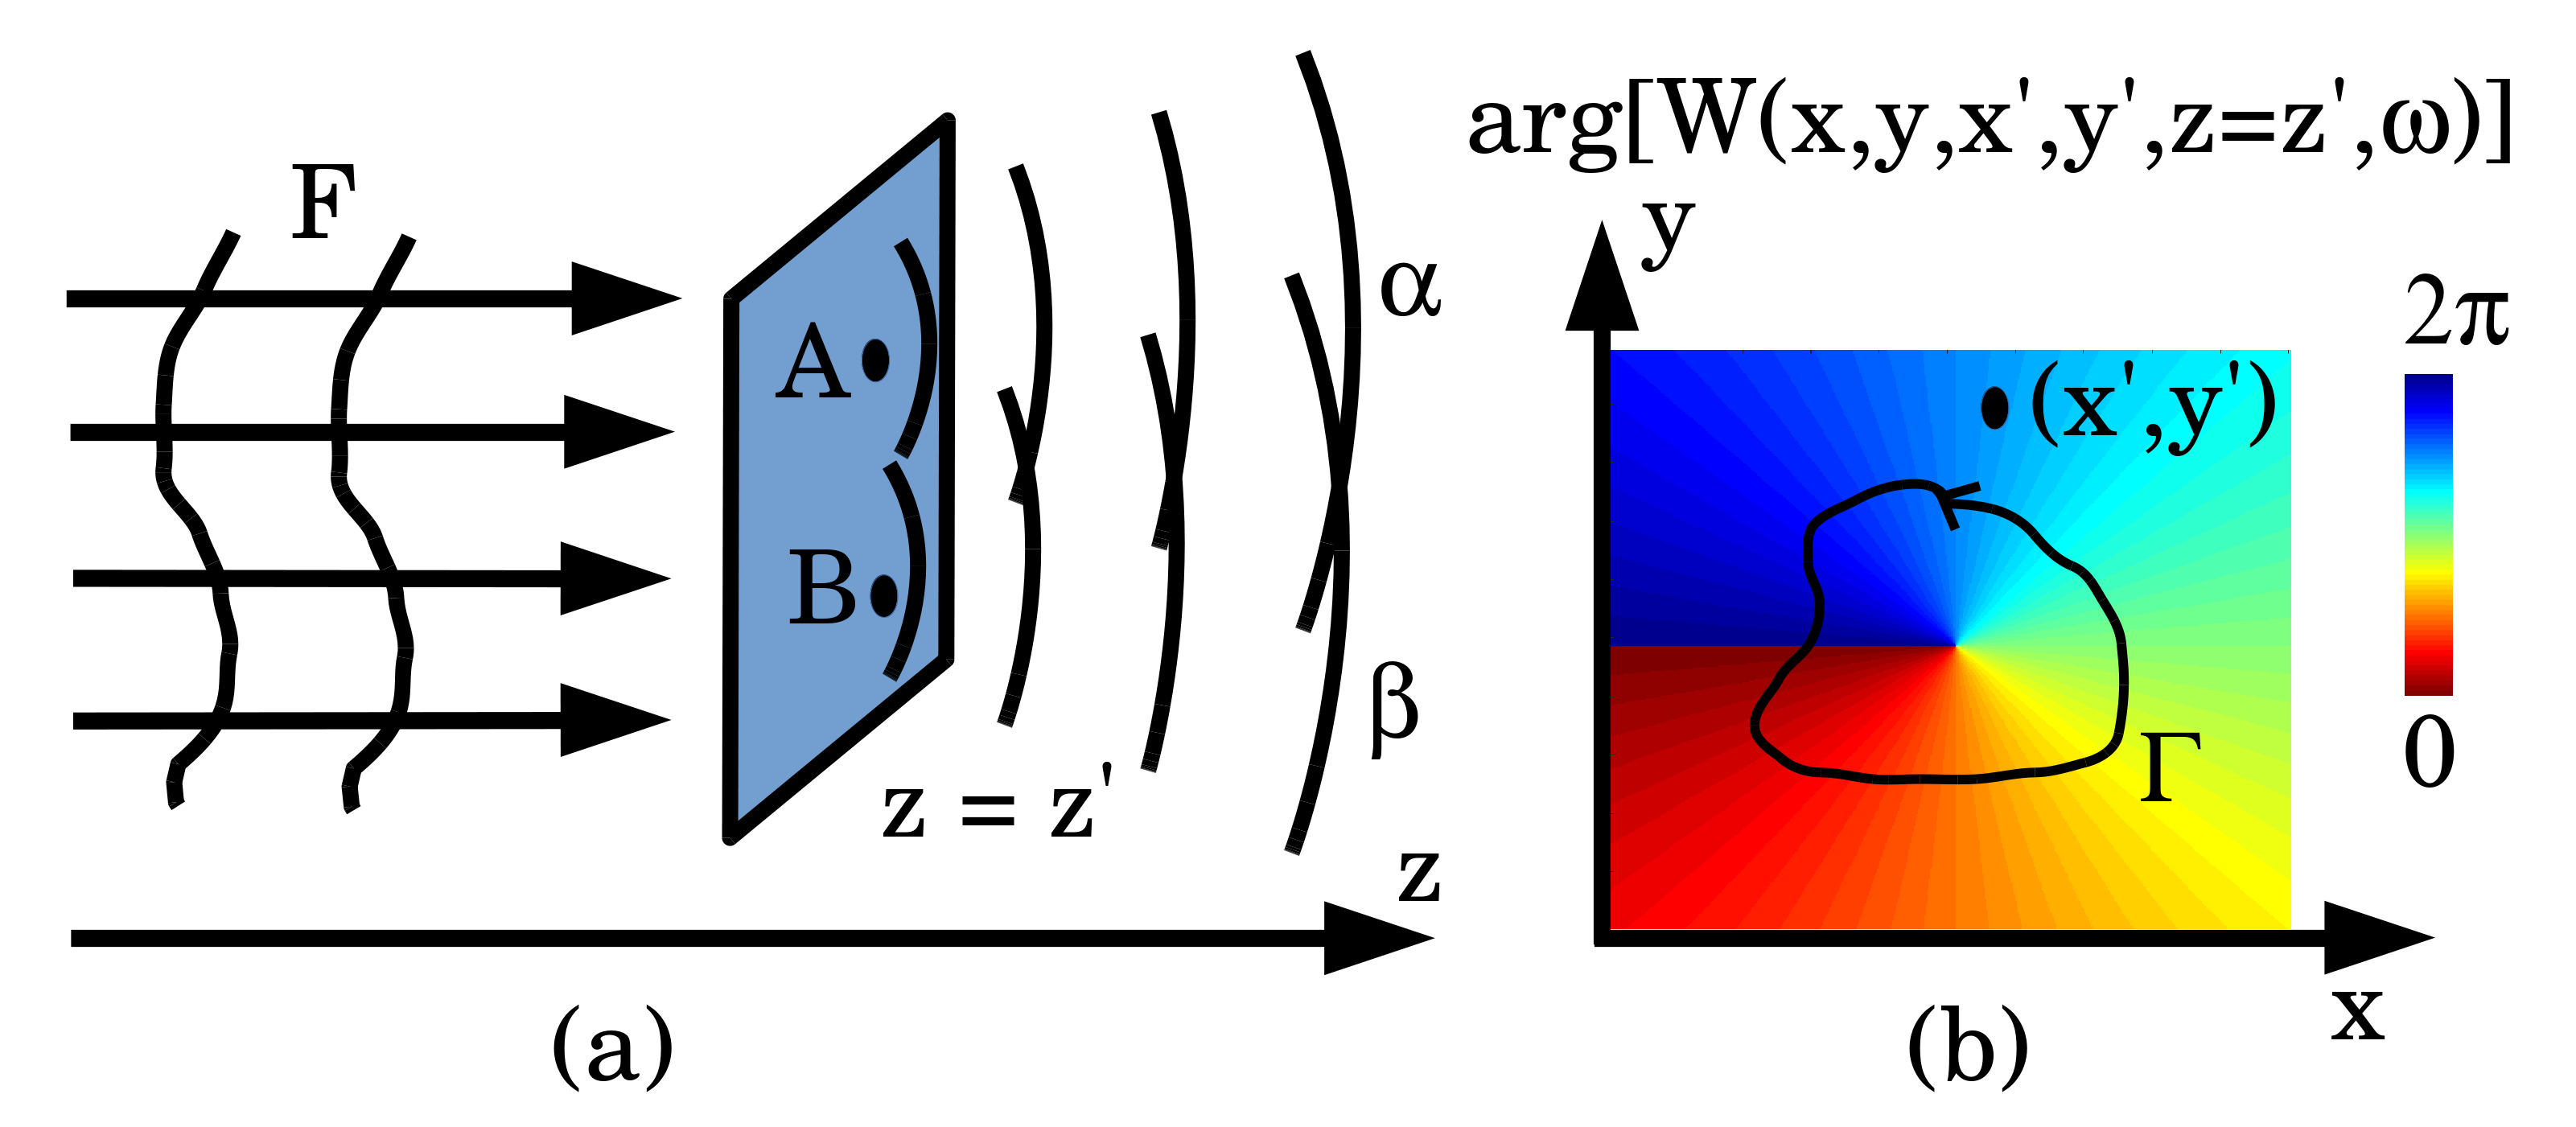
\includegraphics[width=9.0cm]{Figures/coherence_vortex.png}
\label{loss_of_fringe_visibility}
\end{figure}

While $W$ and its magnitude are both single-valued, $\Phi$ will in general be multi-valued. Indeed, since the phase of a complex number is only defined modulo $2\pi$ radians, it may wind by an integer multiple of $2\pi$ in the following manner (see Fig.~\ref{loss_of_fringe_visibility}b) \cite{GburVisser2003}: 
\begin{equation}
\begin{aligned}
\label{phase_of_W_winding}
\oint_{\Gamma} d\Phi(x_1,y_1,x_2,y_2,z,\omega)=2\pi m.
\end{aligned}
\end{equation}
Here, $\Gamma$ is any smooth closed clockwise-traversed one-dimensional curve embedded in the six-dimensional space with coordinates $(x_1,y_1,x_2,y_2,z,\omega)$, $m$ is an integer and $d\Phi$ is the increment in $\Phi$ corresponding to an infinitesimal line segment of $\Gamma$.  Admissible curves $\Gamma$ are those for which $W$ is non-zero at every point on $\Gamma$, ensuring $\Phi$ and hence $d\Phi$ to be well defined at each point on $\Gamma$.  A non-zero $m$ indicates the presence of non-trivial topology in the phase of $W$, with the phase map in Fig.~\ref{loss_of_fringe_visibility}b being one of infinitely many Riemann sheets describing a screw dislocation threaded by the coherence-vortex core. 

When $m$ is non-zero, a coherence vortex \cite{GburVisser2003} is said to be present.  The integer $m$ is the {\em topological charge} of the coherence vortex.  Such structures are a partially-coherent analogue of phase vortices that may form in the phase of coherent optical fields \cite{NyeBerry1974,Nye1999,SoskinVasnetsov2001,DennisProgOpt2009}.  Two key physical consequences of non-vanishing $m$ are outlined below.  These arguments are topological in nature, and restrict consideration to generic structures, namely those that are stable with respect to continuous deformation of the underlying fields. 

The existence of any {\em one} circuit $\Gamma$ for which $m$ is non-zero, implies the presence of a (nodal) manifold of points in $(x_1,y_1,x_2,y_2,z,\omega)$-space, at each of which $W$ vanishes.   Such points are termed correlation singularities, nodal points, nodal lines, or a nodal manifold.  If $\Gamma$ lies in a particular two-dimensional plane $\Pi$ with coordinates $(\xi,\eta)$ within $(x_1,y_1,x_2,y_2,z,\omega)$-space, the so-called coherence vortex \cite{GburVisser2003} will typically occur at a (zero-dimensional) nodal point $(\xi_0,\eta_0)$ in the said plane, serving as a branch point for $\Phi$, about which $\Phi$ winds by $2 \pi m$ radians ({\em cf.} the $m=1$ case in Fig.~\ref{loss_of_fringe_visibility}b).  The set of nodal points becomes a (one-dimensional) nodal line, or a connected set of nodal lines which either form closed loops or extend to the boundary of the considered region, when one considers the one-dimensional loop $\Gamma$ to be embedded within a three-dimensional hyperplane in  $(x_1,y_1,x_2,y_2,z,\omega)$-space.  This set of nodal lines (any point on which is a singular point for $\Phi$) may form a tree-like structure, e.g. if an $m=2$ coherence vortex decays to a pair of $m=1$ coherence vortices \cite{TopologicalReactionsCohVortices,GburSPIE}.  Knotted and braided coherence-vortex nodal lines in $W$ are also topologically possible, albeit exotic.  Permissible nodes in tree-like nodal-line structures in $W$ are governed by the law of conservation of topological charge.  This set of nodal lines becomes a two-dimensional network of nodal sheets (zero sheets) in any four-dimensional hyperplane within the $(x_1,y_1,x_2,y_2,z,\omega)$-space, and a three-dimensional manifold of nodal points in any five-dimensional hyperplane subset of $(x_1,y_1,x_2,y_2,z,\omega)$-space.  Finally, in the full six-dimensional $(x_1,y_1,x_2,y_2,z,\omega)$-space, the set of nodal points of $W$ will form a four-dimensional network of points $C$, at each of which $W$ vanishes \cite{Marasinghe2010}.  

These nodal points in $W$ exhibit ``complete destructive interference of coherence''.  Stated more precisely, any point $(x_1',y_1',x_2',y_2',z',\omega)$ in the correlation-singularity manifold $C$ will correspond to a pair of spatial points $(x_1',y_1',z')\equiv A$ and $(x_2',y_2',z')\equiv B$ for which the partially-coherent disturbance is completely uncorrelated at angular frequency $\omega$ \cite{Schouten2003,GburVisser2003,Bogatyryova2003}.  If, for example, a point scatterer were to be placed at $A$, with another point scatterer at $B$, and the radiation scattered from both points allowed to overlap, no interference fringes would be observed if the resulting diffracted fields were to be filtered to angular frequency $\omega'$.  See Fig.~\ref{loss_of_fringe_visibility}b, together with the grey curve (curve 1) in Fig.~\ref{Young_fringe_anholonomy}.  The manifold of points $C$, which will typically permeate much of the $(x_1,y_1,x_2,y_2,z,\omega)$-space associated with cross-spectral densities calculated for non-trivial systems \cite{TopologicalReactionsCohVortices,GburVisser2003}, is akin to a web of incoherence that permeates a partially-coherent field's cross-spectral density.

\begin{figure}
\caption{Ratcheting of Young-type interferograms associated with an $m=1$ coherence vortex.  (a) A series of Young-type interferometers is constructed.  In all of these setups, radiation illuminates a screen in which the first of two pinholes is always at $B$.  The second pinhole is placed at $A$, before being moved through the cycle of locations $C1 \rightarrow C2 \rightarrow C3 \rightarrow C4 \rightarrow C1$.  (b) The resulting Young-type intereferograms, over some plane downstream of the points scatterers, are shown in curves 1 (pinholes $A$ and $B$), 2 ($C1$ and $B$), 3 ($C2$ and $B$), 4 ($C3$ and $B$), 5 ($C4$ and $B$) and 6 ($C1$ and $B$) respectively. Note that curves 2 and 6 are identical.  Also, $I(x)$ denotes the spectral density of the interferogram as a function of the transverse coordinate $x$, perpendicular to the optic axis.}
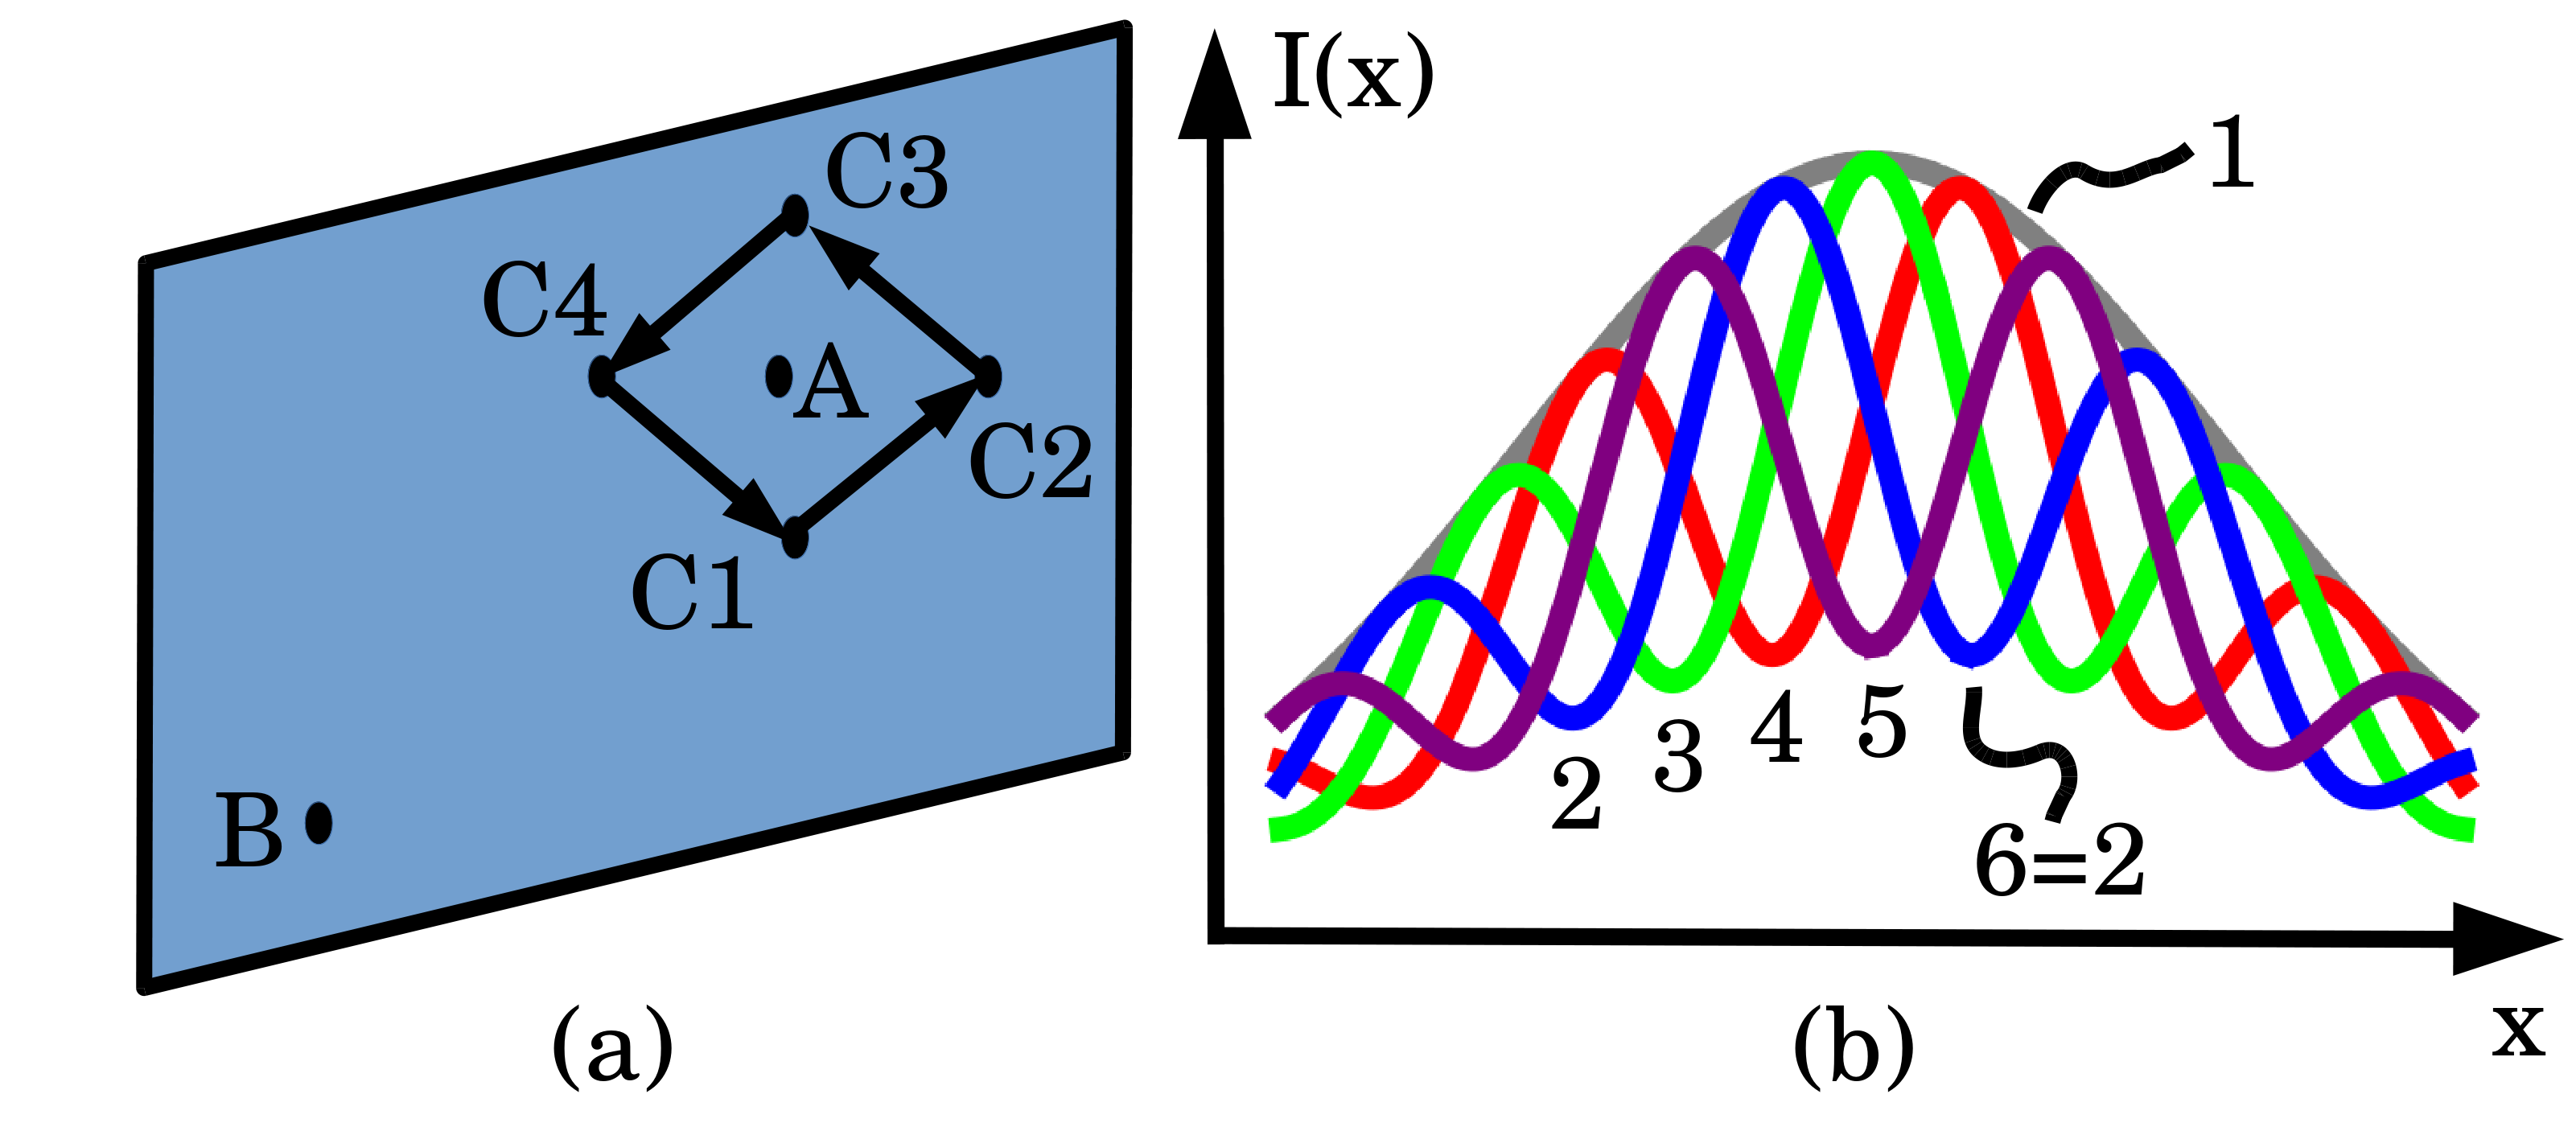
\includegraphics[width=9.0cm]{Figures/Anholonomy.png}
\label{Young_fringe_anholonomy}
\end{figure}

A second key consequence, of the coherence-vortex web permeating the cross-spectral density, is again related to the visibility of interference fringes associated with pairs of scattering points.  As previously stated, when pinholes are placed at locations $A$ and $B$ in Fig.~\ref{loss_of_fringe_visibility} that correspond to a coherence vortex (see also Fig.~\ref{Young_fringe_anholonomy}(a)), there is zero fringe visibility in the associated Young-type pattern filtered to energy $\hbar \omega$: see curve 1 in Fig.~\ref{Young_fringe_anholonomy}(b).  However, the non-zero fringe visibility is regained if one moves ``off the coherence vortex'' by shifting the first pinhole from location $A$ to location $C1$: see curve 2 in Fig.~\ref{Young_fringe_anholonomy}(b).  The vortical nature of the coherence vortex is then manifested if one performs a sequence of Young-type interference experiments, where the pinhole at $B$ is kept fixed, while the pinhole at $C1$ is moved through the cycle of locations $C1$ (curve 2), $C2$ (curve 3), $C3$ (curve 4), $C4$ (curve 5) and finally back to $C1$ (curve 6 = curve 2). If one traces the evolution of the intensity maxima associated with the sequence of Young-type interferograms in curves 2 to 6, the physical meaning of $m$ becomes clear: during the cycle, if $m=1$ then the maxima of the interferogram will ``ratchet'' to the right by one fringe during the cycle. If $m=-1$ they would instead ratchet to the left by one fringe during the cycle.  For general $m$, the fringes would ratchet to the right (left) by $|m|$ fringes, if $m$ is positive (negative) \cite{Marasinghe2010}.

\section{Simulations}

The coherent mode decomposition of undulator radiation emitted by a 1.4 meter long U18 undulator (period of 18.3 mm), which is to be placed at the centre of straight section of the EBS (6 GeV, 147 pm$\times$rad emittance storage ring), is here performed using COMSYL. The undulator is tunned at 17.226 keV (K=0.411) and the flux there is 2.8 $\times 10^{14}$ photons/s/0.1\%bw in 1$\times$1 mm$^2$ apertute at 30 m. Figure~\ref{cumulative_mode_occupation} shows the cumulative occupation of the modes, defined as: 
\begin{equation}
\begin{aligned}
\label{spectrum}
d_n=\frac{\sum_{m=0}^{n} \lambda_m}{\sum_{m=0}^{\infty} \lambda_m}.
\end{aligned}
\end{equation}

From this plot it can be seen that the 1100 coherent modes calculated contain almost all (98\%) of the emitted radiation. The coherence fraction (occupation of the first mode) is 2.8\%. The cumulation of the first 10 modes contain 21.7\% of the emitted intensity and 33.0\% (20 modes), 73.3\% (100 modes) and 97.9\% (1000 modes). 
Figure~\ref{spectral_density} shows the spectral spatial extension of the spectral density (intensity) at the source plane, and also the extension of the first mode.
Indeed, as shown in Fig.~\ref{spectral_density} it is necessary to account for a few hundred modes to represent more than 90\% of the spectral density. The spectral density FWHM (Full Width at Half Maximum) dimensions are 71.3$\times$10.9 $\mu$m$^2$. These values are in good agreement with simple estimations considering the source size as a convolution of the undulator emission $\sigma_\gamma\approx (2.74/4\pi) \sqrt{\lambda L}\approx$9.6 $\mu$m ($\lambda$ is the radiation wavelength and L is the undulator length) with the size of the electron size ($\sigma_x$=30.2$\mu$m, and $\sigma_y$=1.37$\mu$m for the EBS straight section) that give FWHM values of 71.3$\times$10.0 $\mu$m$^2$. The size (FWHM) of the first mode is 12.4$\times$6.11 $\mu$m$^2$.  

\begin{figure}\label{cumulative_mode_occupation}
\caption{Cumulative mode occupation for the emission of an undulator U18 placed at the EBS lattice and tuned to a photon energy of 17.226 keV.}
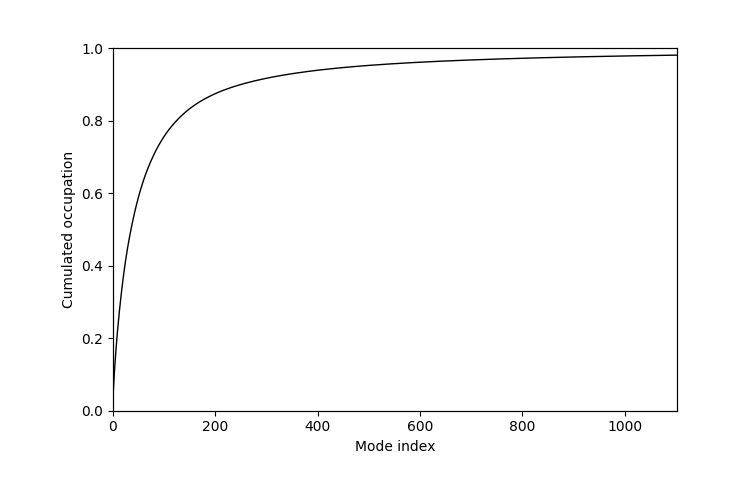
\includegraphics[width=9.0cm]{Figures/vx_cumulated.png}
\end{figure}

\begin{figure}\label{spectral_density}
\caption{Top: Spectral density (intensity) distribution at the source plane. Bottom: Intensity of the first coherent mode at the source plane.}
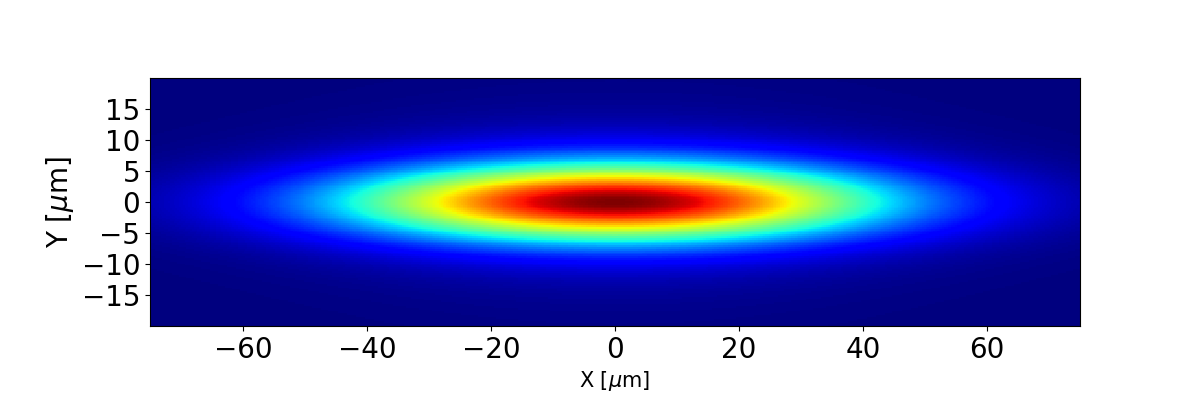
\includegraphics[width=9.0cm]{Figures/spectral_density_upto1099.png}
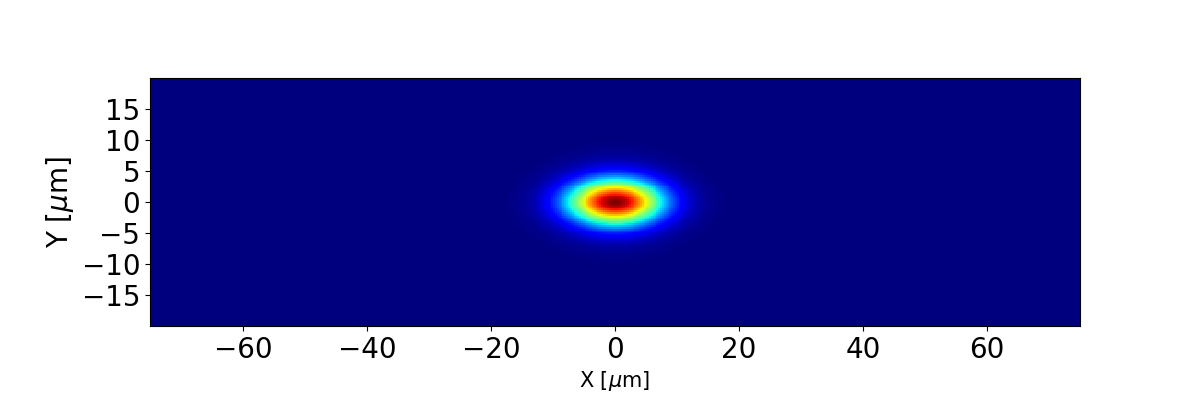
\includegraphics[width=9.0cm]{Figures/spectral_density_upto0.png}
\end{figure}

Before proceeding further, we note from Figure~\ref{spectral_density} that the first coherent mode is non-zero (or, more precisely, non-negligible) over an area which is smaller than the area over which the spectral density is non-zero (non-negligible). Such a property will typically be true for a large class of partially-coherent beams, which will necessarily have at least two coherent modes since they are not fully coherent, by assumption.  This typical property follows directly from the fact that the spectral density of the beam is given by the sum of the spectral densities of each of the coherent modes, hence the area over which the spectral density is non-zero is always non-contracting as one adds progressively more coherent modes, irrespective of the particular non-zero eigenvalues associated with the said modes.  

Now, for the example shown in Figure~\ref{spectral_density}, the region over which the total spectral density is greater than some threshold value (say, 1\% of the maximum value) is roughly elliptical.  Let us denote this essential support of the spectral density by $\mathcal{S}$.  If the cross-spectral density were to vanish for any pair of points $(r_1,r_2)$, with $r_1 \in \mathcal{S}$ and $r_2 \in \mathcal{S}$, then then this must be associated with a zero of the mutual coherence function $\mu$ (normalised cross-spectral density).  The proof of this fact \cite{GburSPIE} is as follows.  Recall that the cross-spectral density $W$, spectral density $S$ and mutual coherence function (normalized CSD) $\mu$ are related by $W(r_1,r_2,\omega)=\sqrt{S(r_1,\omega)}\sqrt{S(r_2,\omega)}\mu(r_1,r_2,\omega)$.  Since, by construction, $S(r_1,\omega)$ cannot vanish when $r_1 \in \mathcal{S}$, and $S(r_2,\omega)$ cannot vanish when $r_2 \in \mathcal{S}$, the null factor law implies that $W(r_1\in \mathcal{S},r_2\in \mathcal{S},\omega)$ can vanish if and only if $\mu(r_1\in \mathcal{S},r_2\in \mathcal{S},\omega)$ vanishes.  If there is one dominant coherent mode, it will typically be difficult to attain such zeros of the mutual coherence function, when both $r_1$ and $r_2$ lie within the region where the intensity of the first coherent mode is large.  However, this restriction vanishes when either or both of $r_1$ and $r_2$ lies outside the essential support of the dominant coherent mode.  While we put this observation to one side for the moment, we note that it guides the simulations given later in the present section.        

\begin{figure}
\caption{Schematic representation of the different positions (A,B,C) for the point $\vec{r_2}$ (see text). The largest oval represents the spectral density (Fig.~\ref{spectral_density}a), and the inner circle the region over which the squared modulus of the first mode is non-negligible (Fig.~\ref{spectral_density}b).
The points coordinates (in $\mu$m) are: A=(0,0), B=(9.52,4.76) and C=(20.83,9.82)}
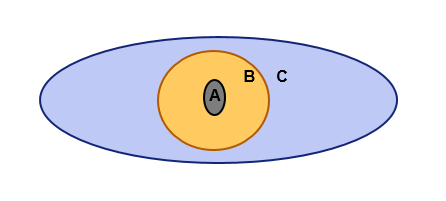
\includegraphics[width=7.5cm]{Figures/eye.png}
\label{eye}
\end{figure}

Returning to the numerical simulation, our next task is to extract the CSD phase. Being a 4D function, it is convenient to fix two variables ({\em e.g.} components of the position $\vec{r_2}$) and observe how the phase depends on the other two transverse spatial coordinates. Hence, several points have been chosen (Fig.~\ref{eye}) The first position (point A) is at the centre of the emission. The second (point B) is at a non-centred position where the first mode has appreciable intensity. The third one (point E) is outside the first mode, but in a place with appreciable intensity. Indeed, the core of a coherence vortex always exactly coincides with pair of spatial positions having zero CSD. It is however useless to discuss the phase variations in position with zero (or close to zero) magnitude of the CSD. Therefore, in our representation of the phase in false colours (Fig.~\ref{pointP}) the transparency of the pixel is related to the intensity, in such a way that the pixels with zero intensity appear as white. 

When $\vec{r_2}$ is set to position $A$, we have the plot of the phase $\Phi(x,y,x_A,y_A)$ of the CSD, as shown in Fig.~\ref{pointP}A, as a function of the coordinates $(x,y)$ of $\vec{r_2}$, with $z_1, z_2$ and $\hbar\omega$ all having the previously-indicated fixed values.  As previously mentioned, the brightness of the displayed phase has been taken to be proportional to $|W(x,y,x_A,y_A)|$, since CSD phase is not meaningful when $|W(x,y,x_A,y_A)|$ is negligible.  The figure shows four maps for the CSD phase, corresponding to the number $n$ of non-dominant coherent modes being 1, 10, 100, and 1000 (from top to bottom).  When only one coherent mode is included, there are no topological defects in the CSD phase.  However, when 10 non-dominant coherent modes are included, as in panel (b), non-vortical domain-wall defects in the CSD appear: three such structures are marked.  Across each of these CSI-phase domain walls, the phase $\Phi$ of the CSD jumps by $\pi$ radians, with the CSD itself vanishing along each of the lines through which $\Phi$ changes discontinuously.  Note that such CSI-phase domain walls were the first CSD singularities to be reported, in a classic study by Schouten {\em et al.} \citeyear{Schouten2003}.  Adding more coherent modes, to the case of $n=100$, the domain walls become curved and the domain over which the CSD is non-negligible widens.  Finally, for the case  $n=1000$, the effect of the increasing number of coherent modes is to narrow the region over which the CSD is non-negligible.  The general trend from top panel through the bottom one is therefore a reduction in the spatial extent over which two-point field correlations have a magnitude $|W(x,y,x_A,y_A)|$ that is non-negligible, when one of the points is taken to be point $A=(x_A,y_A)$ at the centre of the beam.           

When $\vec{r_2}$ is set to position $B$, we have the plot of the phase $\Phi(x,y,x_B,y_B)$ of the CSD, as shown in Fig.~\ref{pointP}B, as a function of the coordinates $(x,y)$ of $\vec{r_2}$.  This figure again shows four maps for the CSD phase, corresponding to the number $n$ of non-dominant coherent modes being 1, 10, 100, and 1000.  A similar trend to the previous figure is observed with regard to domain walls.  The additional feature of coherence vortices becomes manifest.  Indeed, as one adds more coherent modes, to the case of $n=1$ which is shown in panel (a), the topologically-unstable domain walls begin to dissolve into the topologically stable CSD-phase defects, namely the coherence vortices that form the key topic of the present paper. These coherence-vortex cores are evident as points upon which all phase-value colours converge like spokes on a wheel, with an associated vanishing of the modulus of $W(x,y,x_B,y_B)$ and an increasing speckled structure to the CSD.  \todo{Several such coherence-vortex cores have been labelled with arrows, in panels (b) and (c)}.  One feature evident in the associated CSD is the speckled structure in panel including 100 coherent modes, with the CSD being localised to speckled ``islands'' where the CSD is non-negligible, with each such ``island'' having a different and essentially random phase when compared to its neighbours.  Such a ``patchy'' structure, which is also observed {\em e.g.} in the Wigner function associated with chaotic quantum systems \cite{Zurek}, will evidently influence quantities that are derived from the cross-spectral density via suitable coarse-graining.

\begin{figure}
\caption{Phase as a function of $(x,y)$ of $W(x,y,x_P,y_P)$, with P=A,B,C (see text), when the number $n$ of non-dominant coherent modes is (from top to bottom) 1, 10, 100, and 1000. The brightness of the displayed phase is proportional to $|W(x,y,x_P,y_P)|$, since CSD phase is not meaningful when $|W(x,y,x_P,y_P)|$ is negligible. In each image, a circle marks the position of the point P.}
A~~~~~~~~~~~~~~~~~~~~~~~~~~~~B~~~~~~~~~~~~~~~~~~~~~~~~~~~~C\\
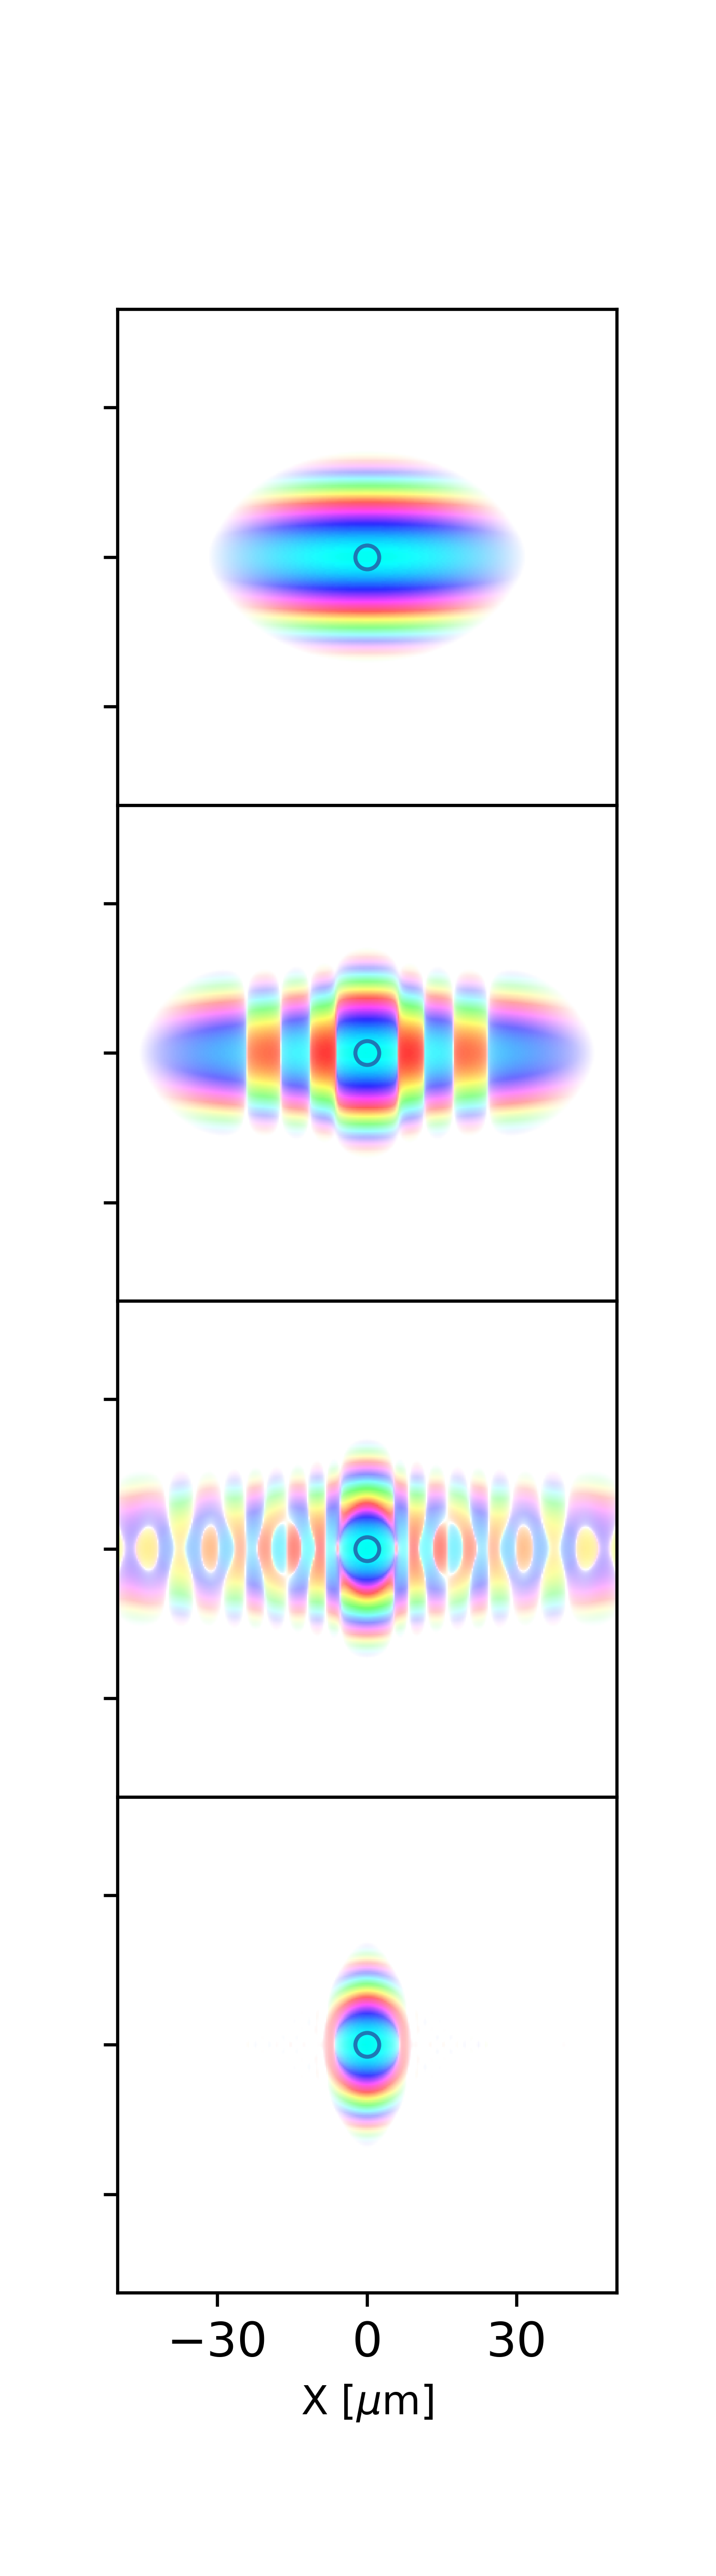
\includegraphics[width=2.75cm]{Figures/vx_id16a_A.png}
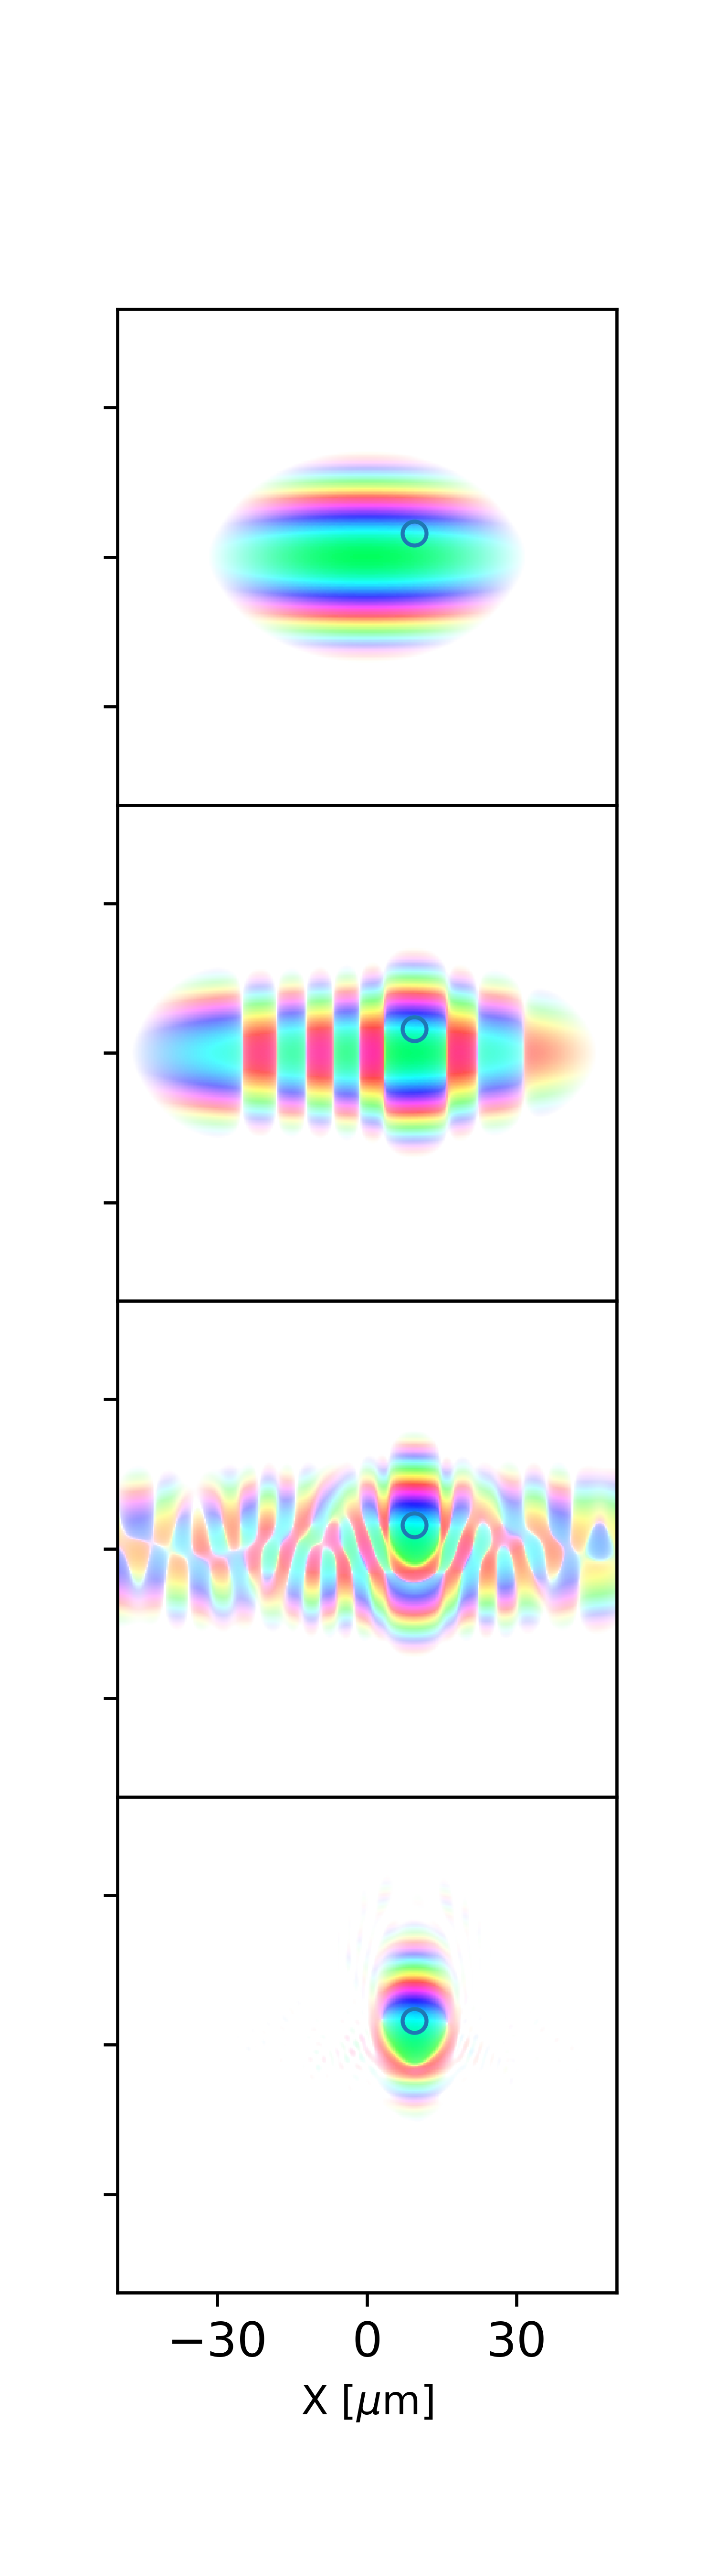
\includegraphics[width=2.75cm]{Figures/vx_id16a_B.png}
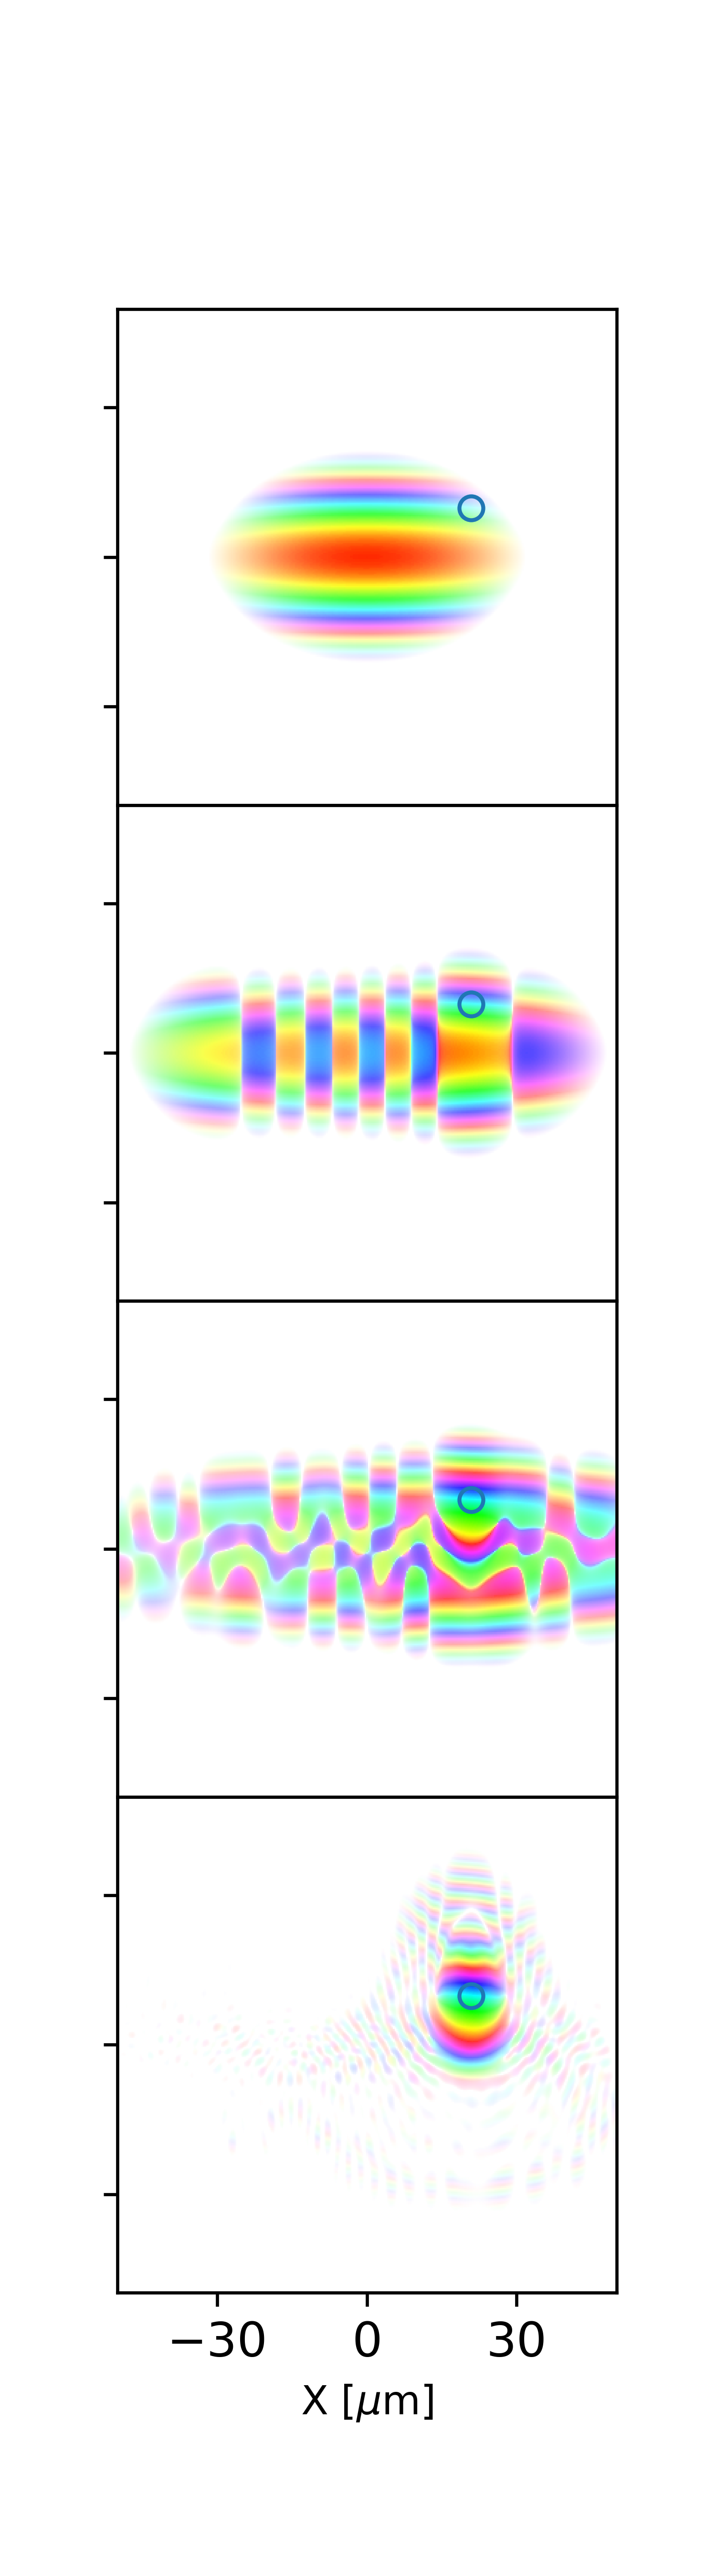
\includegraphics[width=2.75cm]{Figures/vx_id16a_C.png}
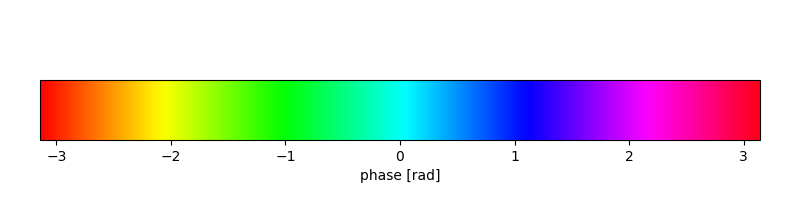
\includegraphics[width=7cm]{Figures/color_bar.png}
\label{pointP}
\end{figure}

As a third and final example, when $\vec{r_2}$ is set to position $C$, we have the plot of the phase $\Phi(x,y,x_C,y_C)$ of the CSD, as shown in Fig.~\ref{pointP}C.  Unlike the previous two examples, now the fixed spatial coordinate $C$ lies outside the dominant first mode's intensity distribution, but within the region where the spectral density of the entire beam is non-negligible.  We again see the previously-described trends, but with the (generic, stable) coherence vortices being rather more prevalent than the (non-generic, unstable) CSD-phase domain walls.    


\section{Simulations of propagated beams}

The calculation of the coherent mode decomposition for the undulator radiation is performed in the source plane, placed the middle of the undulator. It is more realistic to propagate the radiation to a some distance downstream from the source, to a position in which a potential two-slit Young experiment would be feasible. As mentioned before, the propagated CSD is calculated by adding the propagated-modes. Propagation is made using a Fourier Optics Fresnel propagator, including a zoom factor \todo{cite Schmidt and Pirro} that permits to adapt the window for different propagated distances. The propagated first mode and spectral density at a distance D=30 m is shown in Fig.~\ref{spectral_density_propagated}. The FWHM of the spectral density is 431$\times$316 $\mu$m$^2$. Again, for a sanity check, this size can be compared with the propagation (30 m) of the beam divergence estimated as the convolution of the undulator emission divergence $\sigma'_\gamma=0.68\sqrt{\lambda/L}$ with the electron divergences ($\sigma'_x$=3.64 $\mu$rad and $\sigma'_y$=1.37 $\mu$ rad giving 498$\times$366 $\mu$m$^2$ FWHM.). 

\begin{figure}\label{spectral_density_propagated}
\caption{Top: Spectral density (intensity) distribution at a plane placed at 30 m from the source. Bottom: Intensity of the first coherent mode at this plane.}
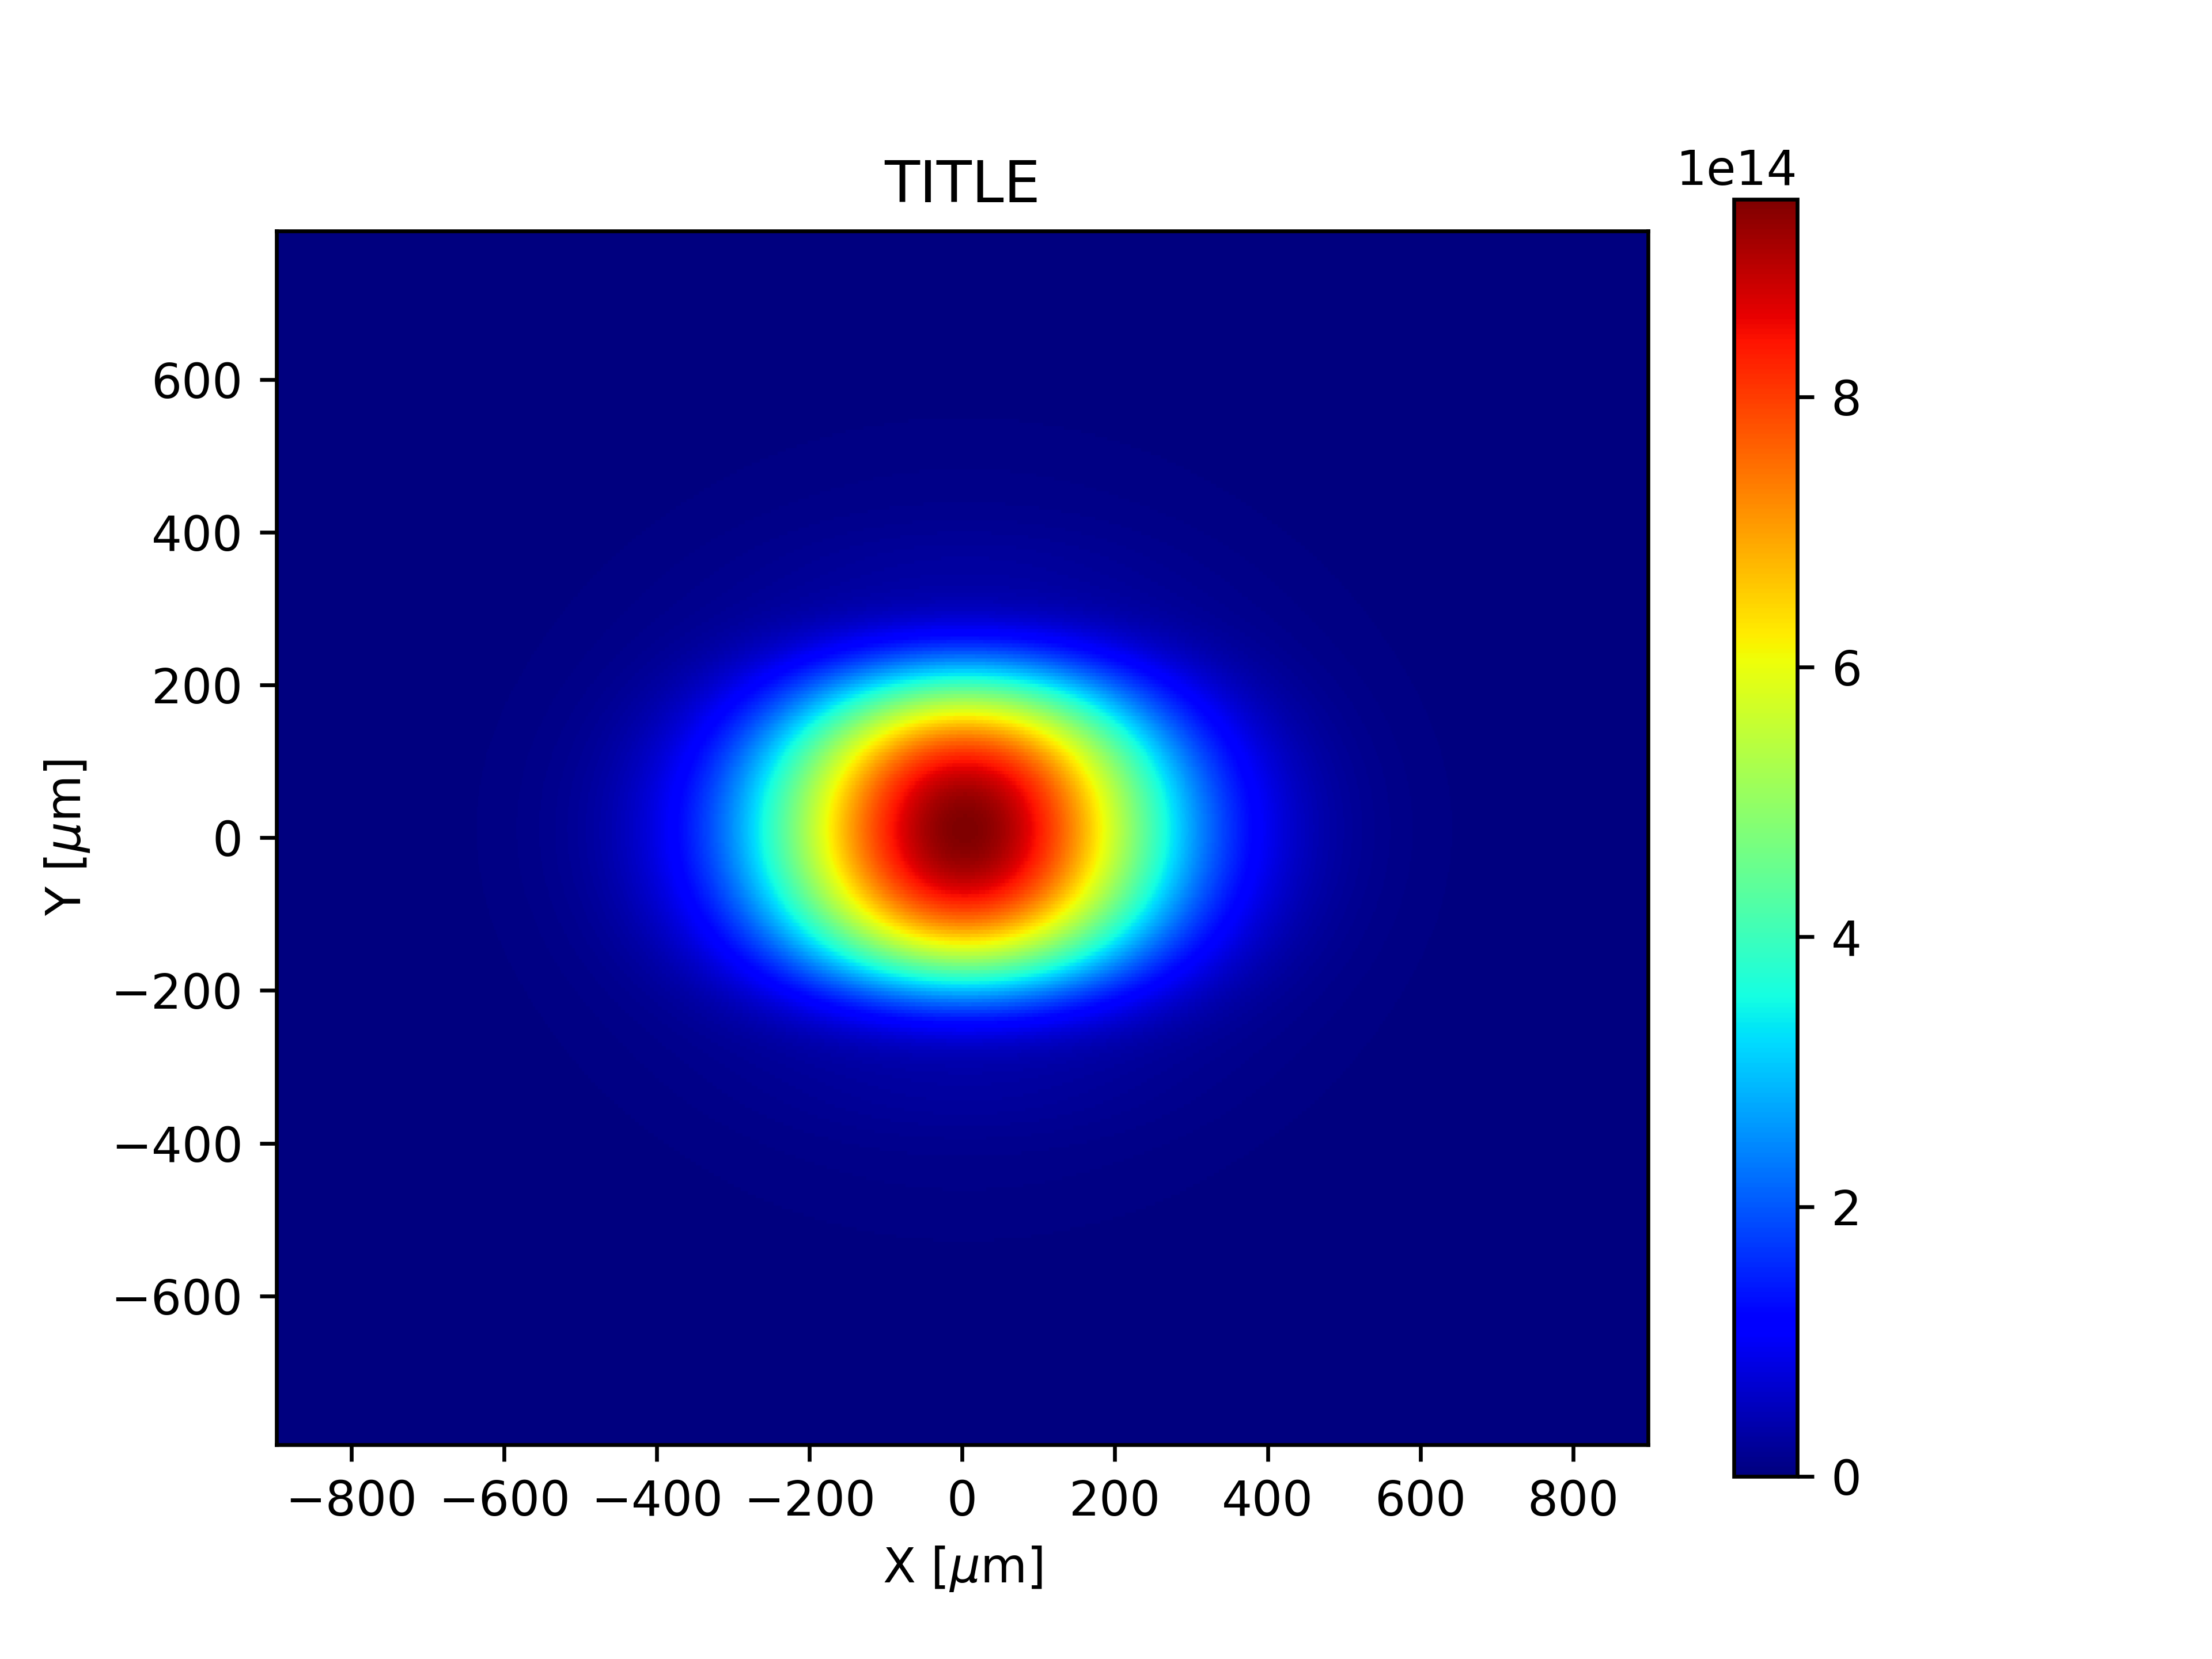
\includegraphics[width=9.0cm]{Figures/spectral_density_upto1099_propagated.png}
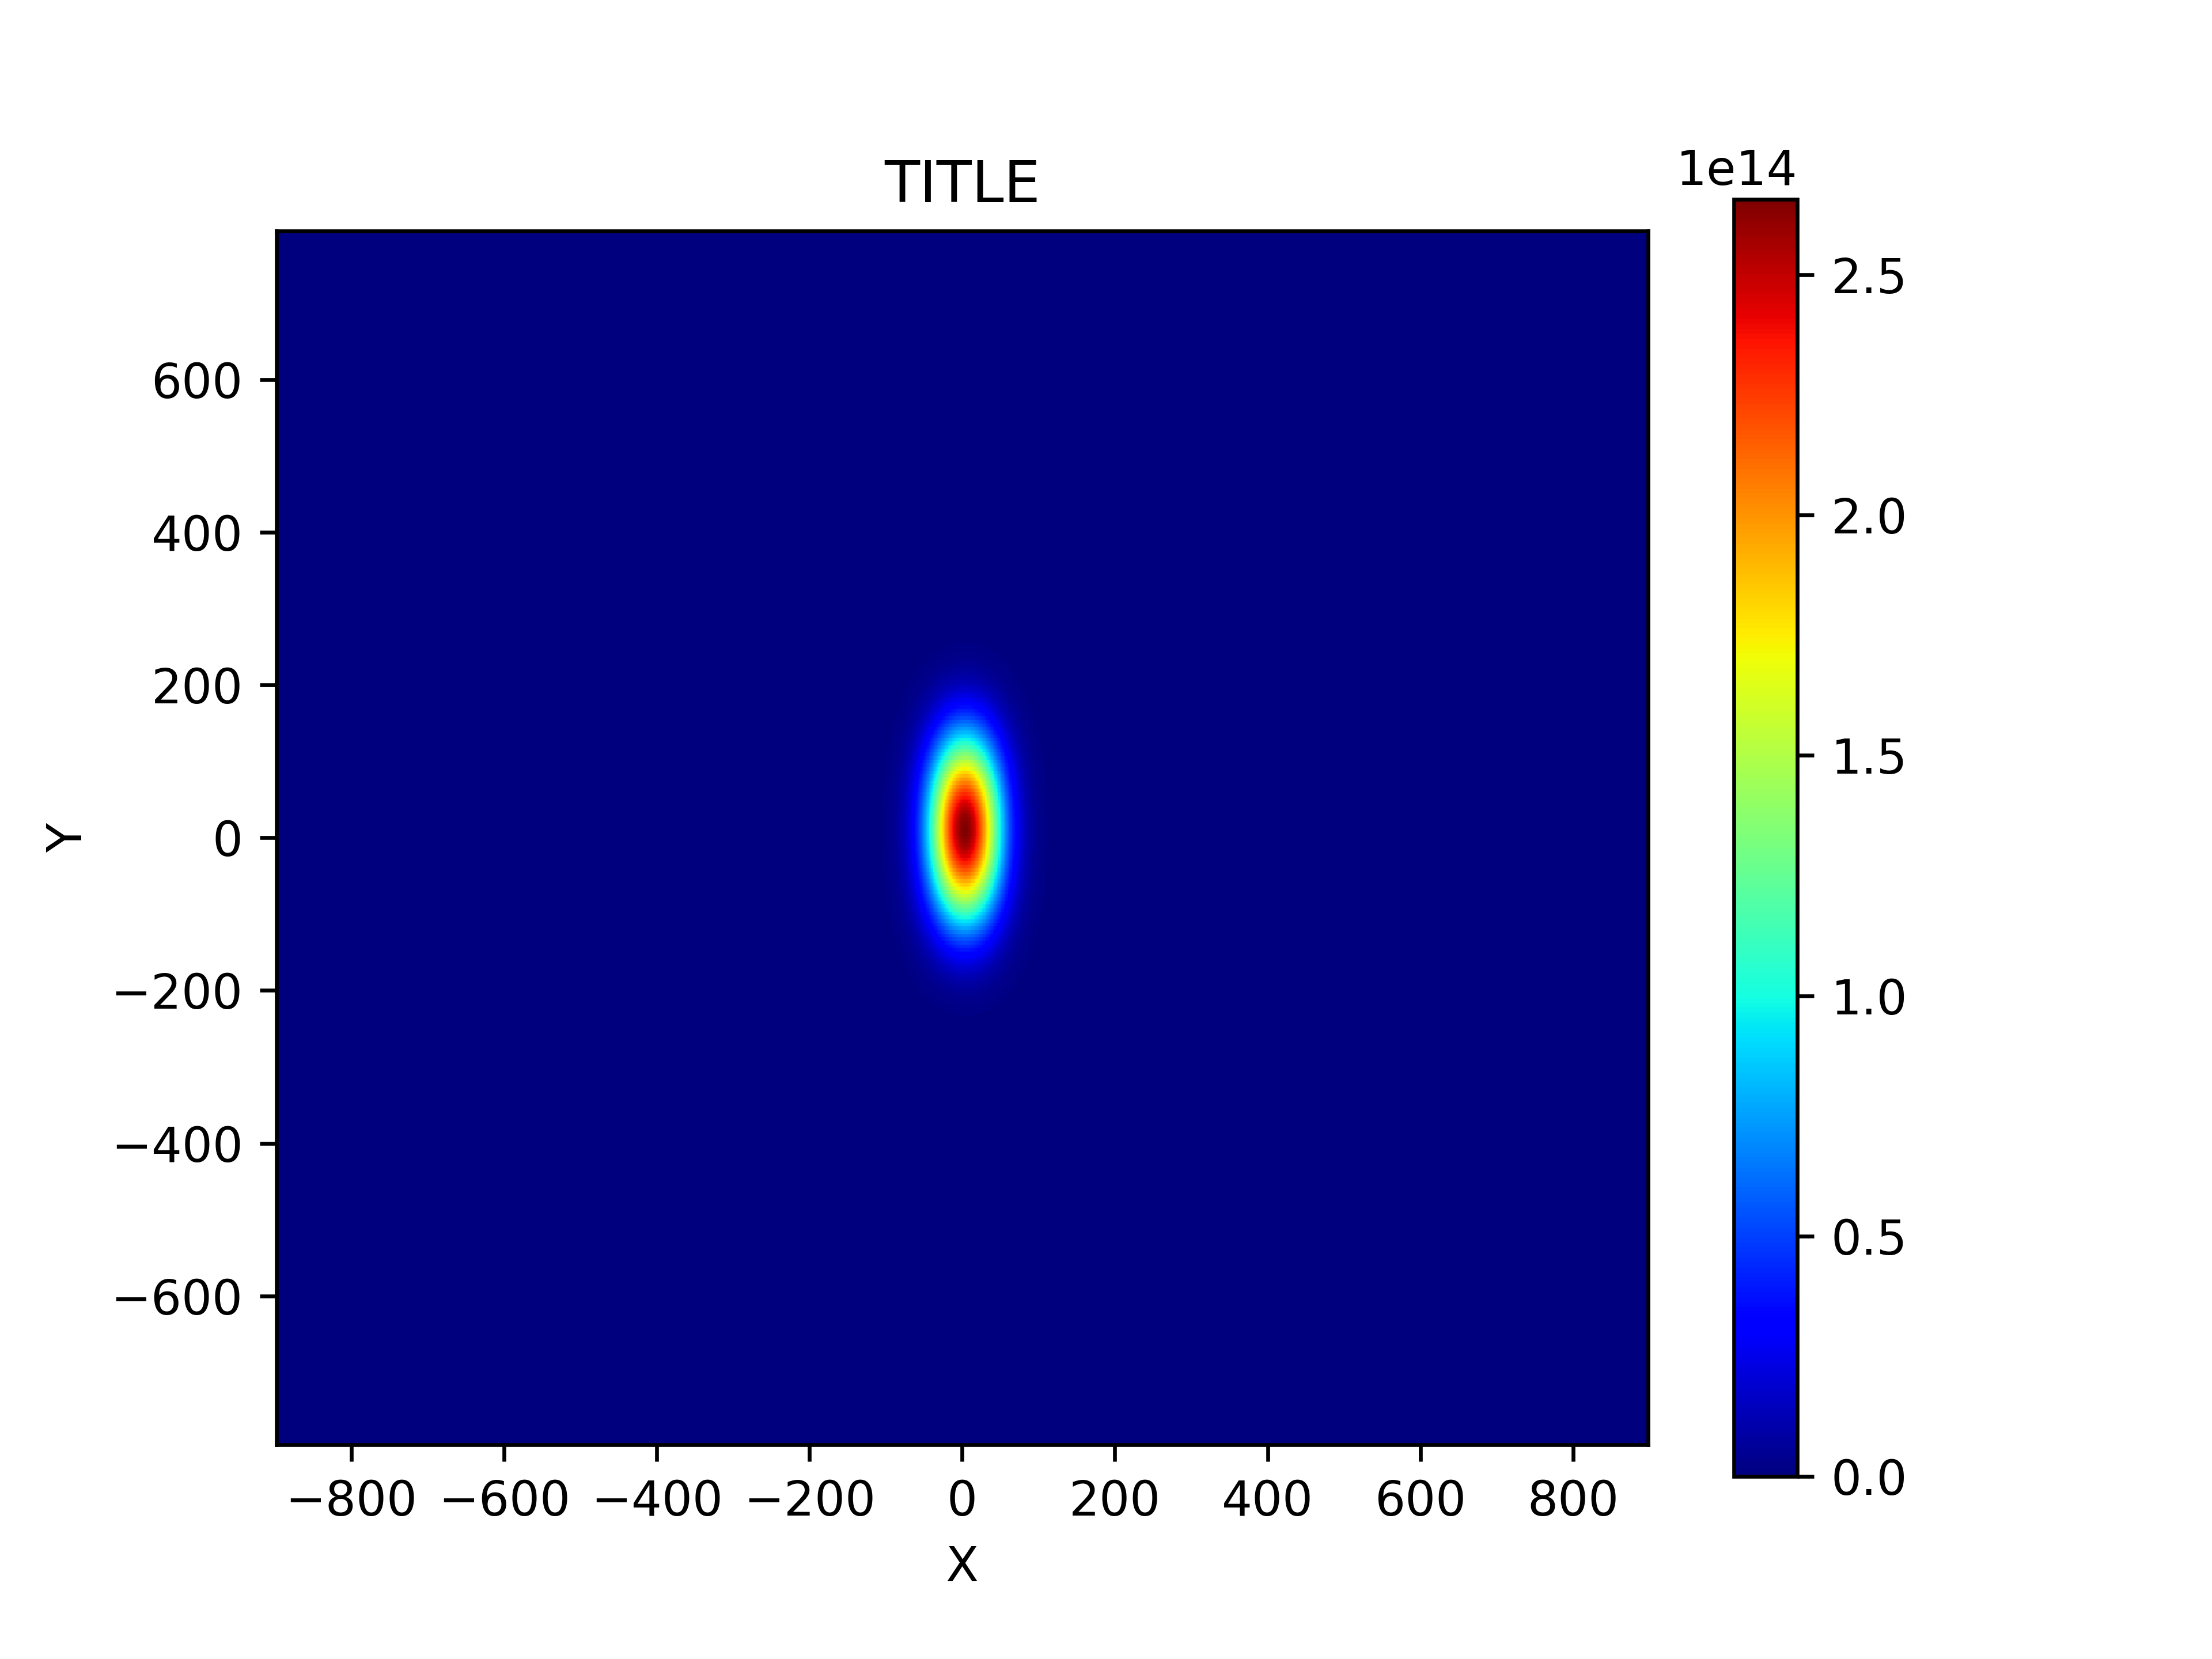
\includegraphics[width=9.0cm]{Figures/spectral_density_upto0000_propagated.png}
\end{figure}

The CSD propagated at ESRF for different fixed points A', B' and C' are shown in Fig.~\ref{points_propagated30}. The coordinates of A',B' and C' have been selected to be homethetic with respect to the position of A,B,C supposing that the FWHM at the source will transform in the FWHM' at the propagated distance. In practice $(x_A/FHWM_{x,D=0},y_A/FHWM_{y,D=0})=x_A'/FHWM_{x,D=30},y_A'/FHWM_{y,D=30})$, and similarly for B and C. This figure shows a very strong variation of the phase. It looks like a sort of far-field regime is attained. In the Fraunhofer regime, the shape of the intensity distribution is not changed, it only expands with distance. A similar behaviour may be expected with the phase. Also, the rich structure of the phase map makes technically difficult to look to the details and identify the exact position and neighbourhood of the vortices. It is therefore more interesting to look to closer propagation distances, in the near field. 


\begin{figure}
\caption{Phase as a function of $(x,y)$ of $W(x,y,x_P,y_P)$ at z=30m, with P=A',B',C', when the number $n$ of non-dominant coherent modes is (from top to bottom) 1, 10, 100, and 1000. The brightness of the displayed phase is proportional to $|W(x,y,x_P,y_P)|$, since CSD phase is not meaningful when $|W(x,y,x_P,y_P)|$ is negligible. \todo{May be remove this plot? I think Fig.~\ref{pointC_propagated} would be sufficient. Perhaps replace 100m propagation there by 30m propagation here?} }
A'~~~~~~~~~~~~~~~~~~~~~~~~~~~~B'~~~~~~~~~~~~~~~~~~~~~~~~~~~~C'\\
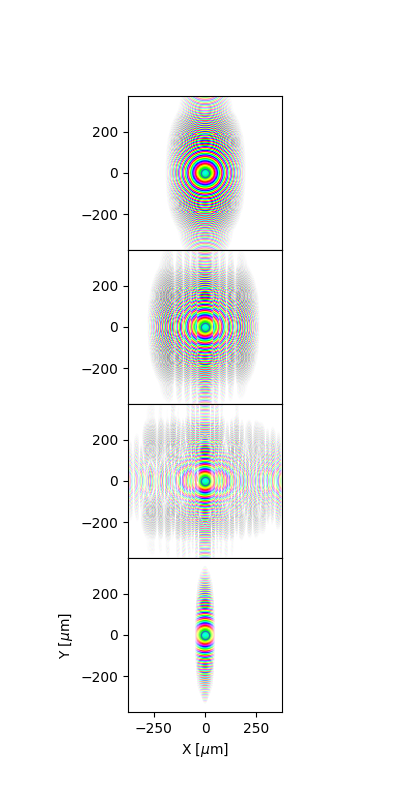
\includegraphics[width=2.75cm]{Figures/vx_id16a_A_propagated.png}
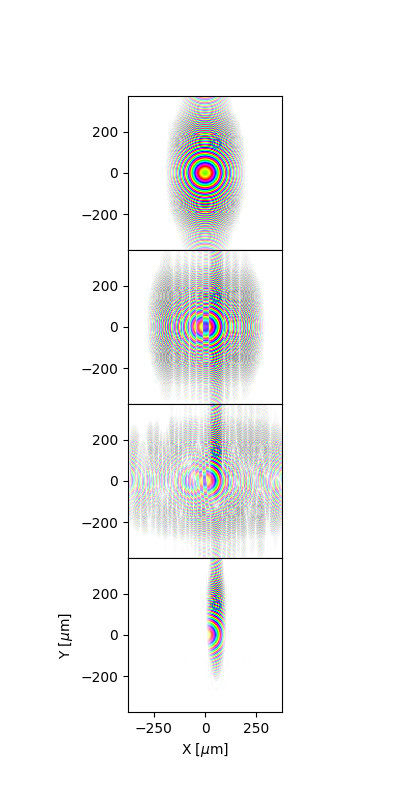
\includegraphics[width=2.75cm]{Figures/vx_id16a_B_propagated.png}
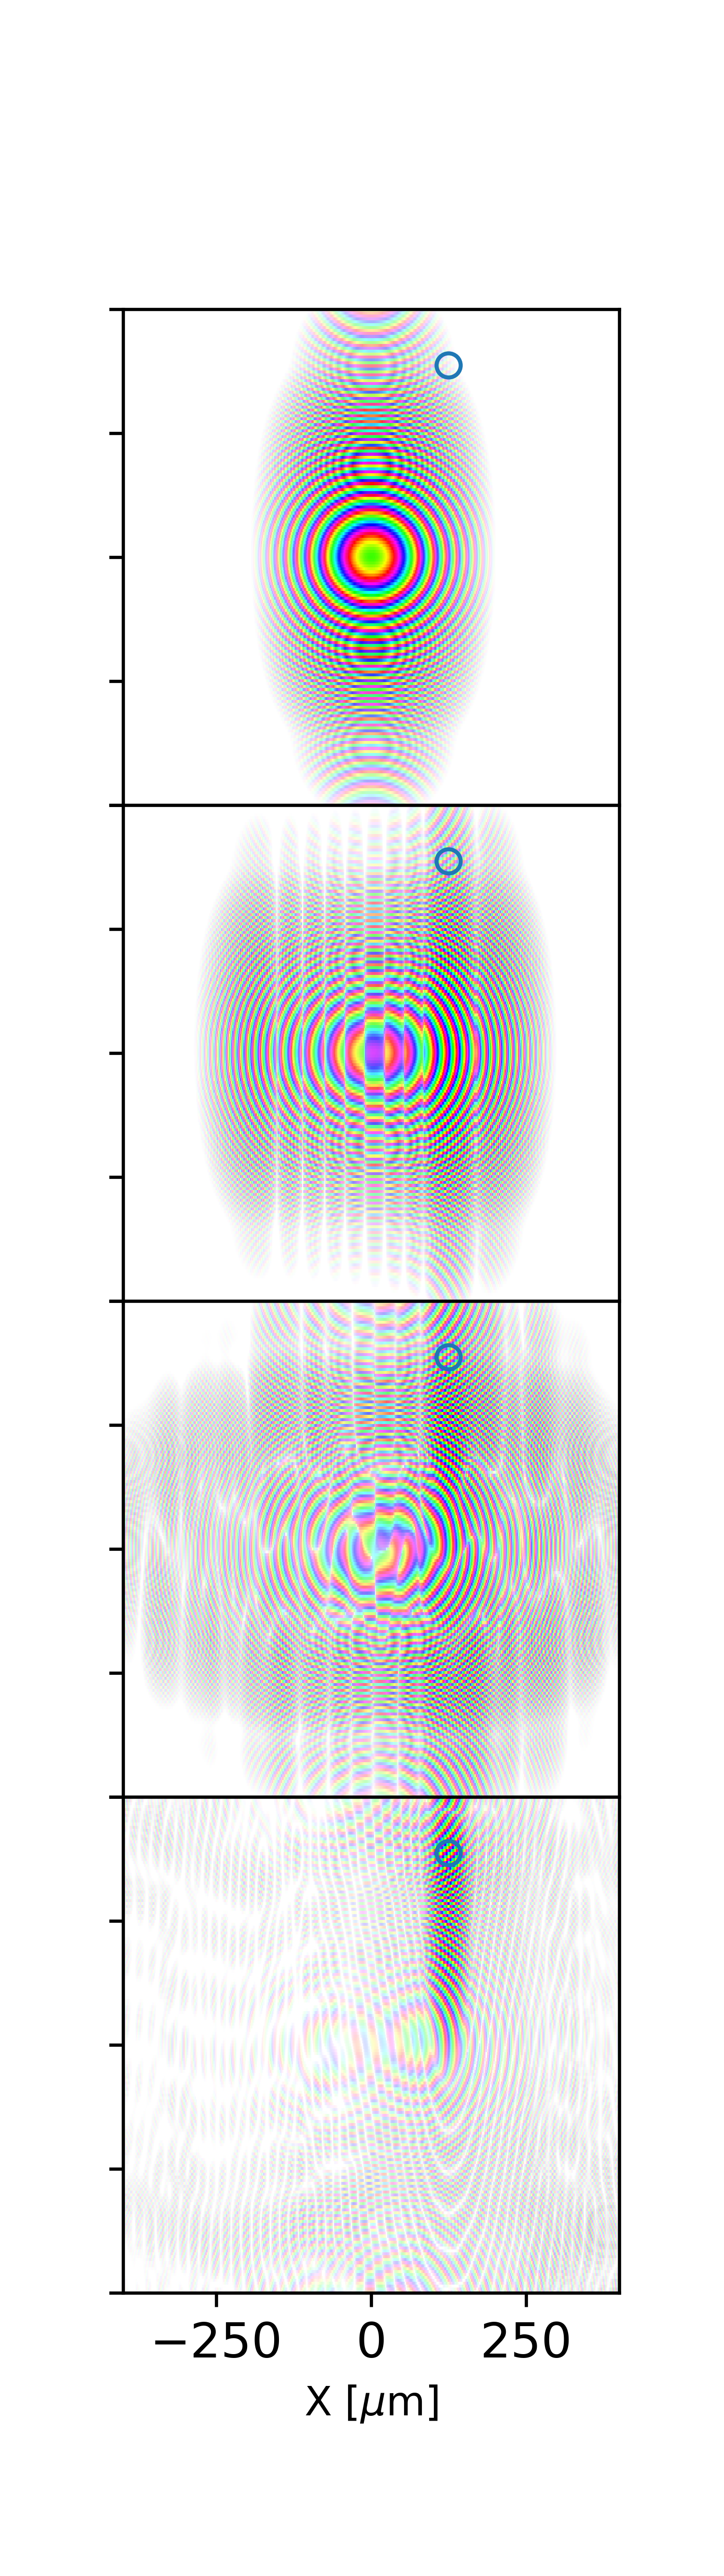
\includegraphics[width=2.75cm]{Figures/vx_id16a_C_propagated.png}
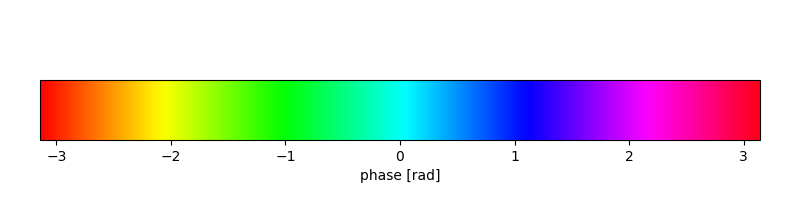
\includegraphics[width=7cm]{Figures/color_bar.png}
\label{points_propagated30}
\end{figure}


The Figure~\ref{pointC_propagated} shows the propagated CSD at various distances (D=1,5,100) at a point C'. Its coordinates are scaled with respect of the coordinates of C' at D=30, such as $(x_{C',D},y_{C',D})=(x_{C',D=30},y_{C',D=30} D / 30.0)$. The results show a much rich structure at short propagation distances (near field), and the image at D=100m looks similar to the corresponding one at D=30m in Fig.~\ref{points_propagated30}. It can be shown that phase maps are very different at D=1m and at D=5m, manifesting that we are in the near field regime.   


\begin{figure}
\caption{Phase as a function of $(x,y)$ of $W(x,y,x_{C'},y_{C'})$ at z=1m (top),5m (middle) and 100m (bottom), when the number $n$ of non-dominant coherent modes is (a, top) 1; (b) 10; (c) 100; (d, bottom) 1000. The brightness of the displayed phase is proportional to $|W(x,y,x_{C'},y_{C'})|$, since CSD phase is not meaningful when $|W(x,y,x_{C'},y_{C'})|$ is negligible.}
C'@1m~~~~~~~~~~~~~~~~~~~~~~~~~~~~C'@5m~~~~~~~~~~~~~~~~~~~~~~~~~~~~C'@100m\\
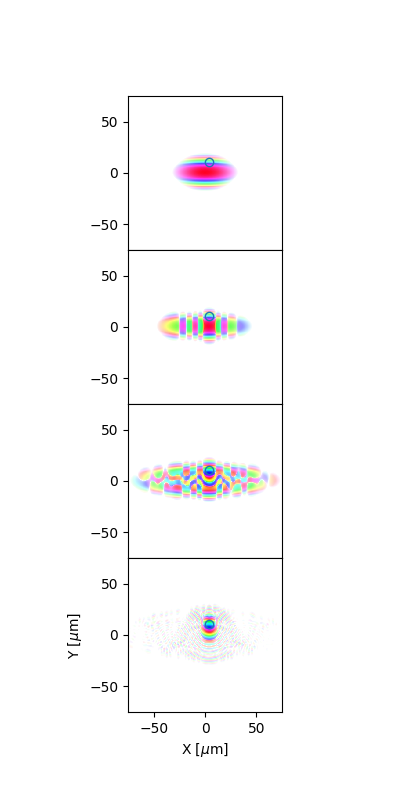
\includegraphics[width=2.75cm]{Figures/vx_id16a_C1_propagated.png}
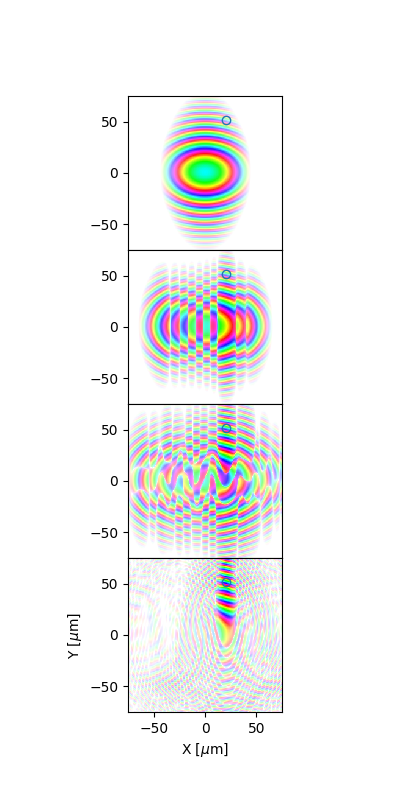
\includegraphics[width=2.75cm]{Figures/vx_id16a_C5_propagated.png}
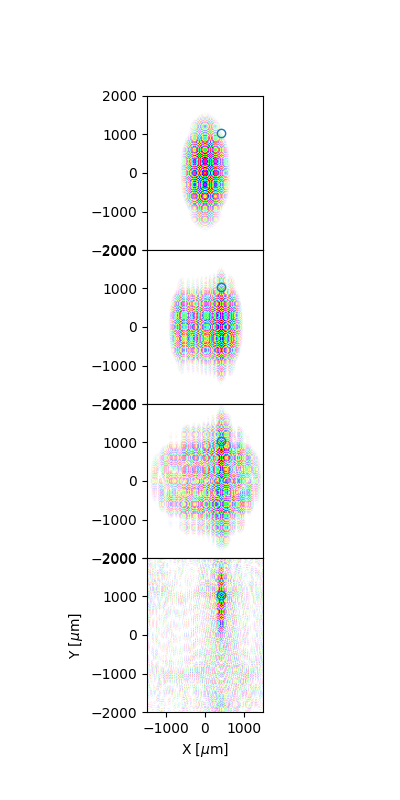
\includegraphics[width=2.75cm]{Figures/vx_id16a_C100_propagated.png}
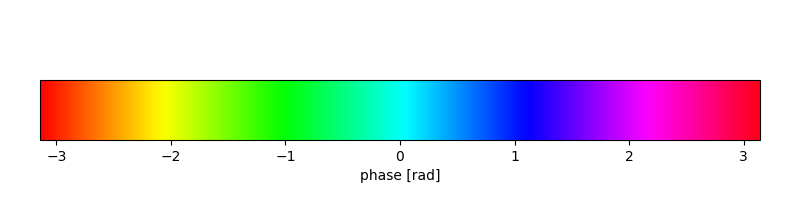
\includegraphics[width=7cm]{Figures/color_bar.png}
\label{pointC_propagated}
\end{figure}

Next we want to see how the phase maps evolve in the neighbourhood of a propagated distance. For that a situation with a map rich in vortices with resolution that allows to study the variations. Ideally the maps for D=1m n=100 could be selected, but we preferred to go to longer distance (position where it would be feasible to have a measurement) and reduce the maximum mode. Selecting D=5$\pm$1 m and n=20 we "scanned" the phase map along 1m keeping fixed the point C'. Fig.~\ref{neighbour} shows the result. 


\begin{figure}
\caption{Phase as a function of $(x,y)$ of $W(x,y,x_{C'},y_{C'})$ at different distances close to D=5$\pm$1 m, when the number $n$ of non-dominant coherent modes is 10 (top), 20 (middle) and 100 (bottom). The brightness of the displayed phase is proportional to $|W(x,y,x_{C'},y_{C'})|$, since CSD phase is not meaningful when $|W(x,y,x_{C'},y_{C'})|$ is negligible.}
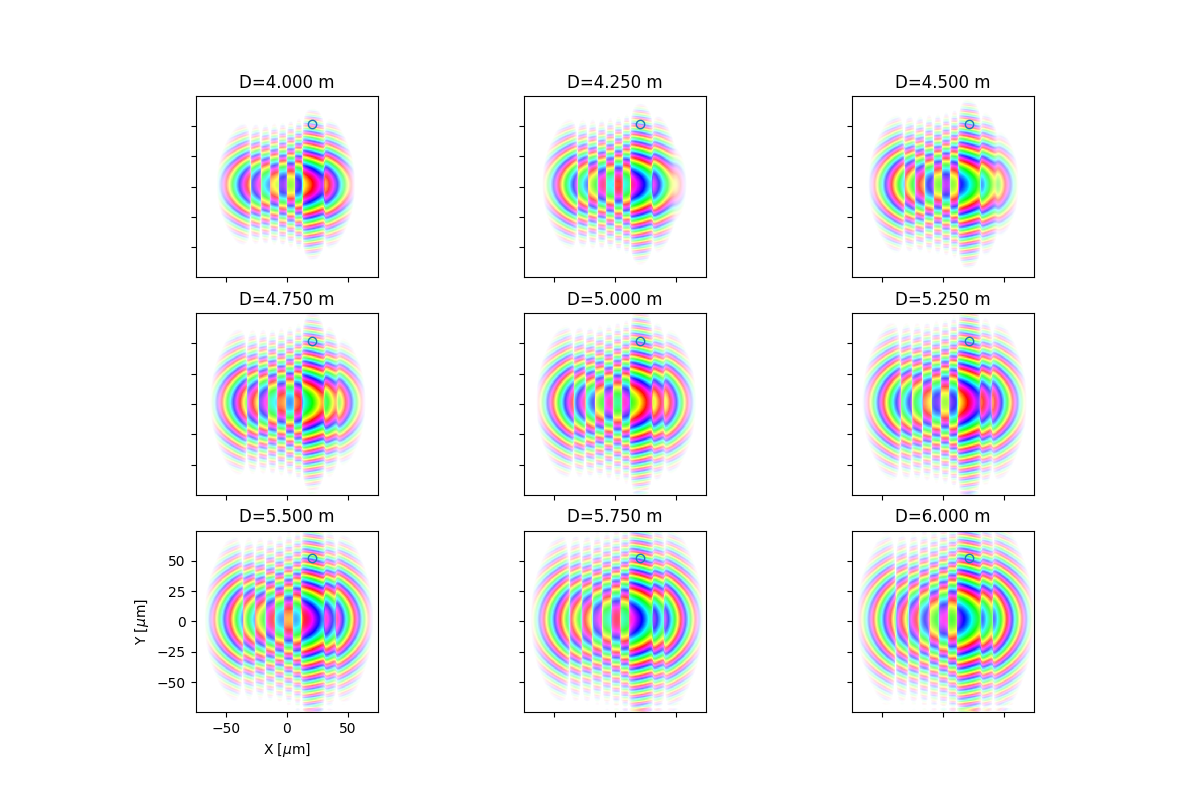
\includegraphics[width=9cm]{Figures/vx_id16a_C5_propagated_neighbour_mode0009.png}
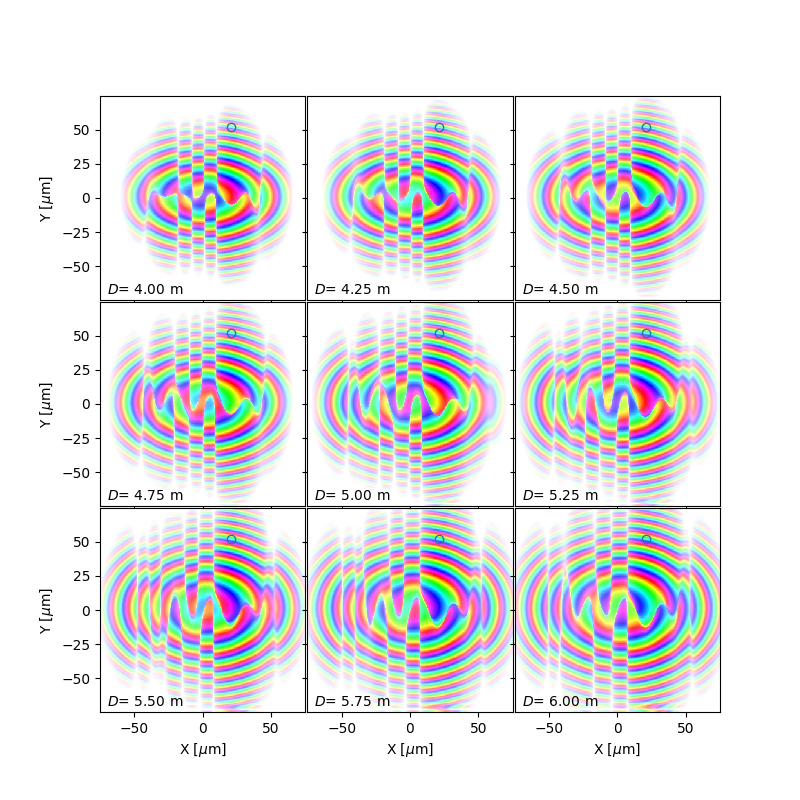
\includegraphics[width=9cm]{Figures/vx_id16a_C5_propagated_neighbour_mode0019.png}
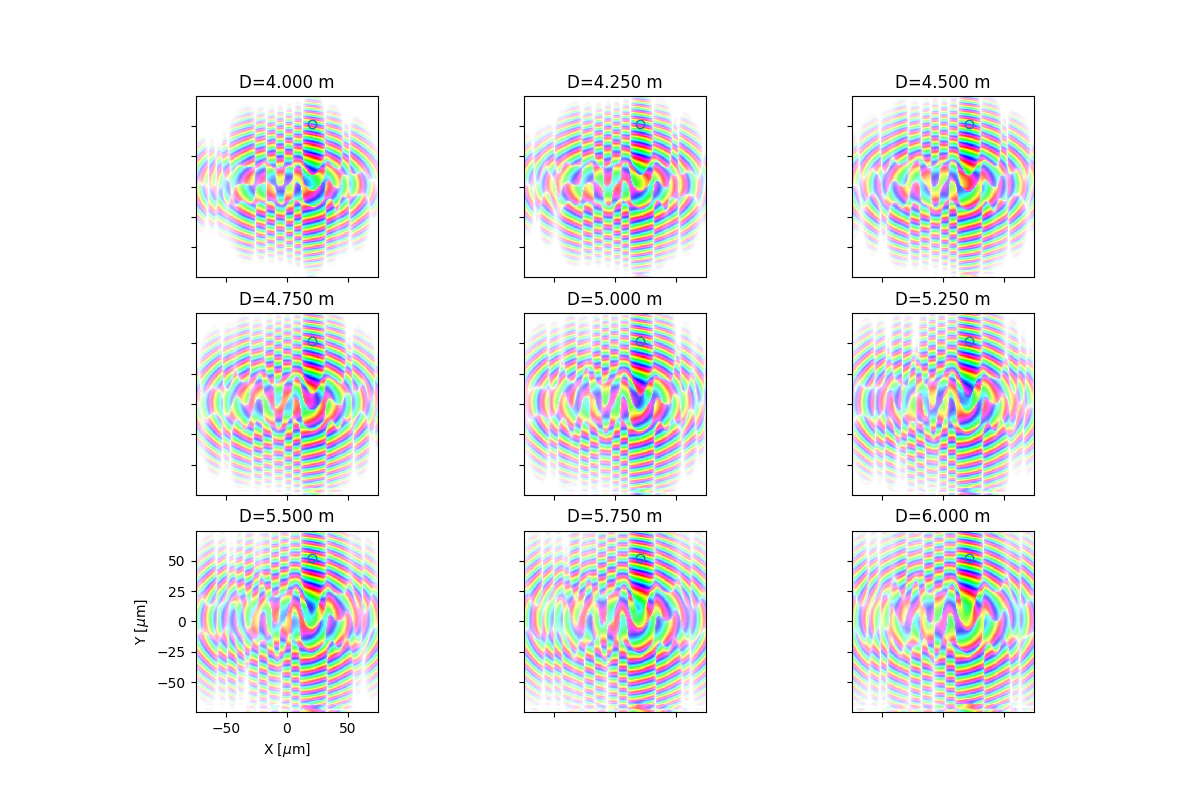
\includegraphics[width=9cm]{Figures/vx_id16a_C5_propagated_neighbour_mode0099.png}
\label{neighbour}
\end{figure}


Next, we want to simulate a sort of Young experiment by placing two circular apertures in the plane to where the CSD has been propagated (5 m downstream from the source). These apertures are at points (xD,yD)=(-10$\mu m$,-25$\mu m$) and its opposite (xE,yE)=(10$\mu m$,25$\mu m$). The slits apertures are closed to 3.6 and 3$\mu m$ for points D and E, respectively. The radiation thet goes through the apertures is propagated 30m downstream the plane with the apertures. At the image plane a screen is placed to record the intensity. When the apertures are illuminated by a mostly coherent source an interference pattern with fringes is produced. Fig.~\ref{young} (top) shows the interferece pattern produced by the CSD calculating using only the zeroth mode (complete coherence). It can be observed a strong visibility or contrast in the fringes, as expected for a coherent source. Adding coherent modes in the construction of the CSD will reduce progressively the visibility (see pattern up to mode 3 in Fig.~\ref{young}). However, adding the mode index 4 in the construction of the CSD will drastically reduce the contrast in the fringes, because now the CSD presents a vortex in E. The mode 5 will not modify substantially the situation, but mode 6 pushes the vortex outside the aperture E recovering some visibility. This situation repeats several times as one increses the number of modes that contribute to the CSD. For example, the CSD built with modes up to 18 does not present a vortex in E, but up to mode 20 does (Fig.~\ref{young2}). Increasing the number of modes used for building the CSD makes an the beam less and less coherent, and the fringes visibility is then lost, see for example the case of CSD up to the 99th mode in Fig.~\ref{young2}. 

It is interesting to remark that although this procedure of adding modes to built the CSD is an artificial way to study the visibility depending on the coherence, in a real situation of a synchrotron beamline the beamline optics play a similar role. In a beamline some optical elements (ideal reflectors, ideal focusing elements) do not alter the occupation spectrum of the modes. They are non-absorbing or conservative elements. However, if an optical element remove photons from the beam, or ``cuts'' intensity, then its effect is different on the different modes. The new transformed ``modes'' can be used to build the CSD, but they cannot be considered coherence modes as they are not an orthonormal basis for expanding the CSD. But a new coherent mode decomposition can be done on the transmitted CSD. In the case of slits or pinholes centerd in the middle of the beam, the lower modes that are well localised near the center of the beam axis will propagate, whereas the higher modes (extended far from the center) will be absorbed. This will produce a push of the occupation spectrum to the lower modes with a resulting increase of coherence fraction (and obviously a decrease of the spectral density or total intensity).     

\begin{figure}
\caption{On the left, the phase of $W(x,y,x_{D},y_{D})$ is represented. The circles represent the position of apertures at D (red) and E (black) used for a Young-type virtual experiment. On the right the interference pattern produced by propagating the radiation 30 m downstream from the plane containing the apertures. Strictly speaking, the Spectral Density obtained from the propagated CSD. From top to bottom, the number of coherent modes used to build the CSD is varied (1,4,5 and 7).}
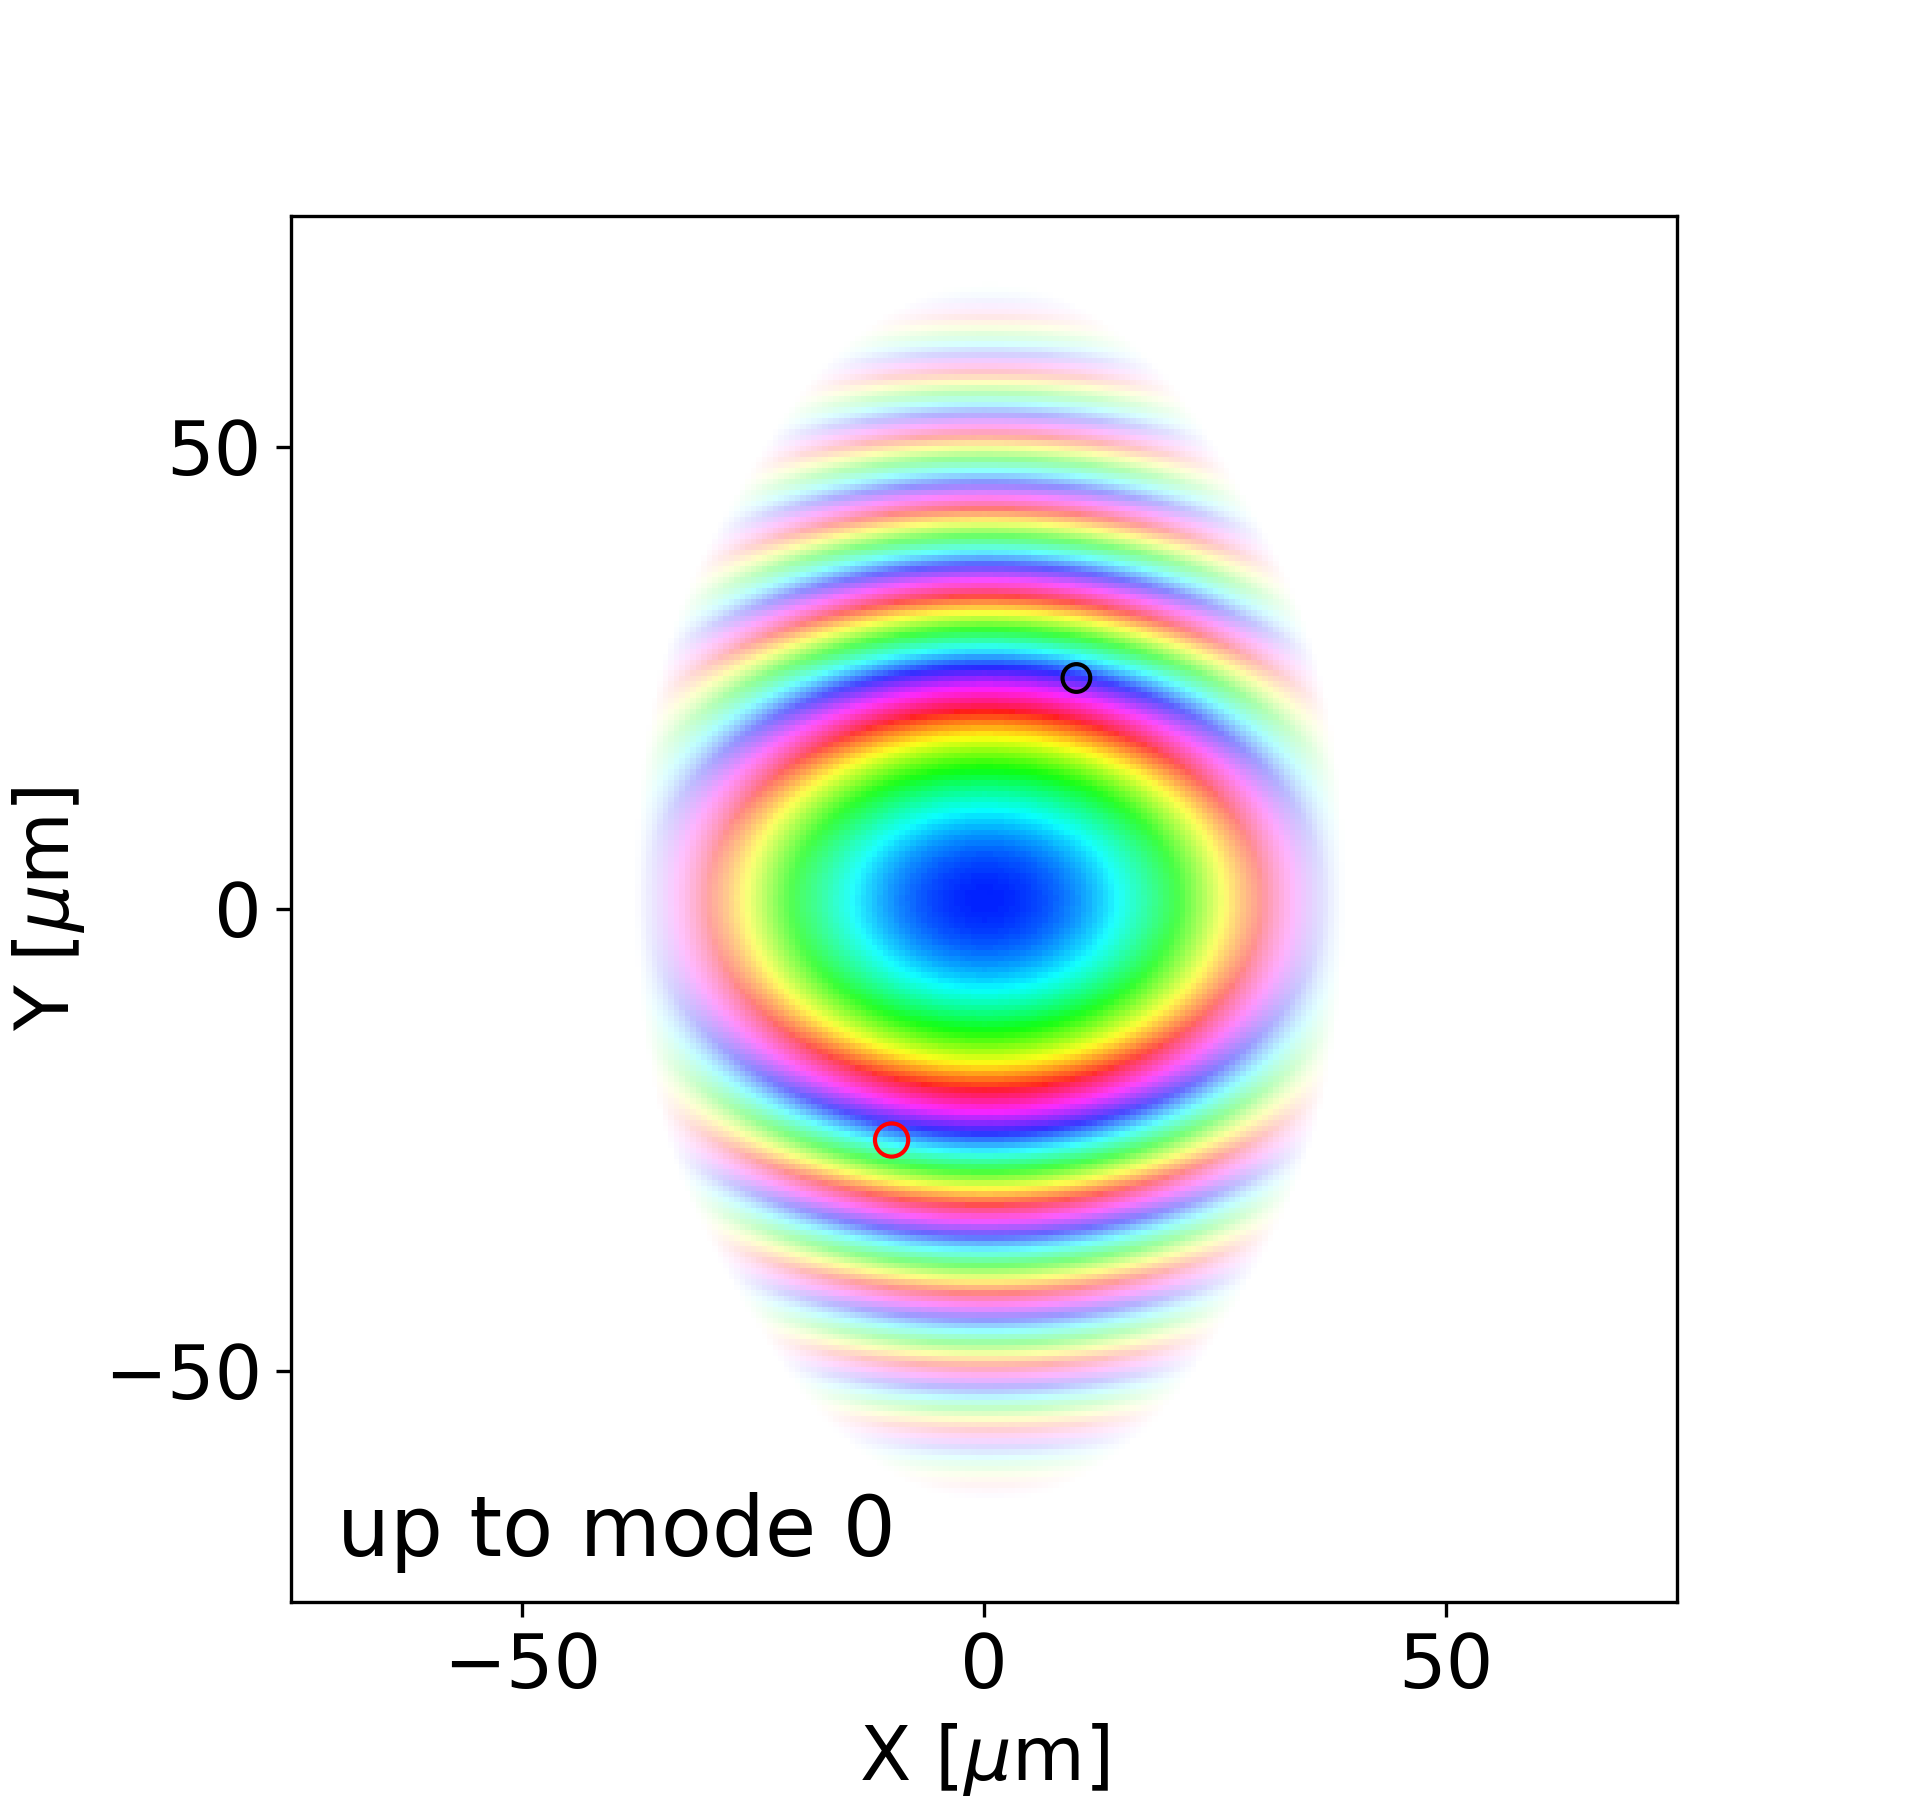
\includegraphics[width=4cm]{Figures/interference_D_uptomode0000_csd.png}
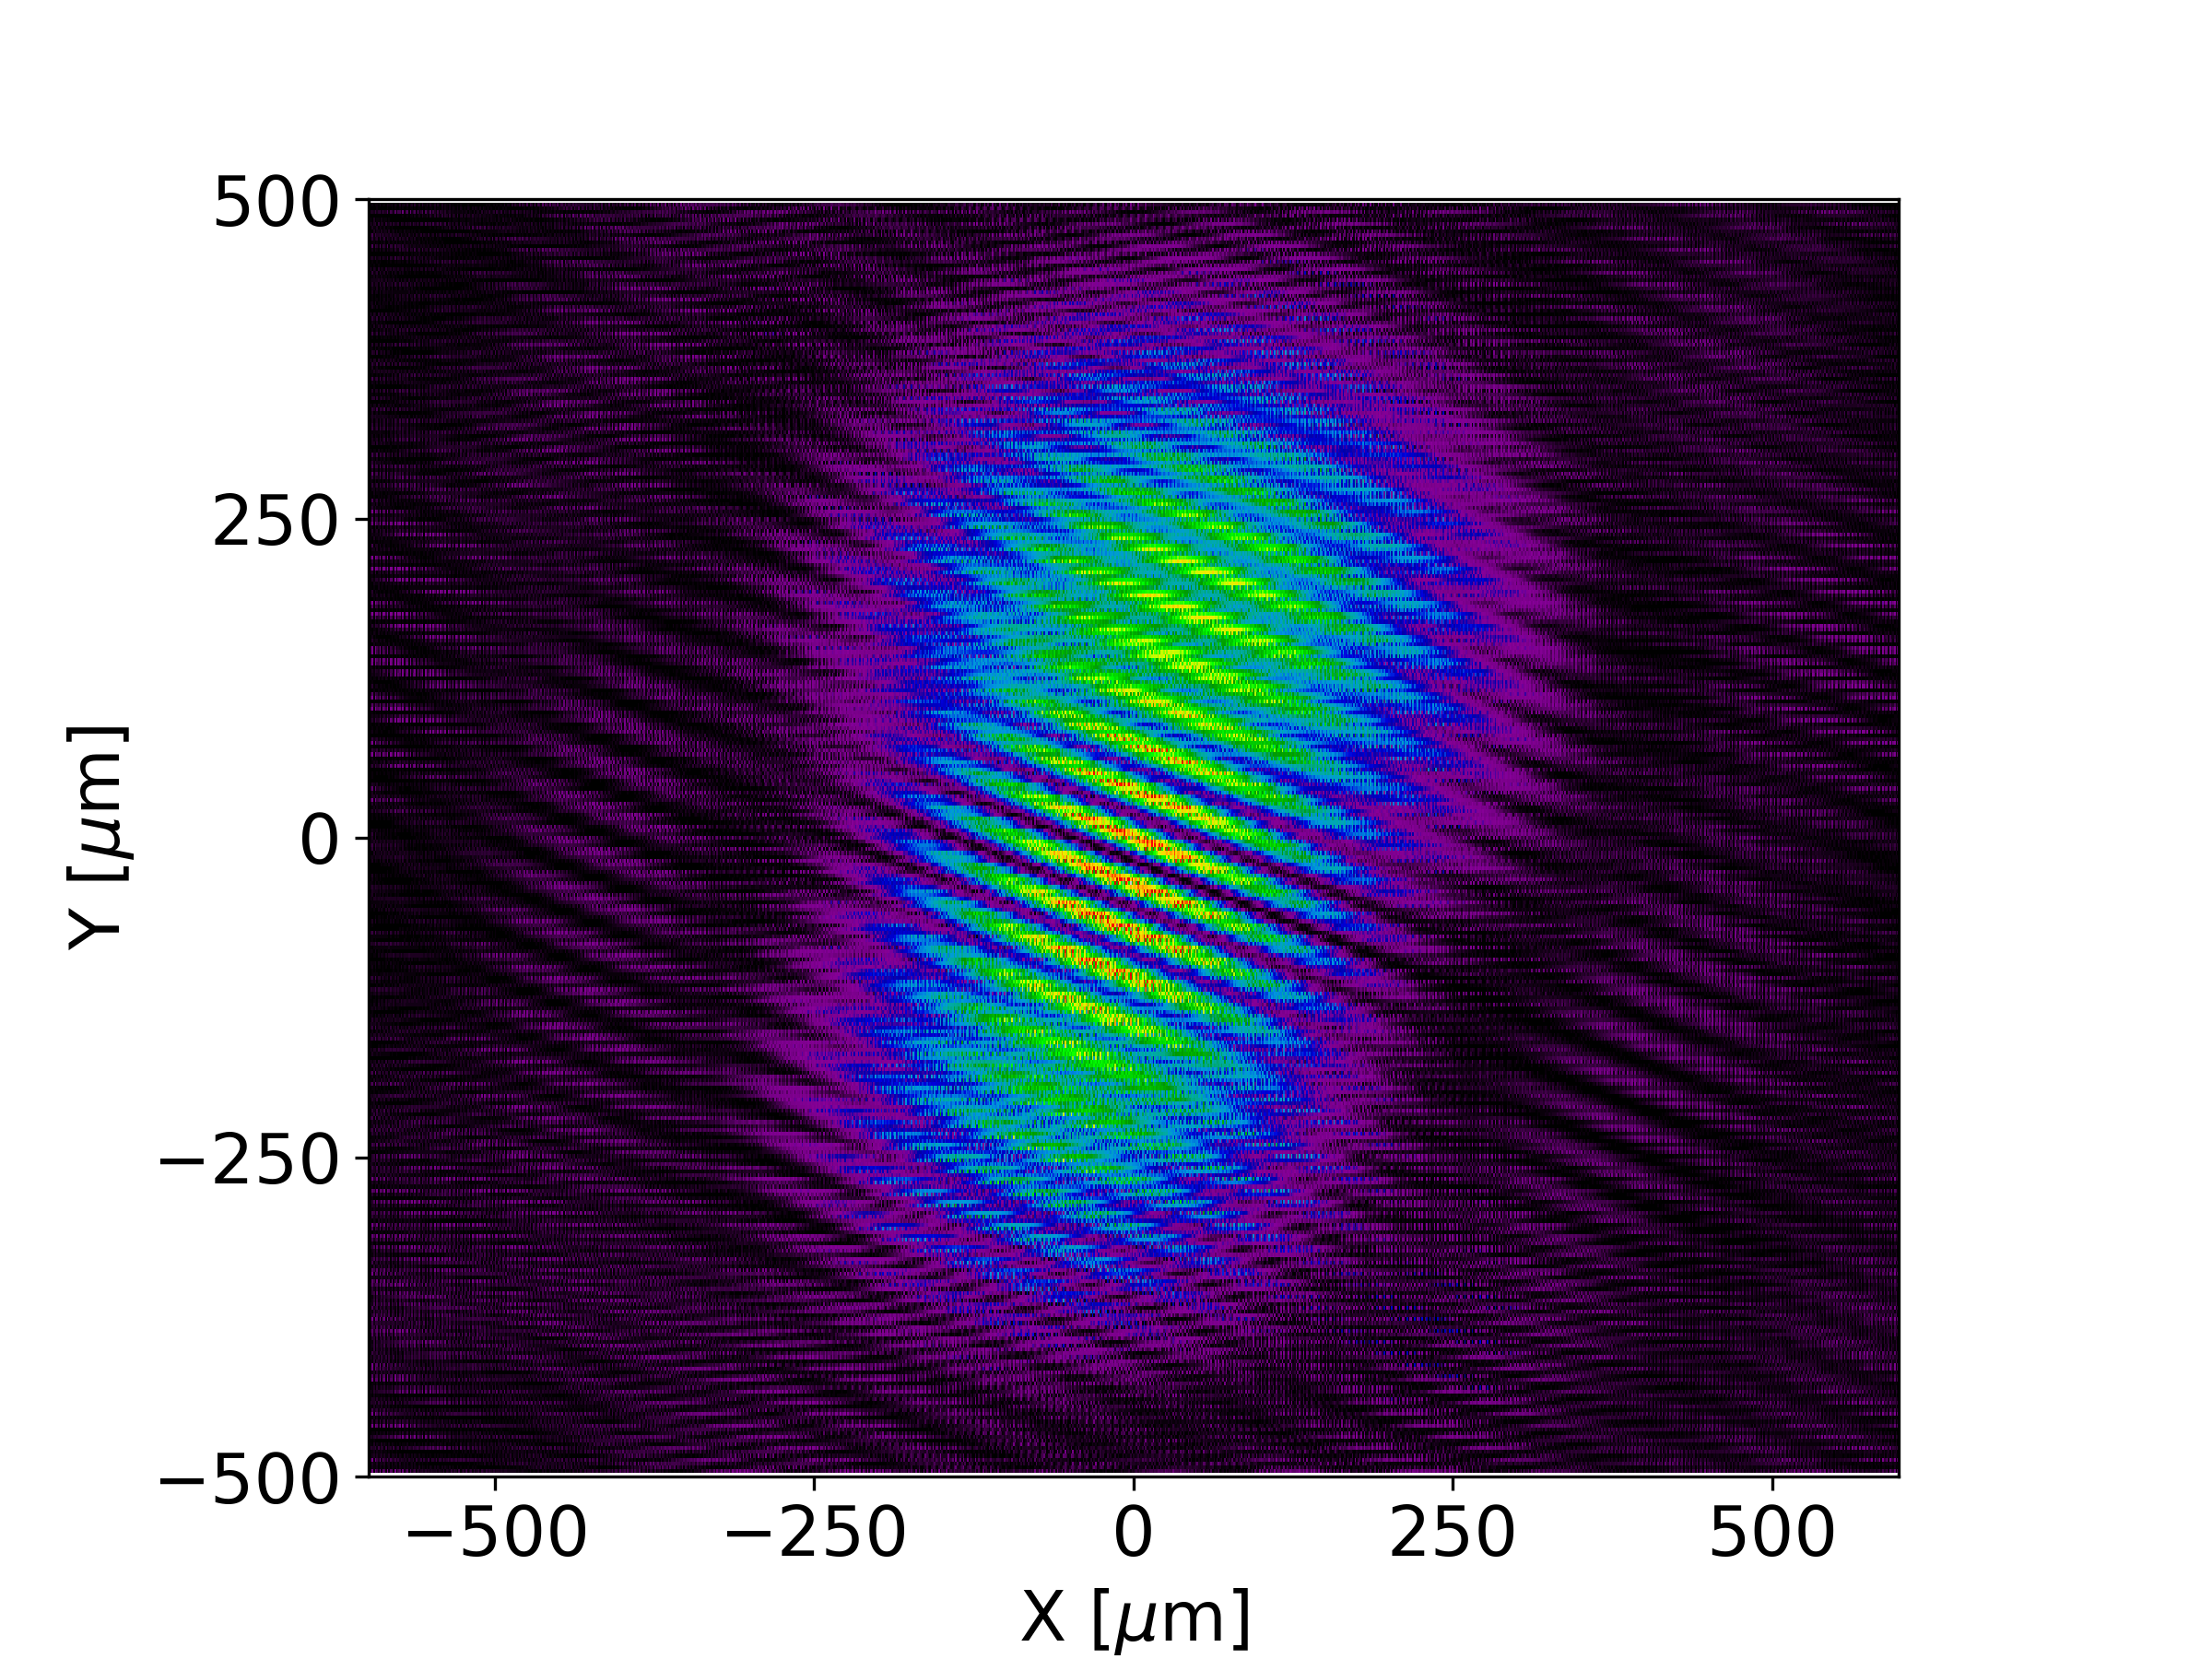
\includegraphics[width=4cm]{Figures/interference_D_uptomode0000_pattern.png}

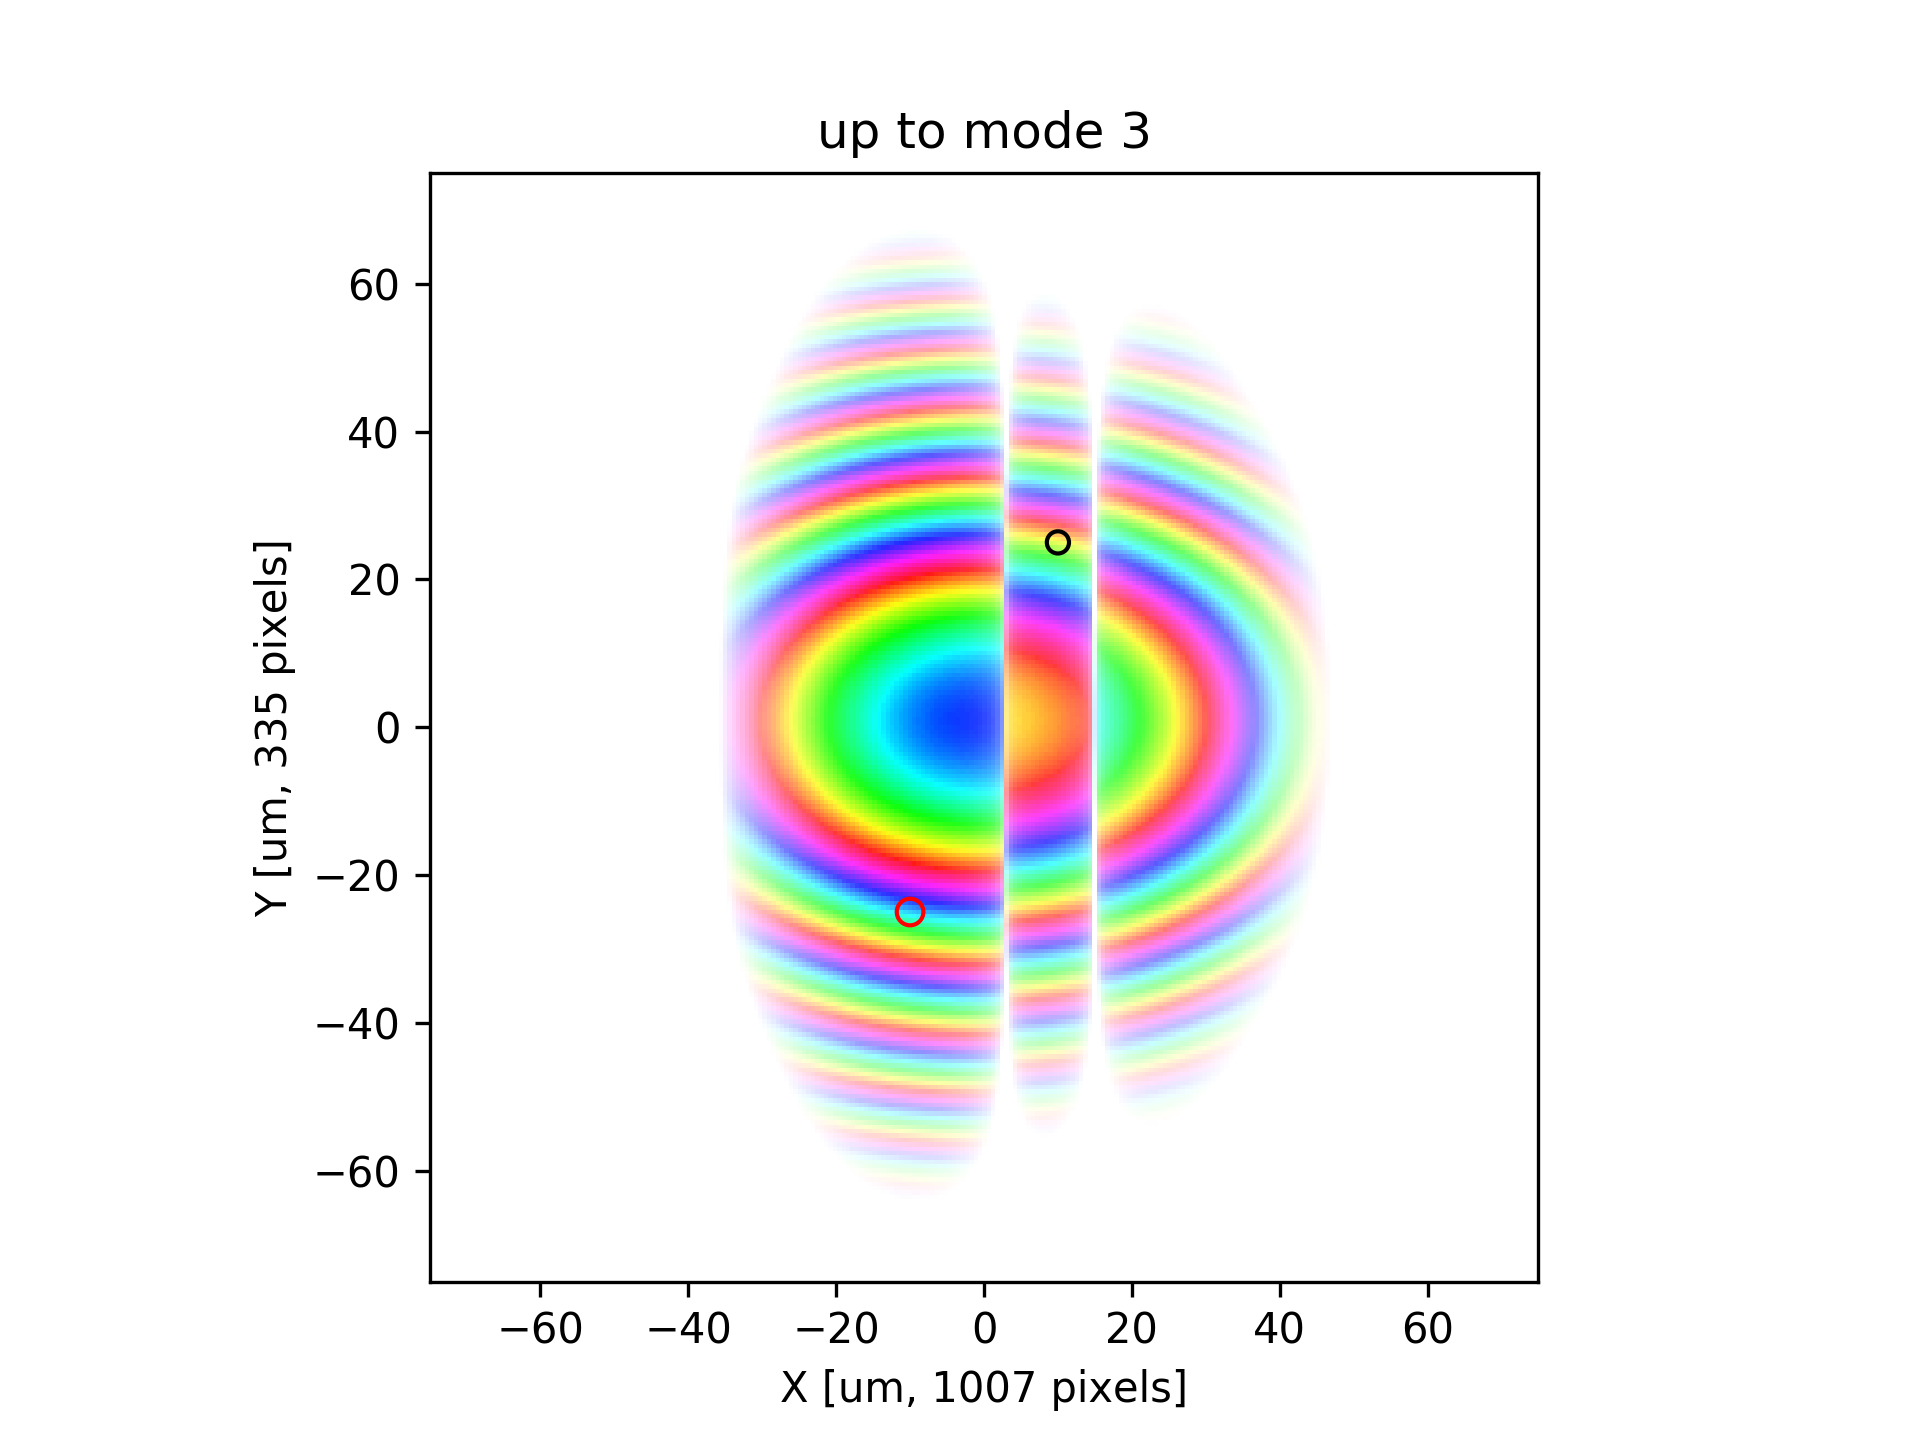
\includegraphics[width=4cm]{Figures/interference_D_uptomode0003_csd.png}
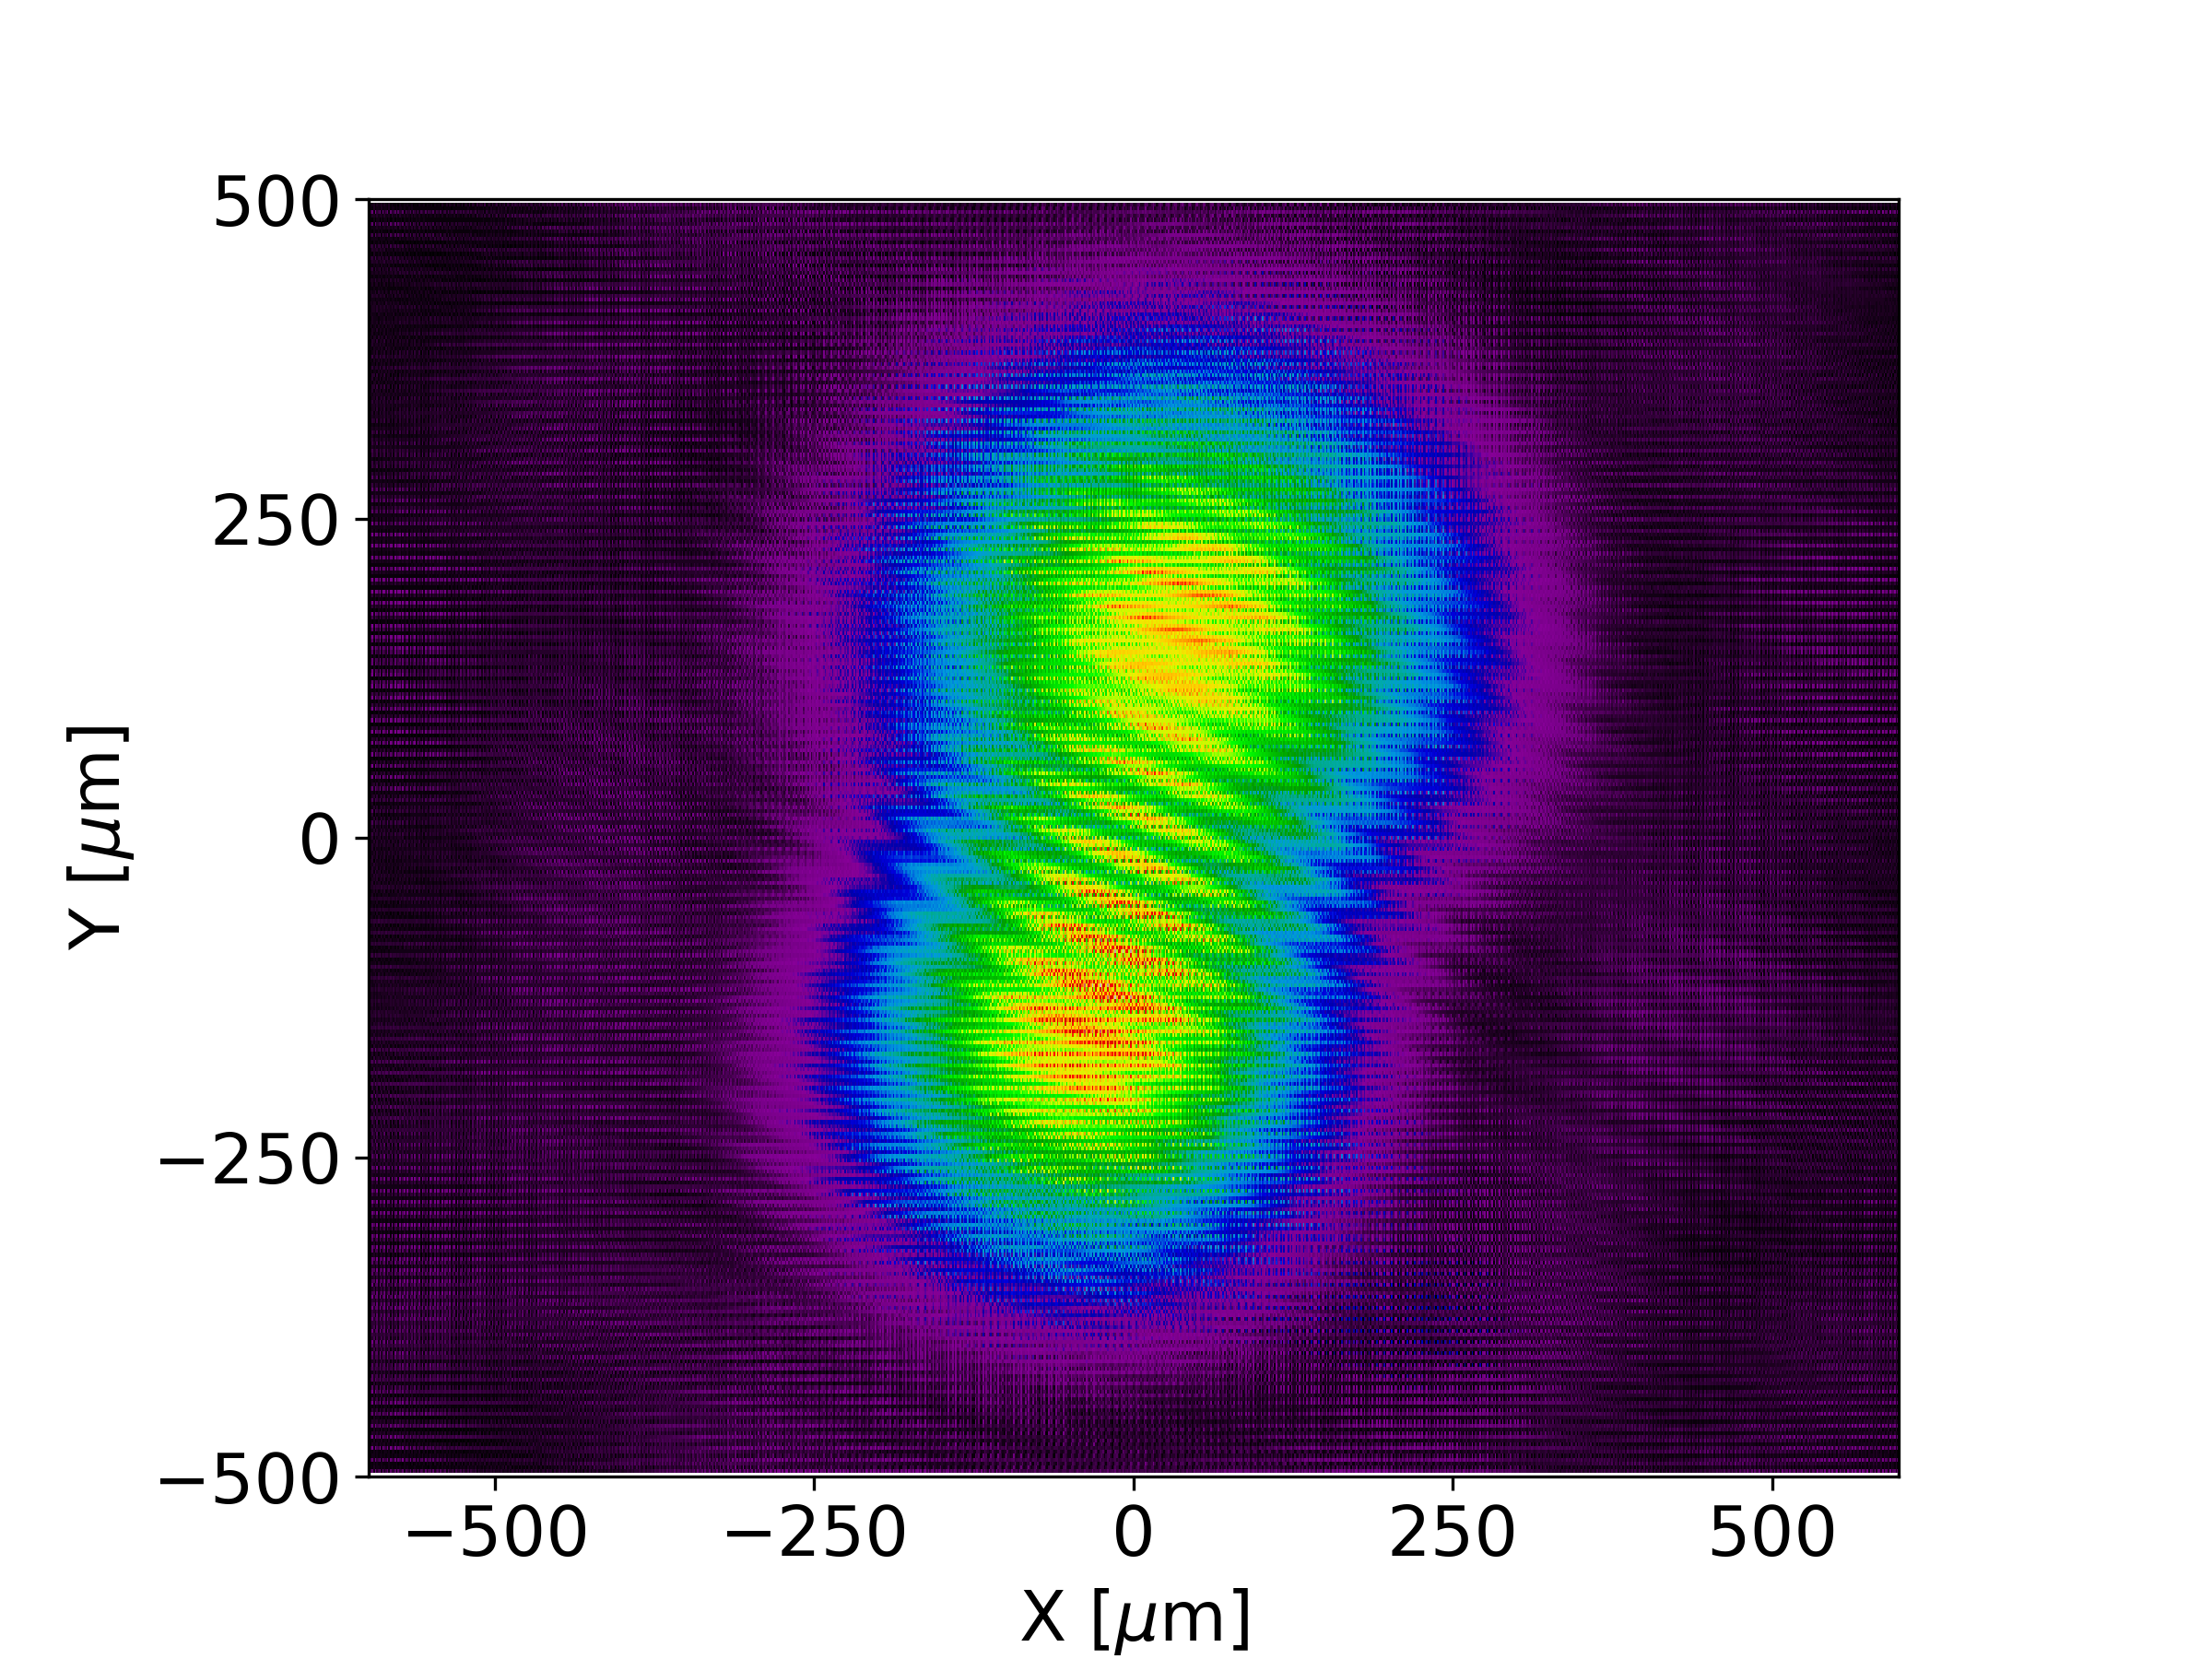
\includegraphics[width=4cm]{Figures/interference_D_uptomode0003_pattern.png}

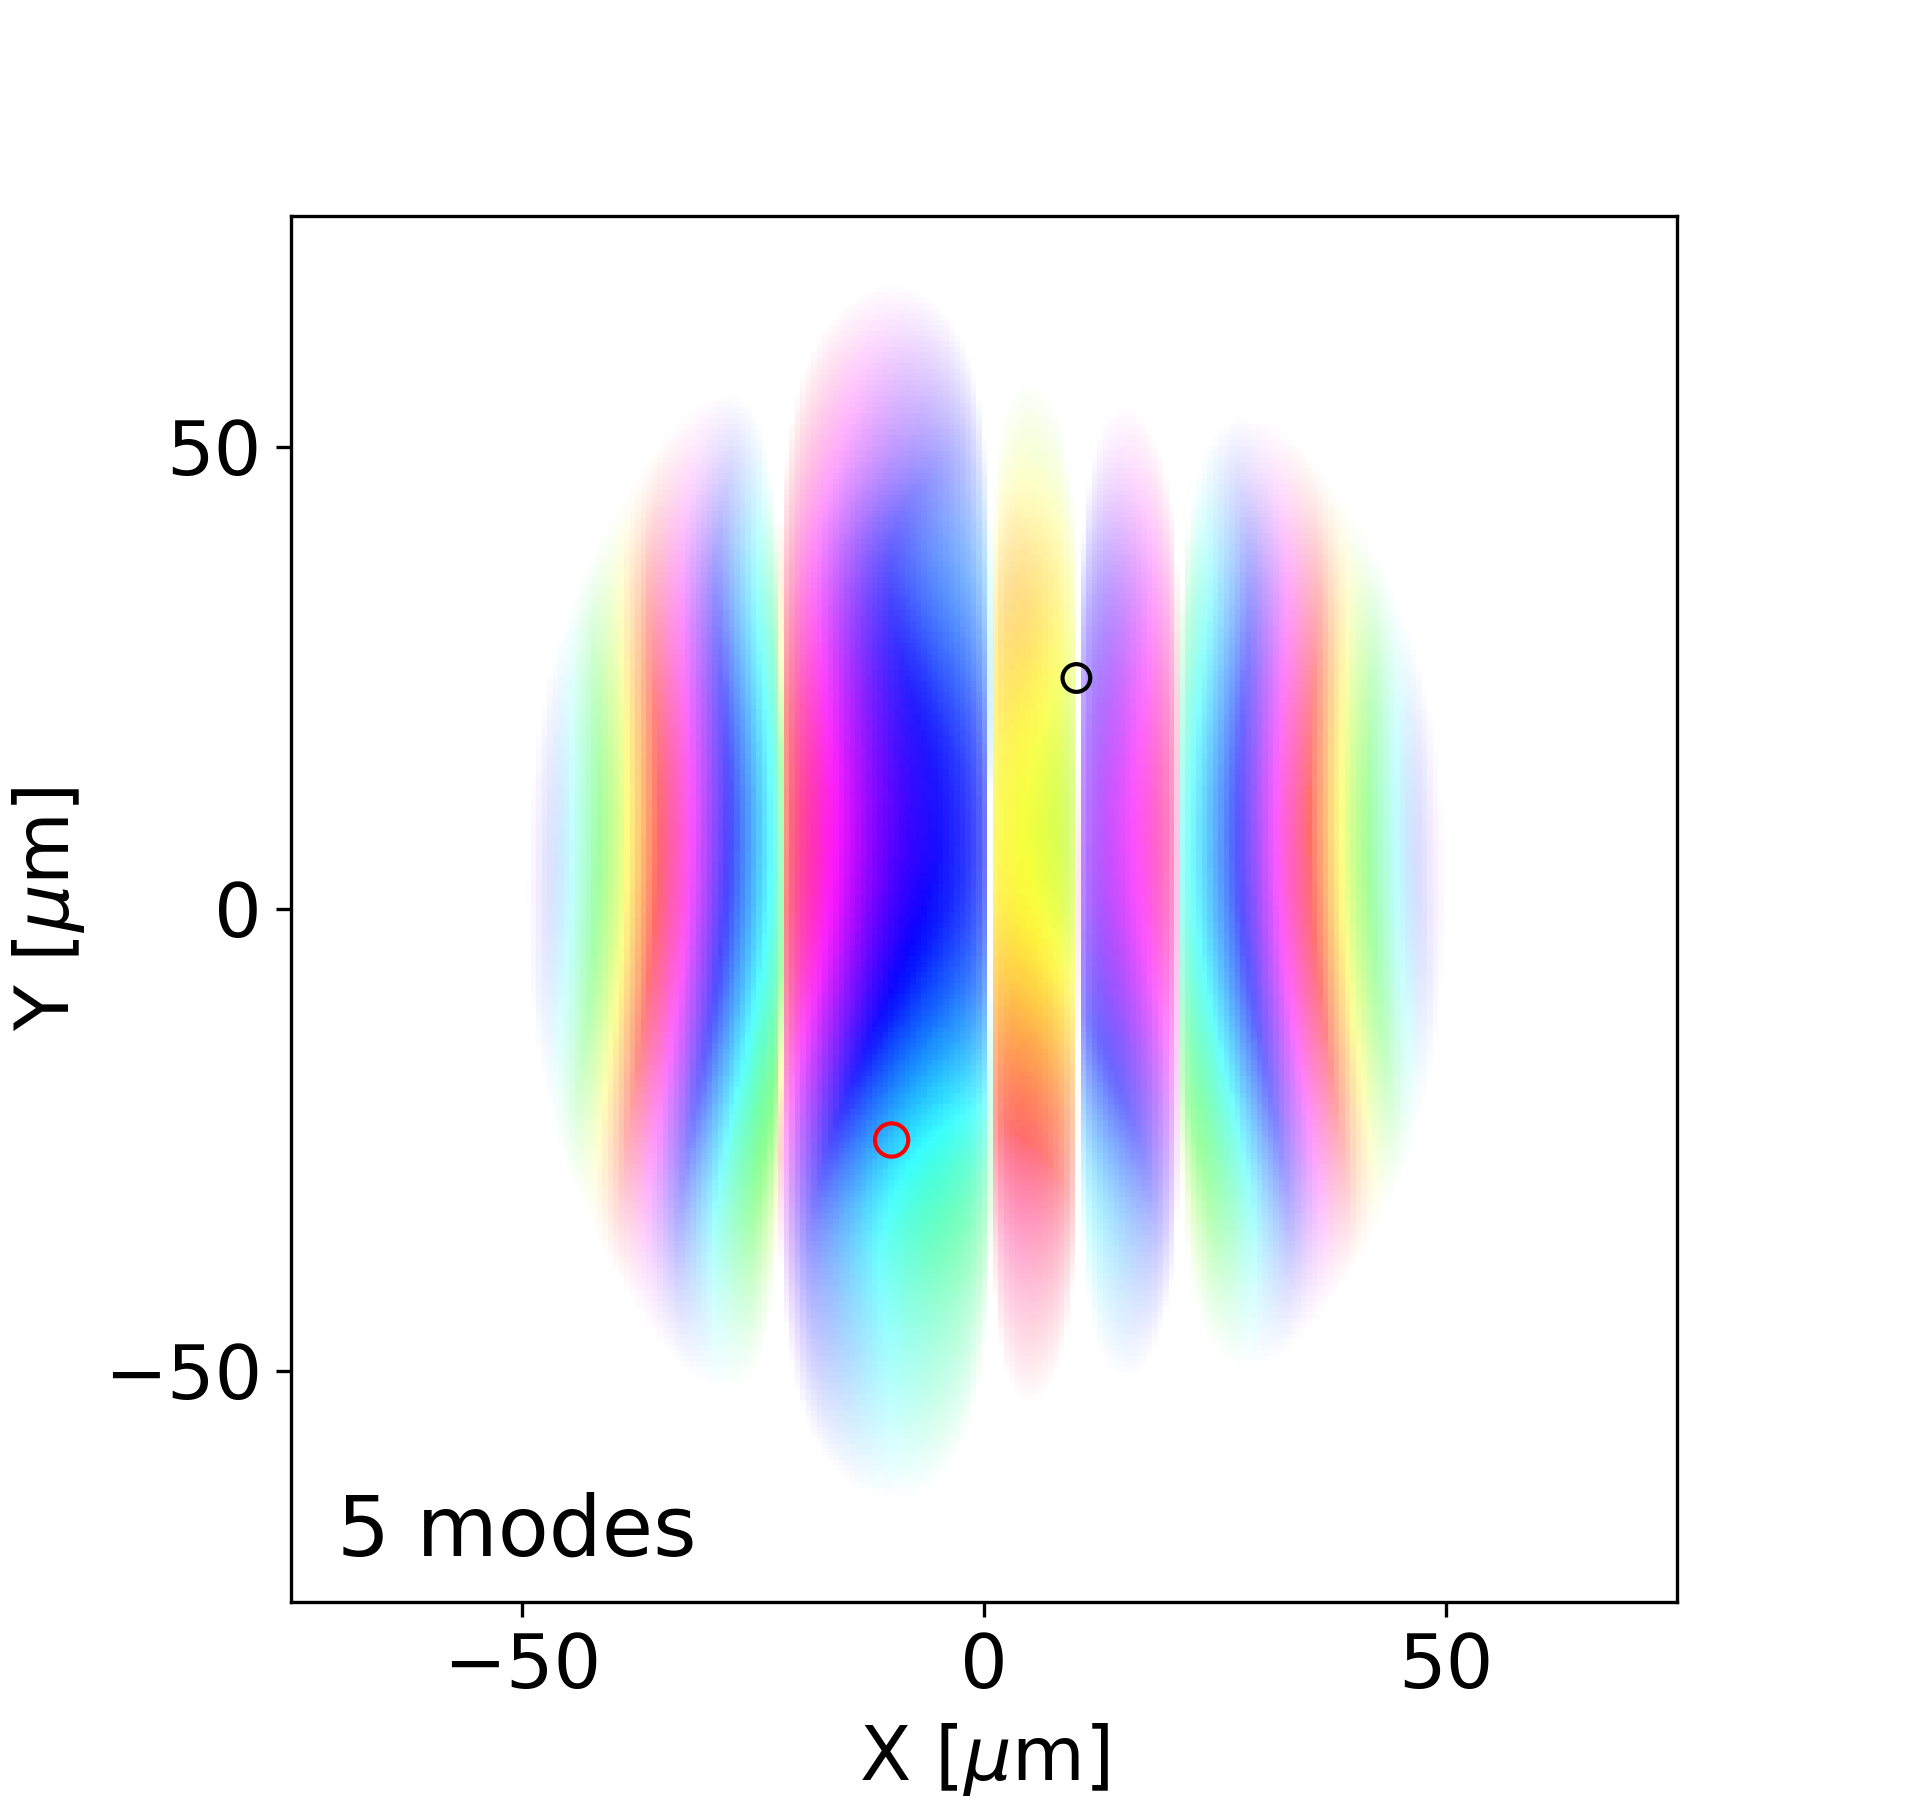
\includegraphics[width=4cm]{Figures/interference_D_uptomode0004_csd.png}
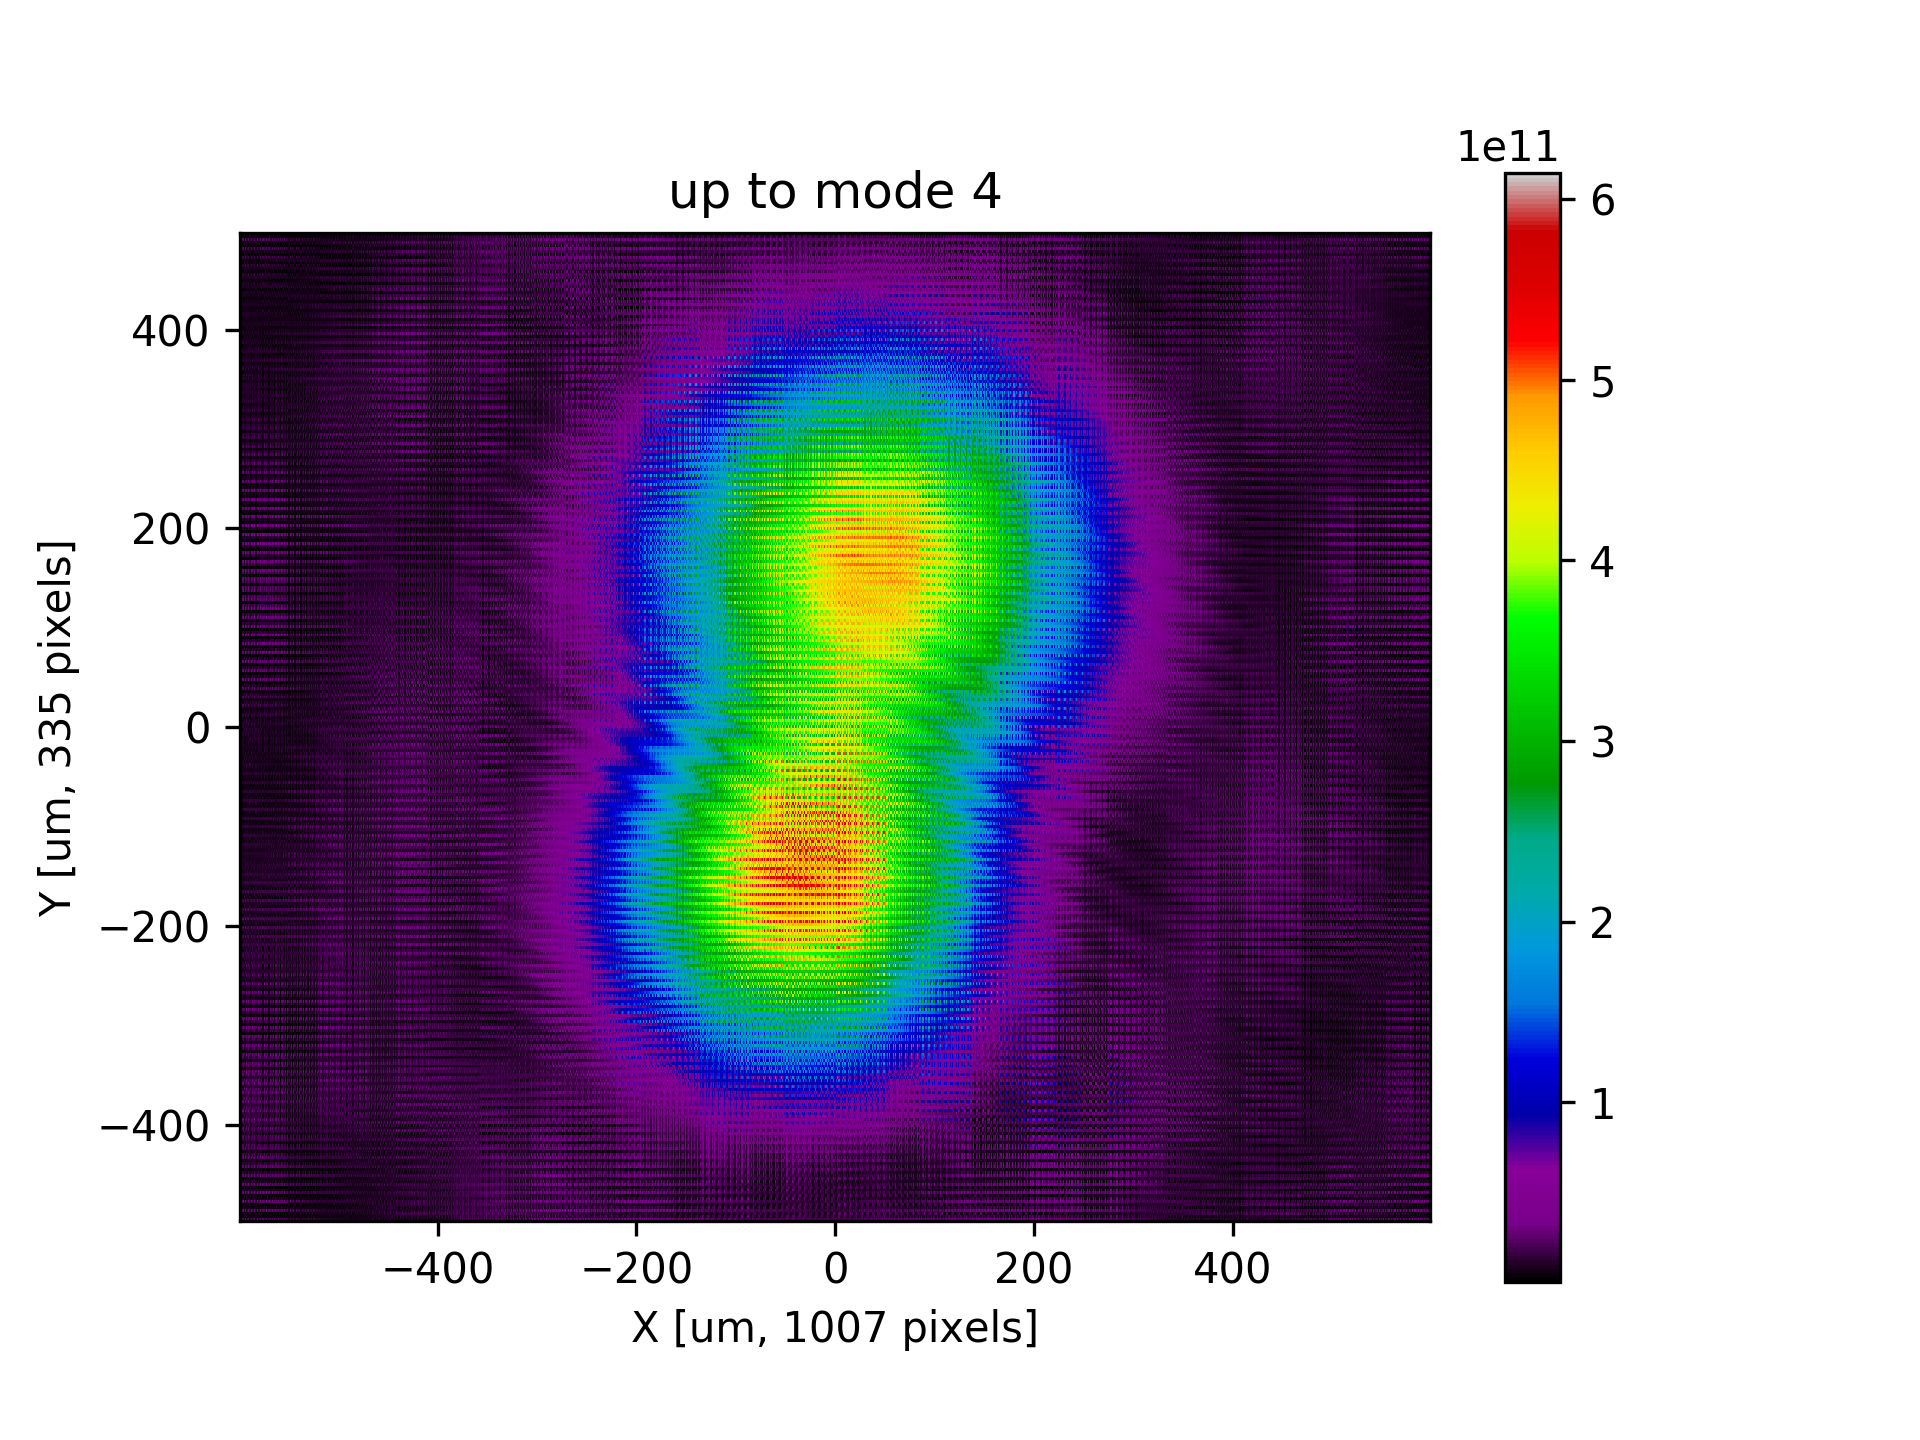
\includegraphics[width=4cm]{Figures/interference_D_uptomode0004_pattern.png}

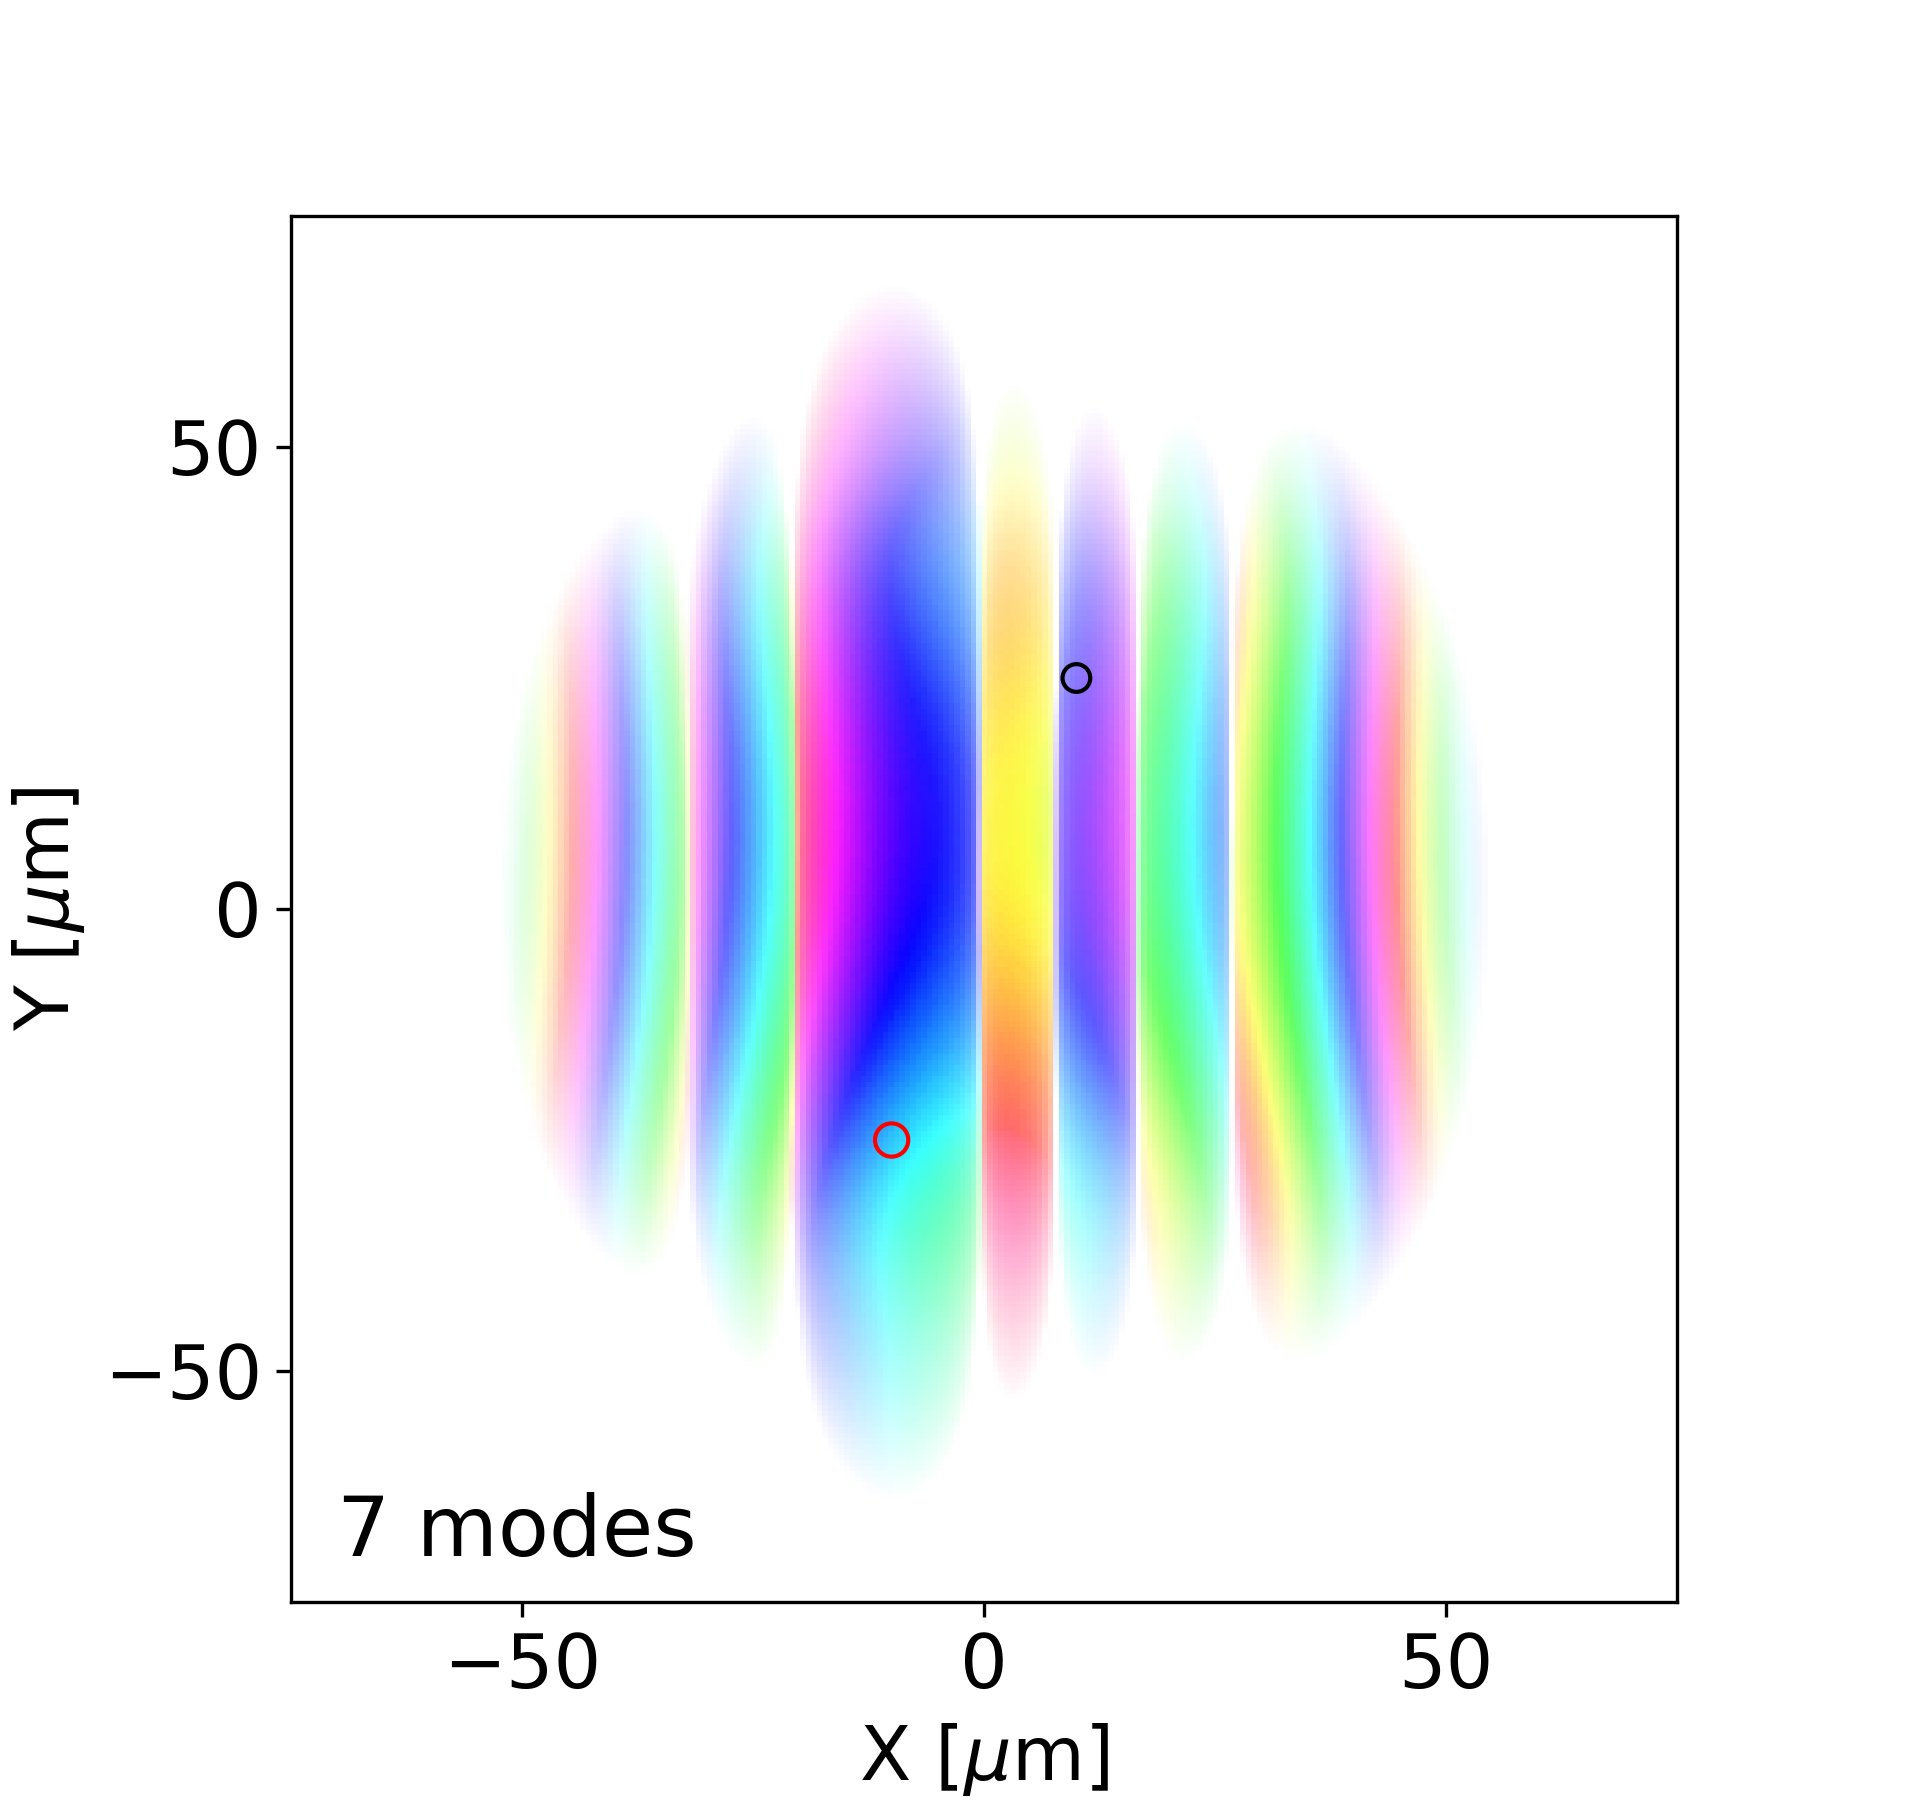
\includegraphics[width=4cm]{Figures/interference_D_uptomode0006_csd.png}
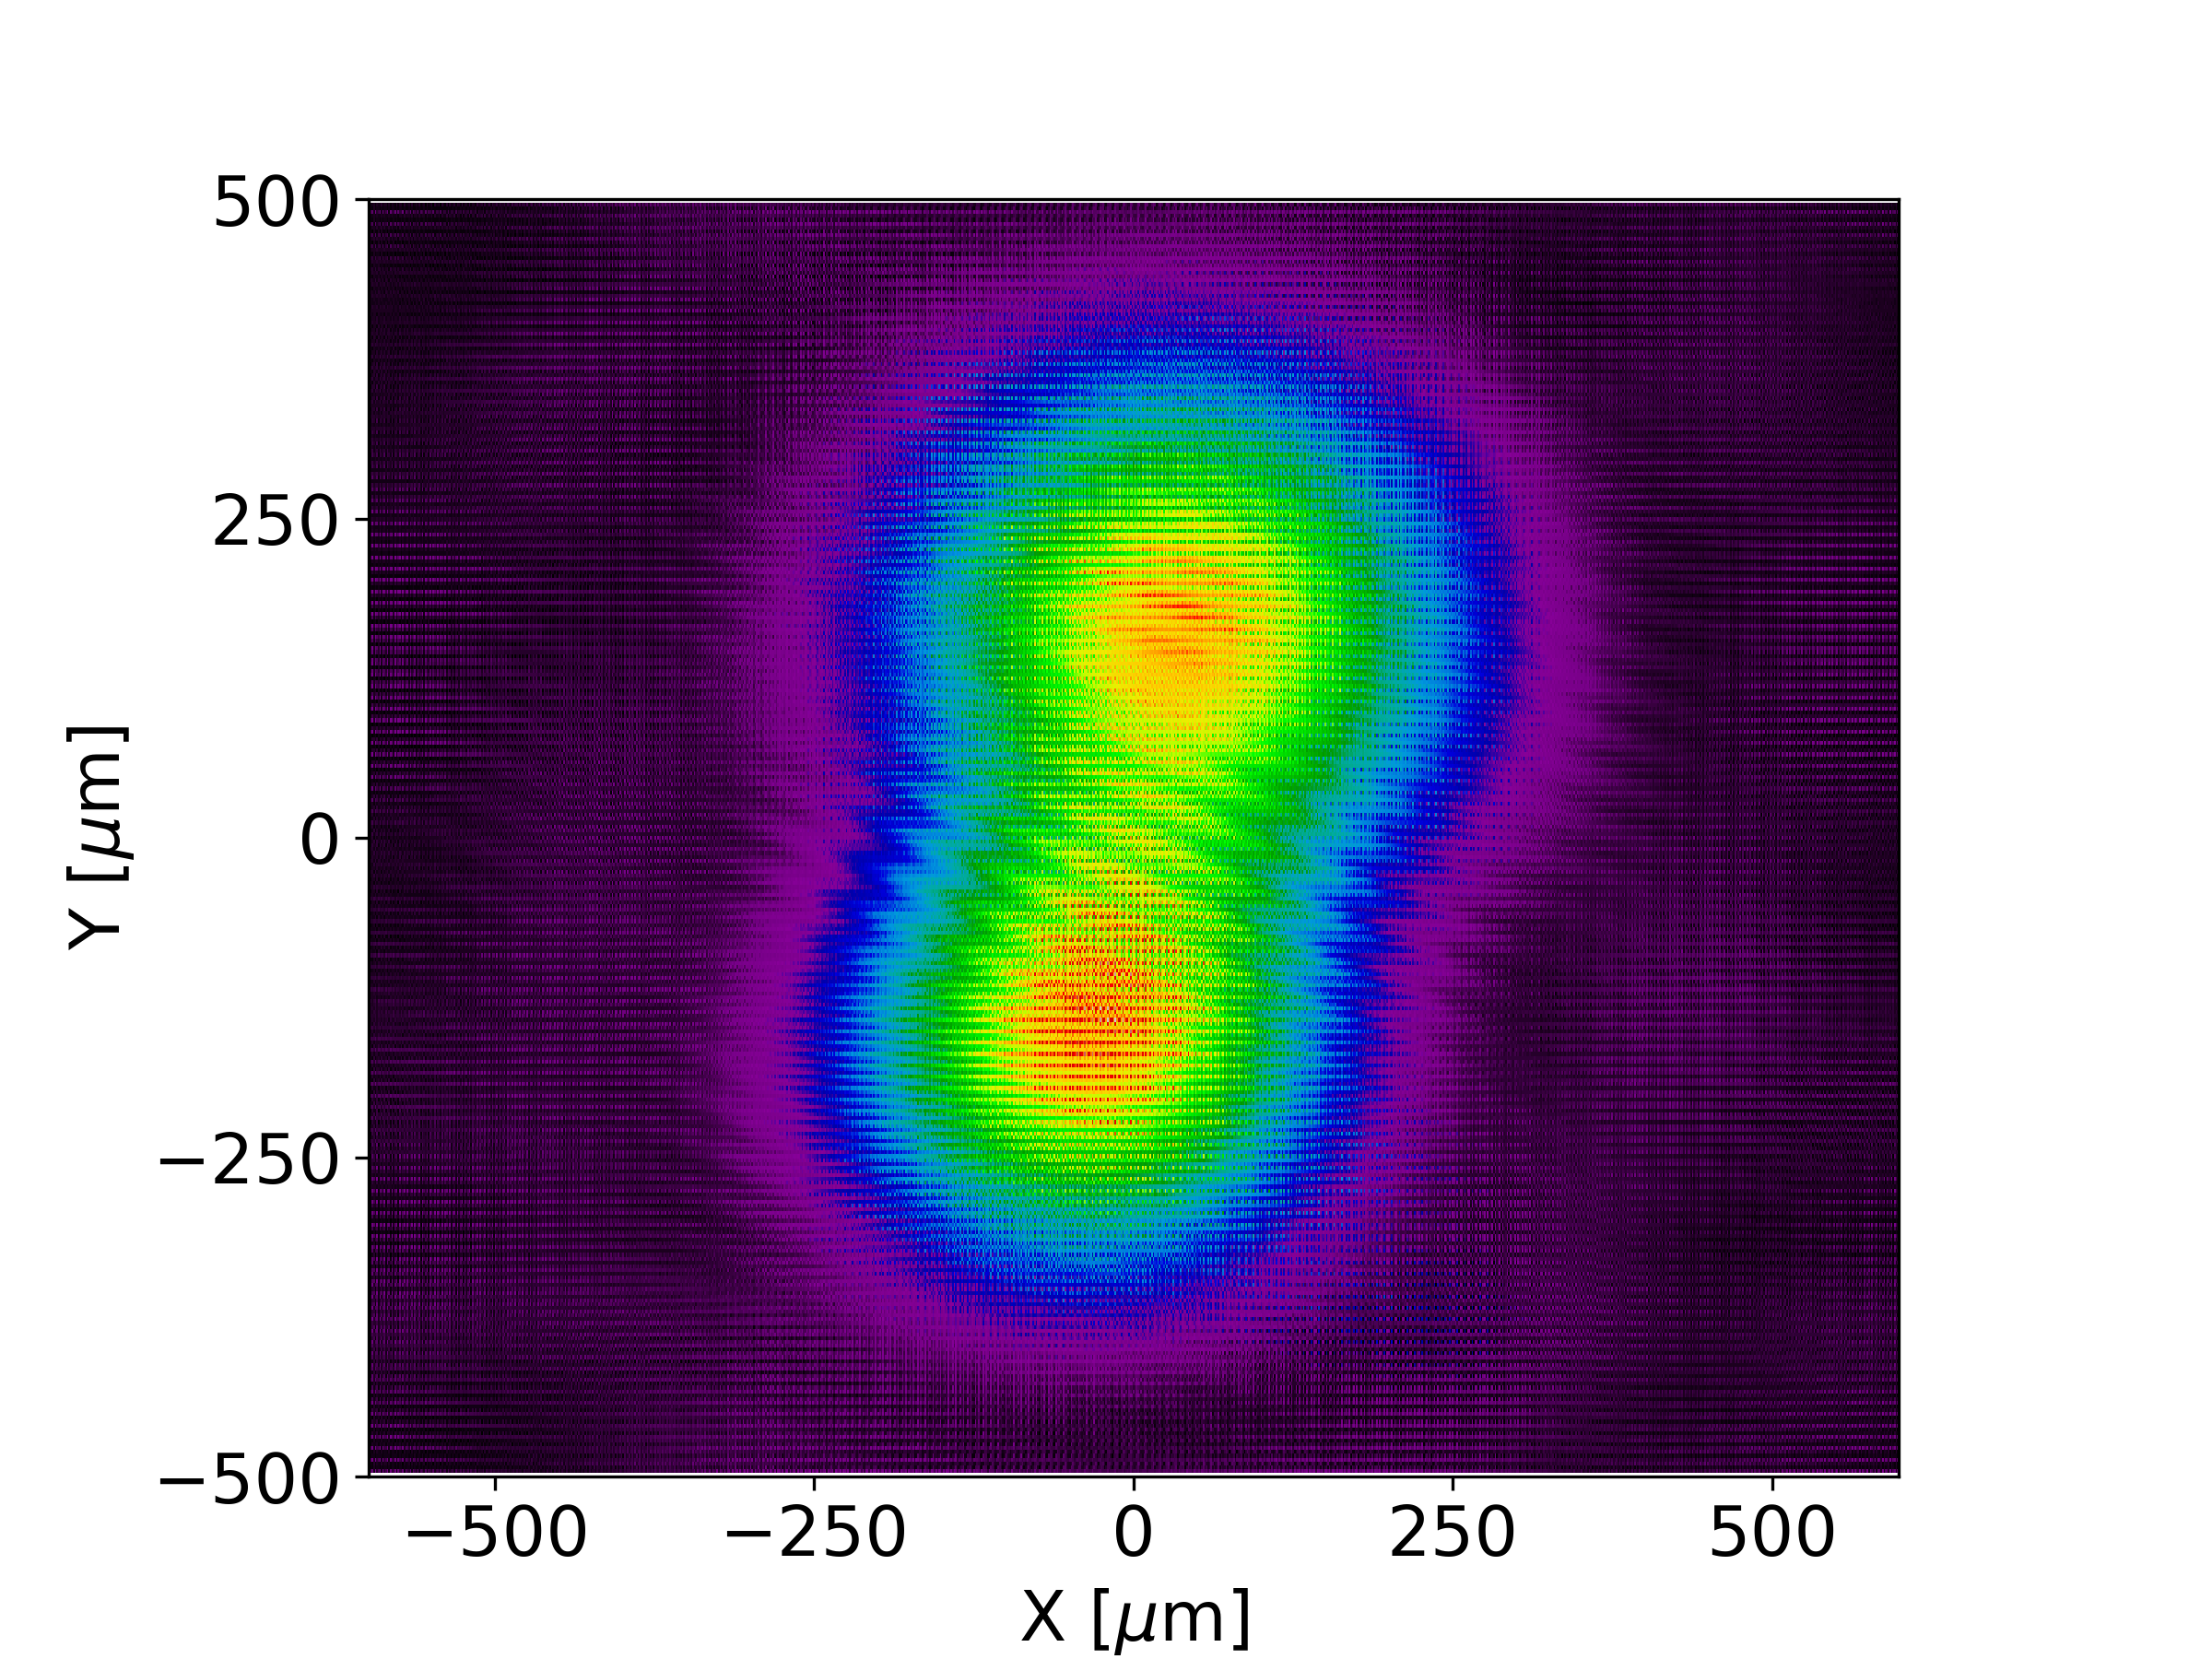
\includegraphics[width=4cm]{Figures/interference_D_uptomode0006_pattern.png}

\label{young}
\end{figure}

%
%%
%%%
%%%
%%
%

\begin{figure}
\caption{The same as Fig.~\ref{young} but using 19,20 and 100 modes for building the CSD.}


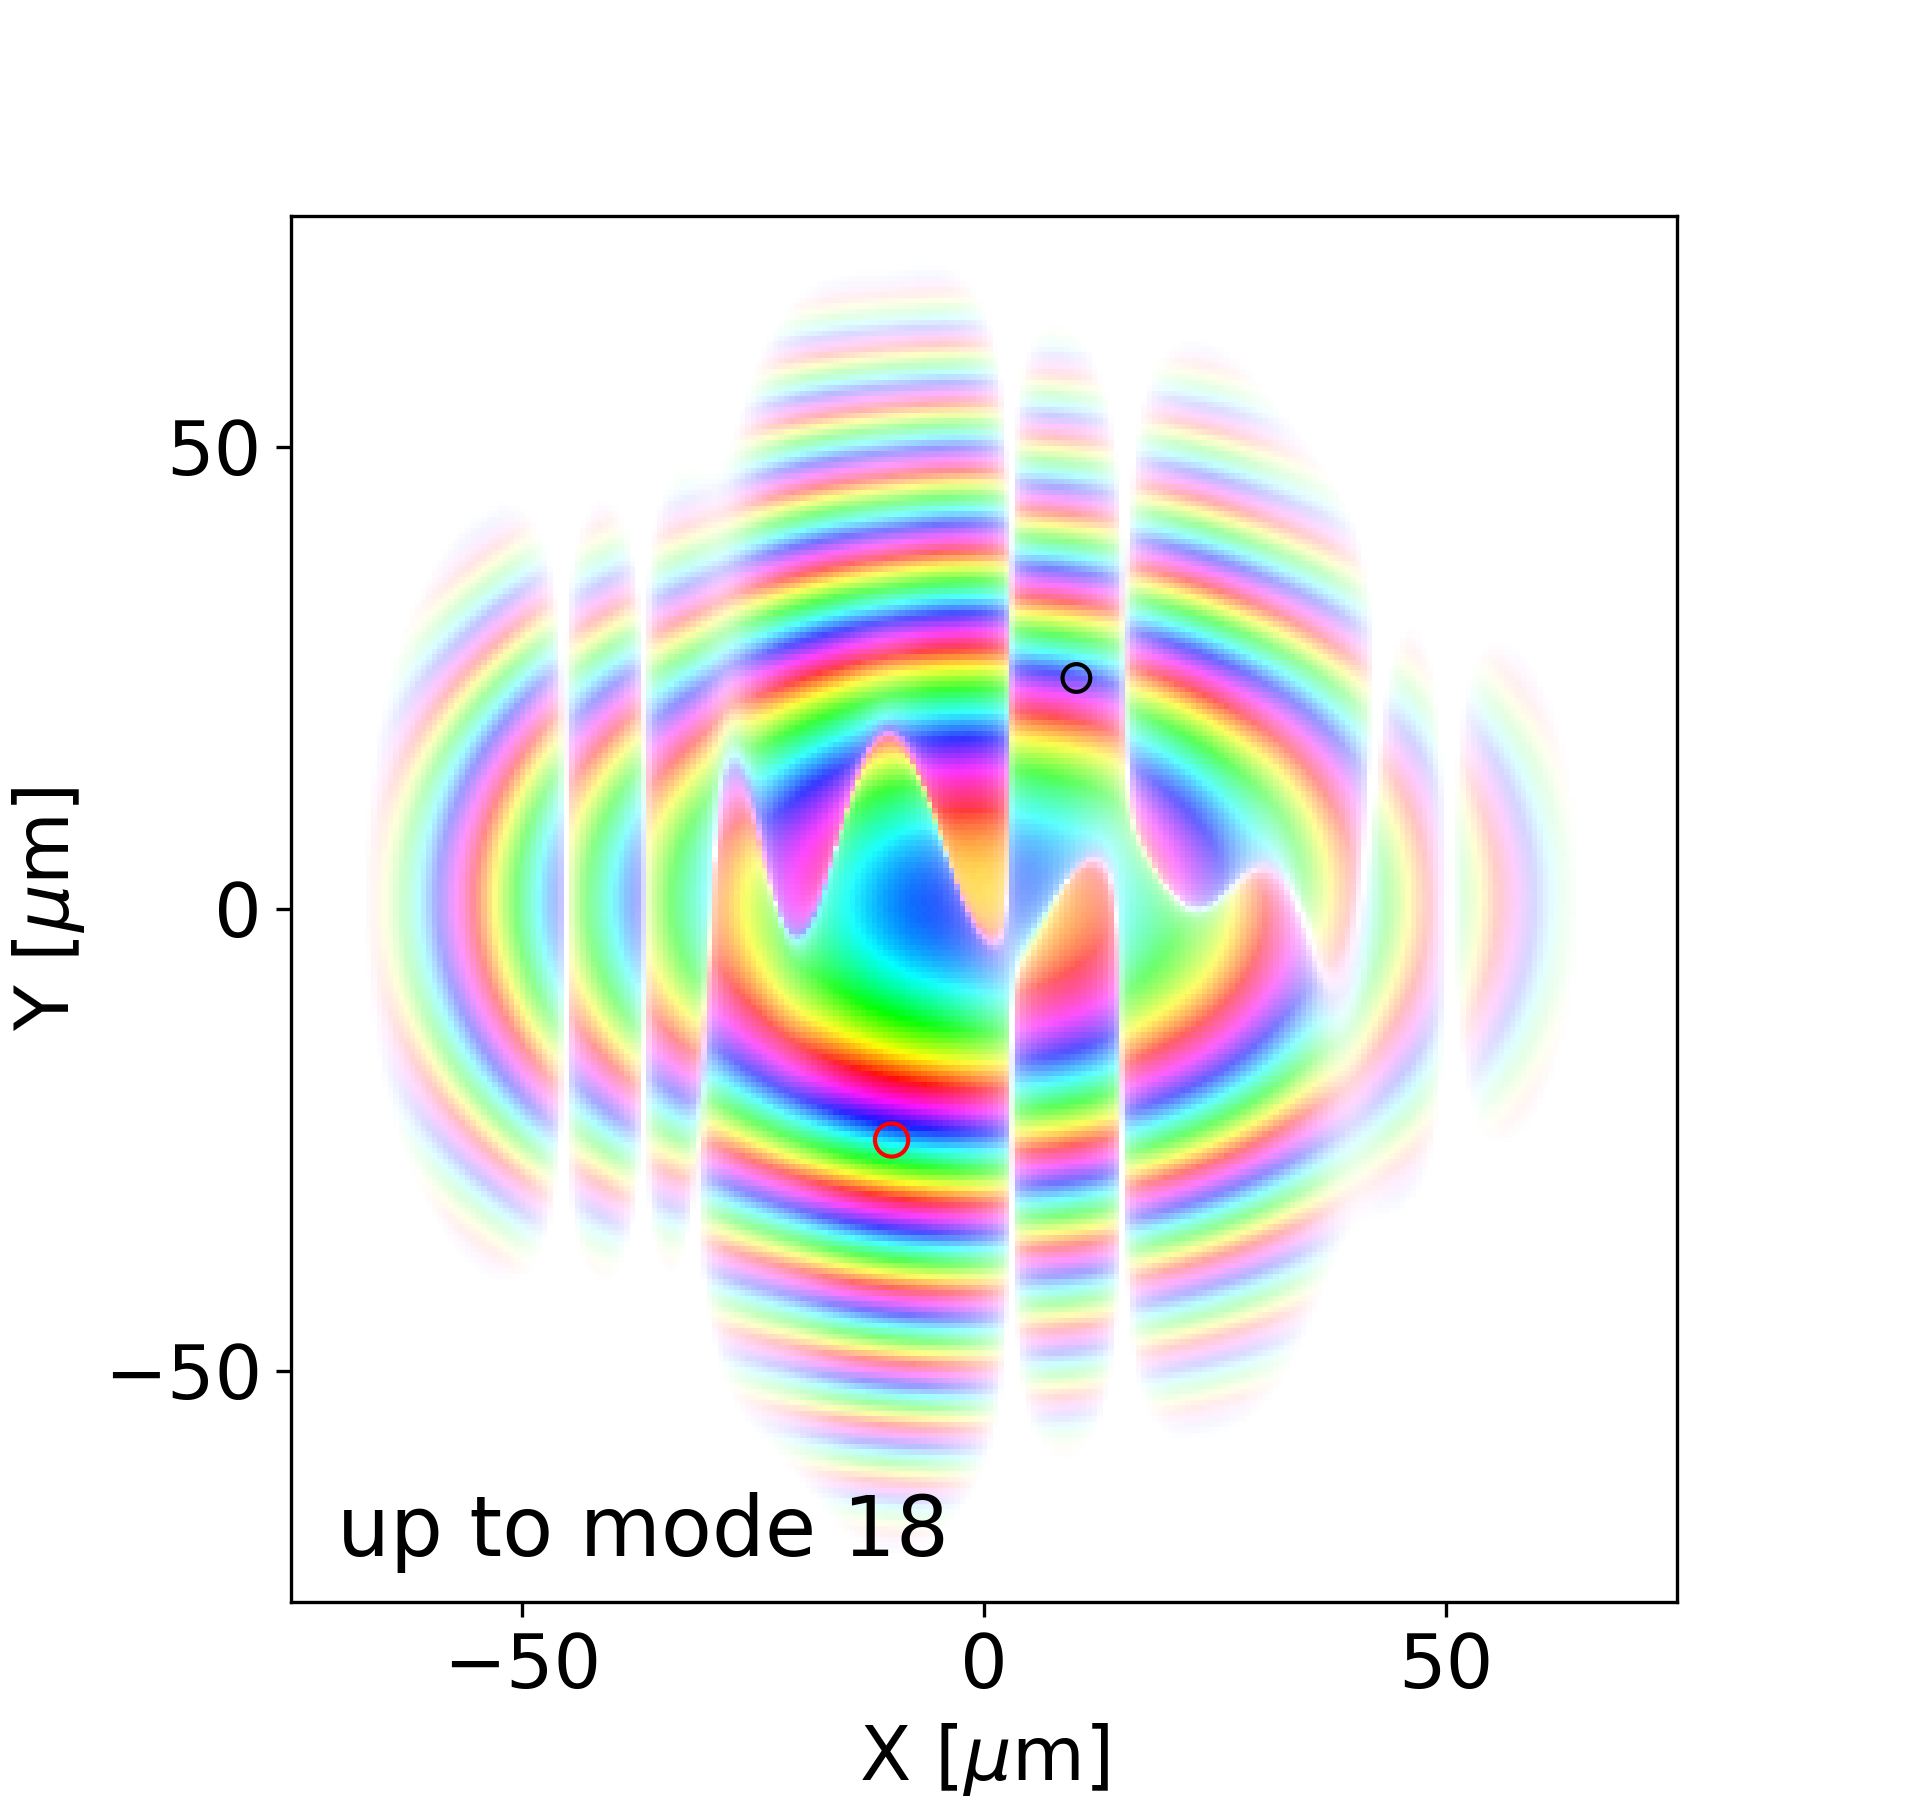
\includegraphics[width=4cm]{Figures/interference_D_uptomode0018_csd.png}
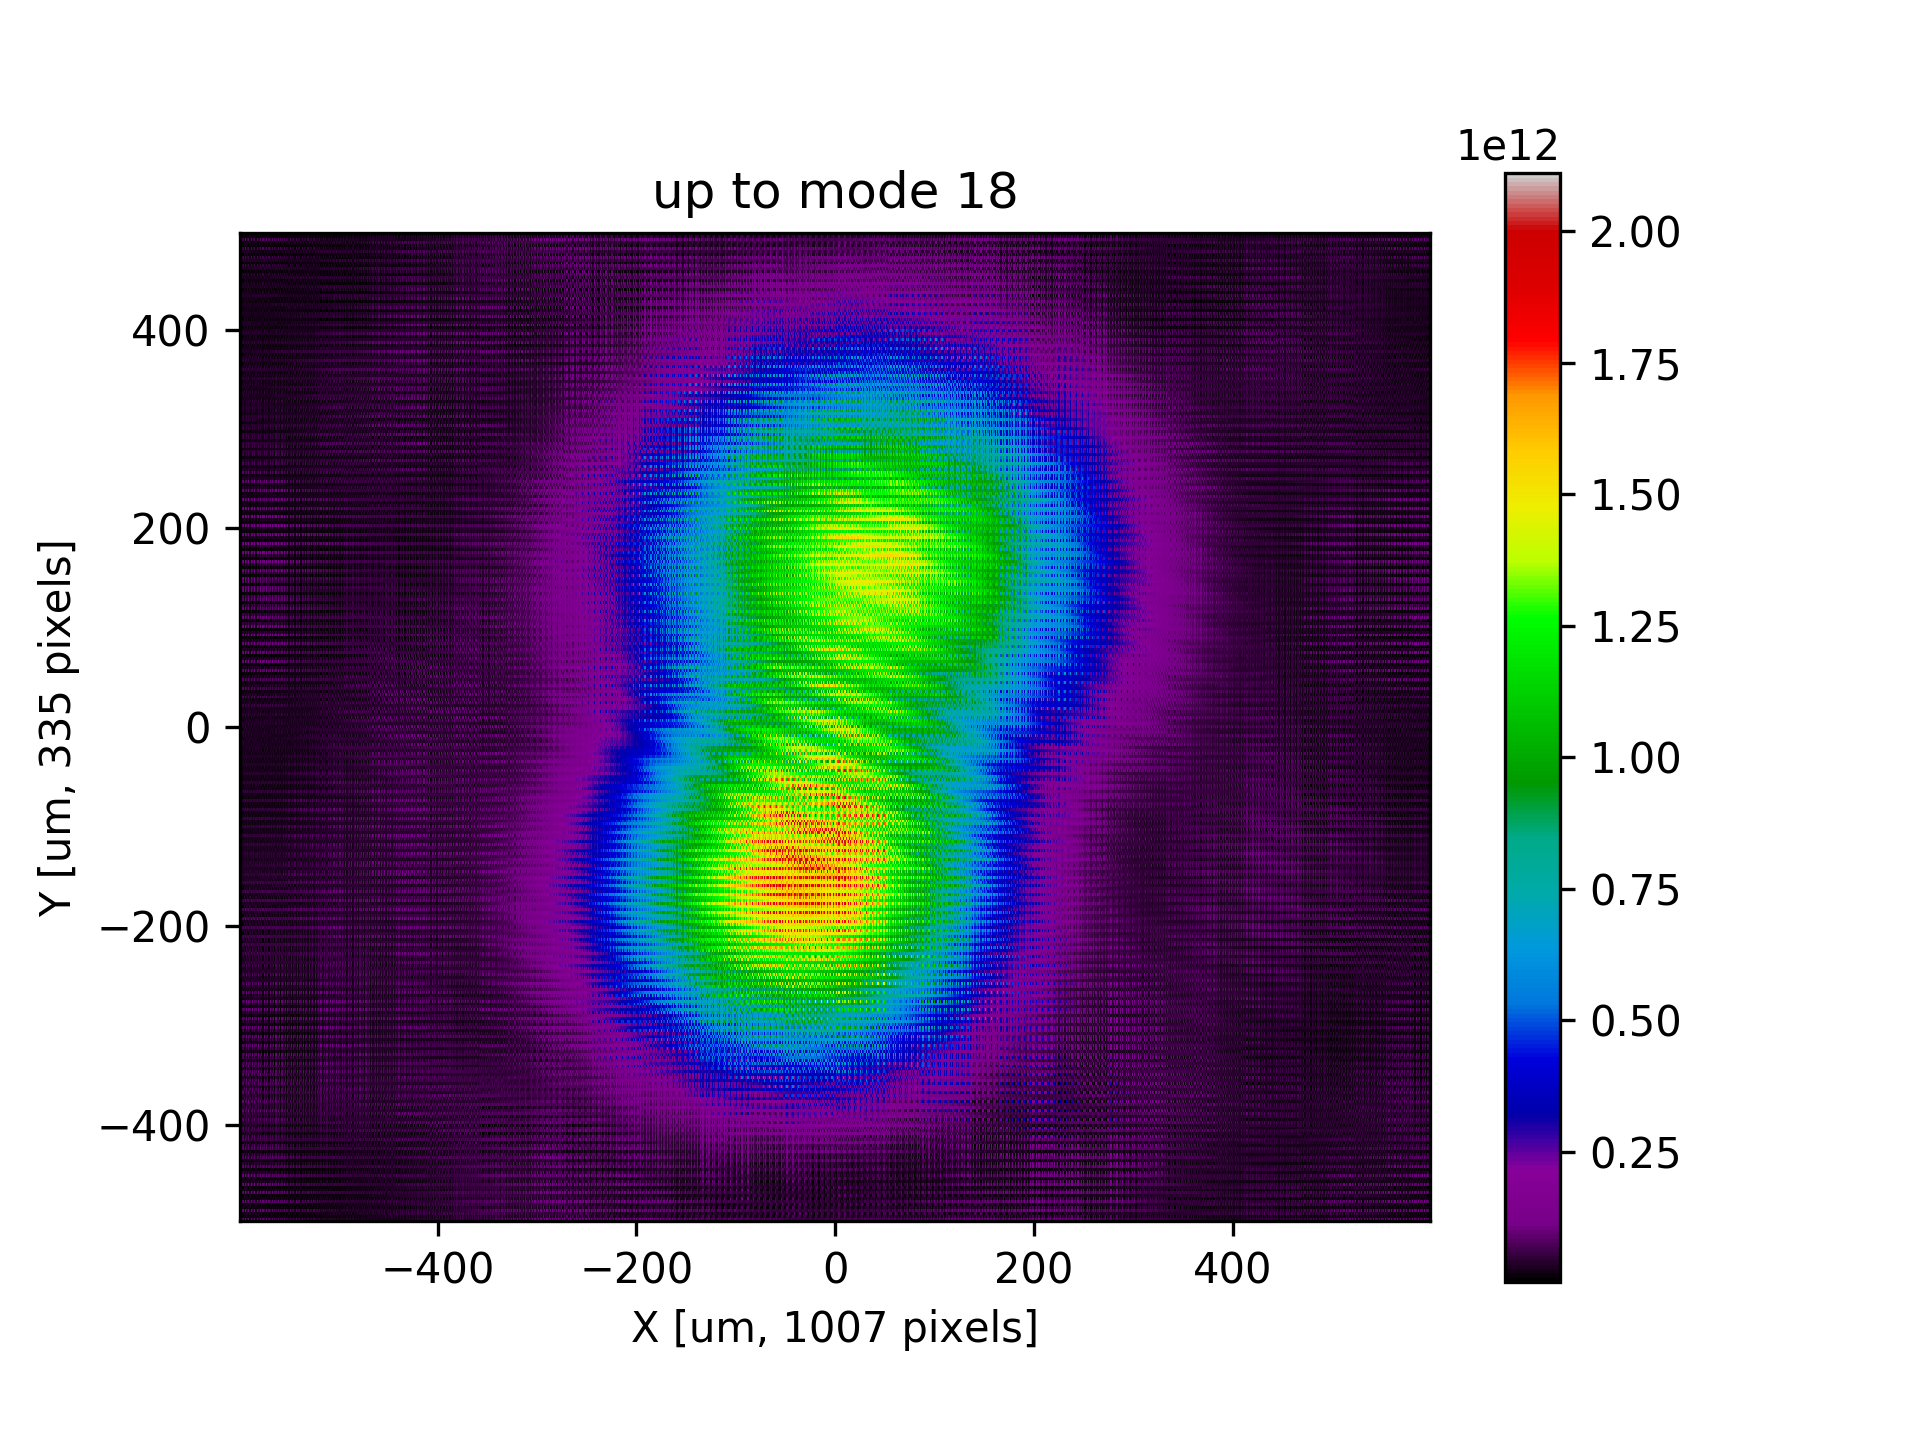
\includegraphics[width=4cm]{Figures/interference_D_uptomode0018_pattern.png}

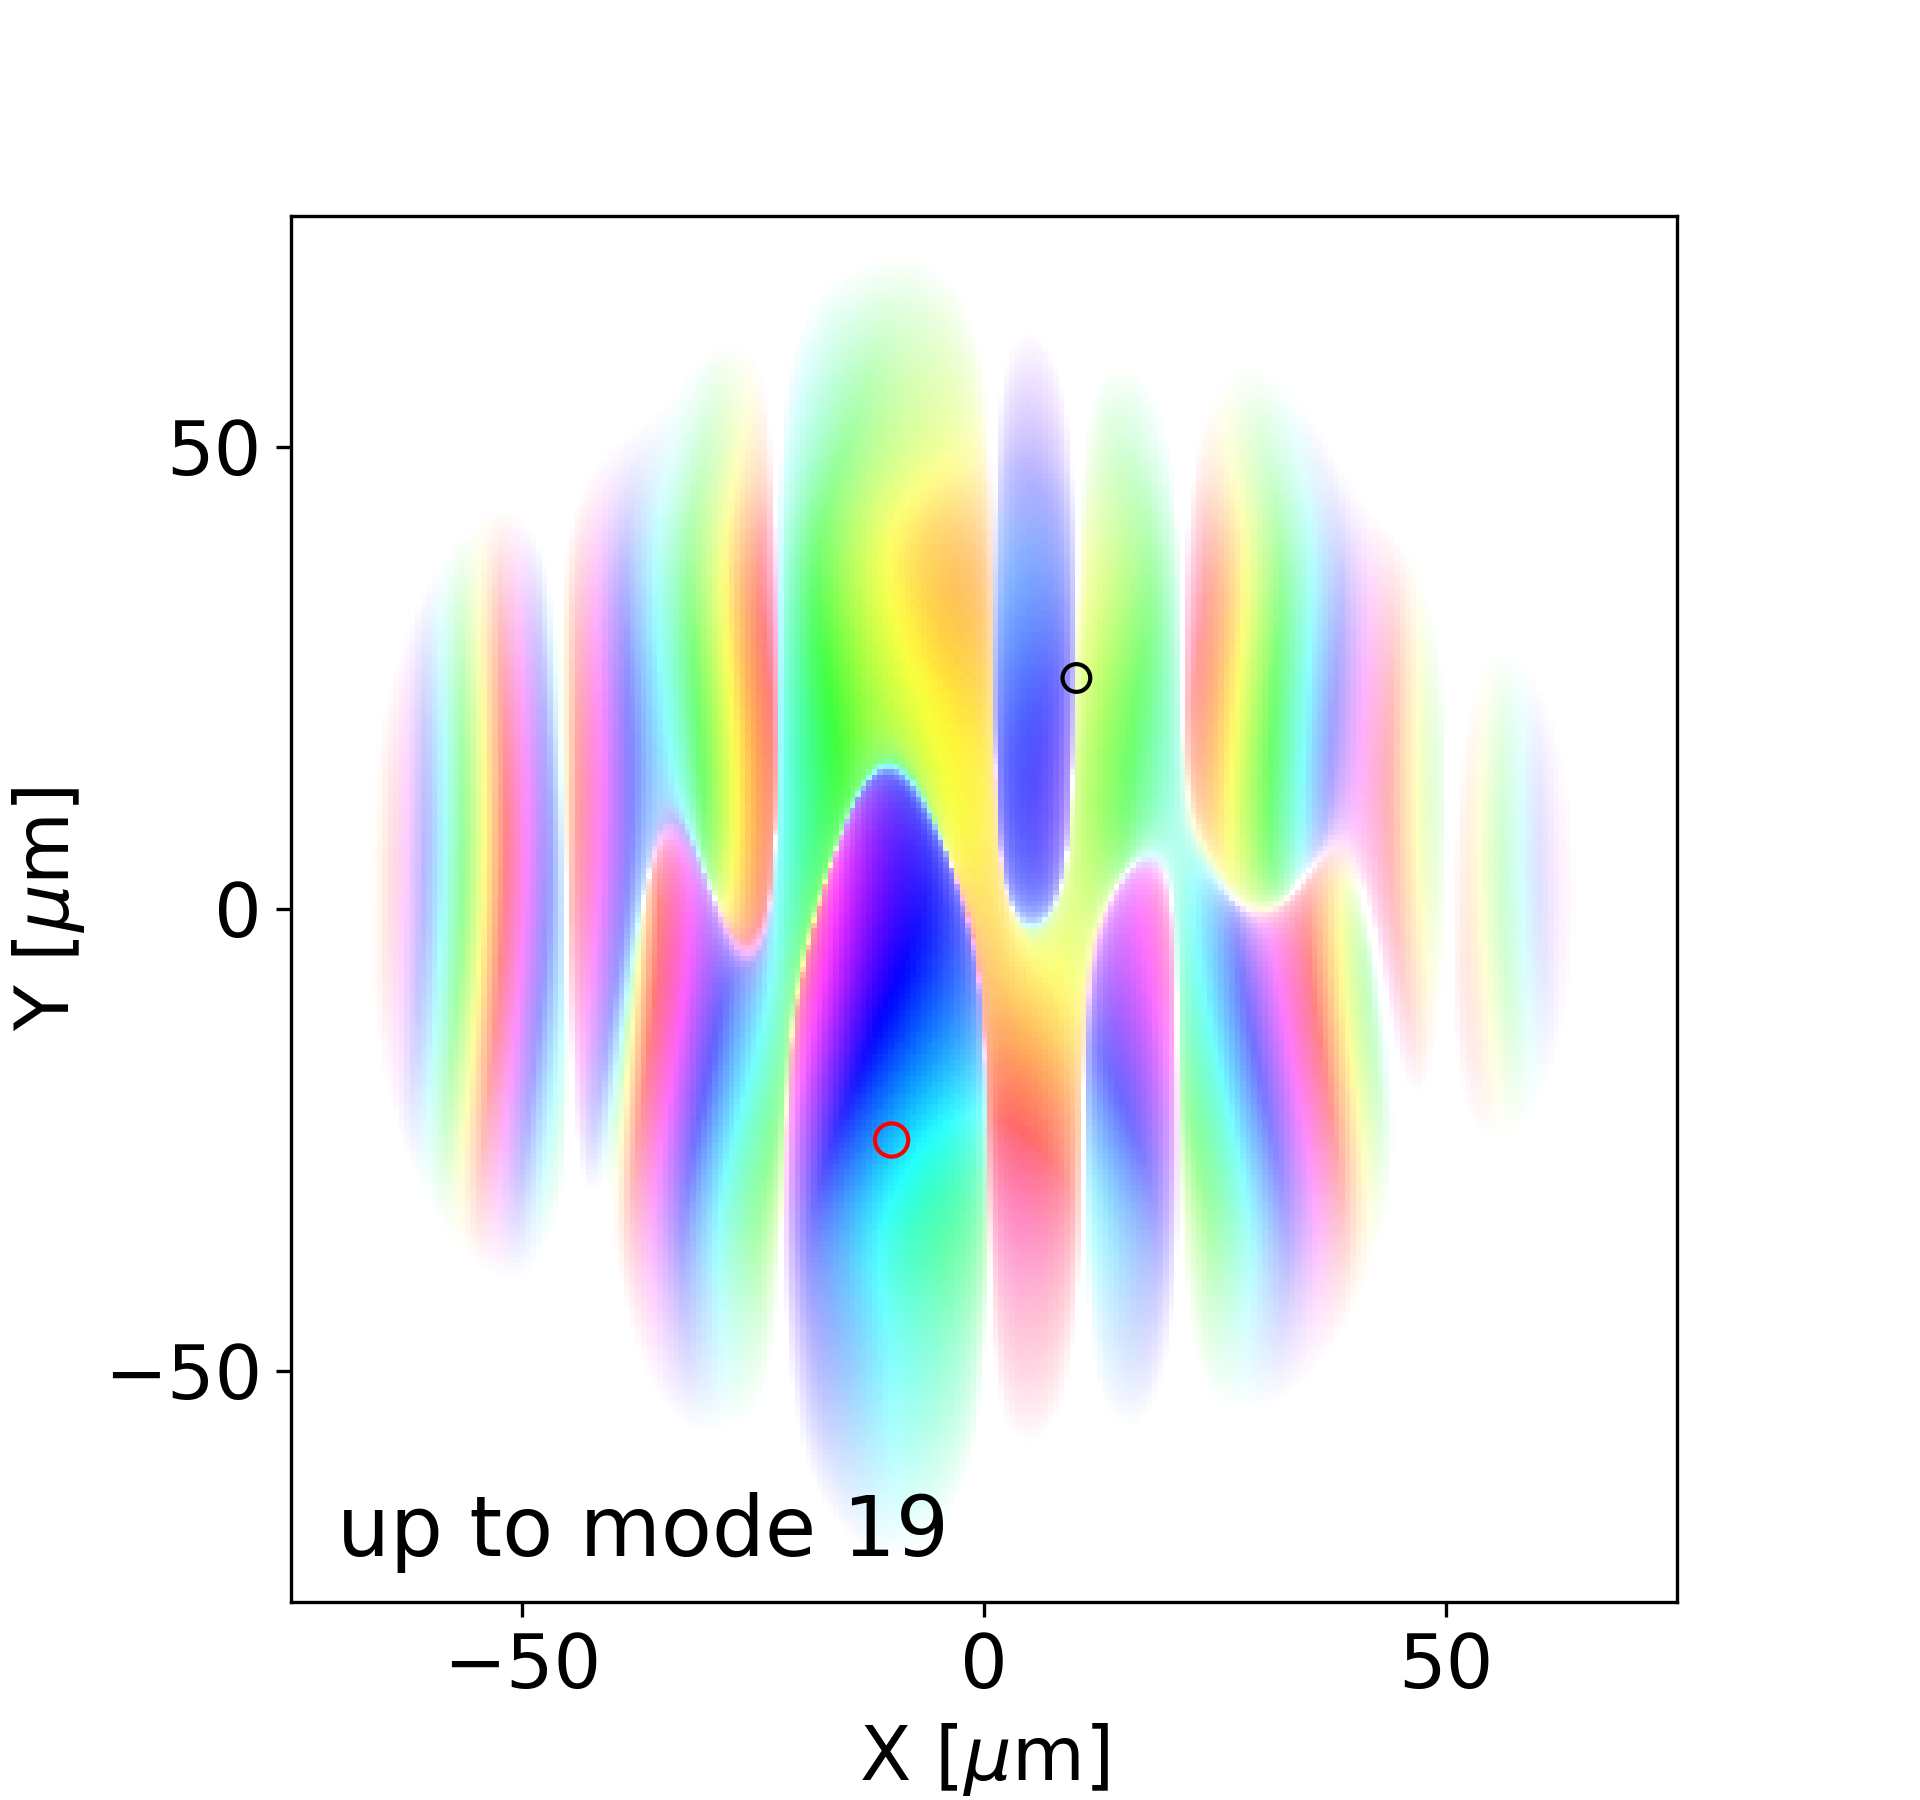
\includegraphics[width=4cm]{Figures/interference_D_uptomode0019_csd.png}
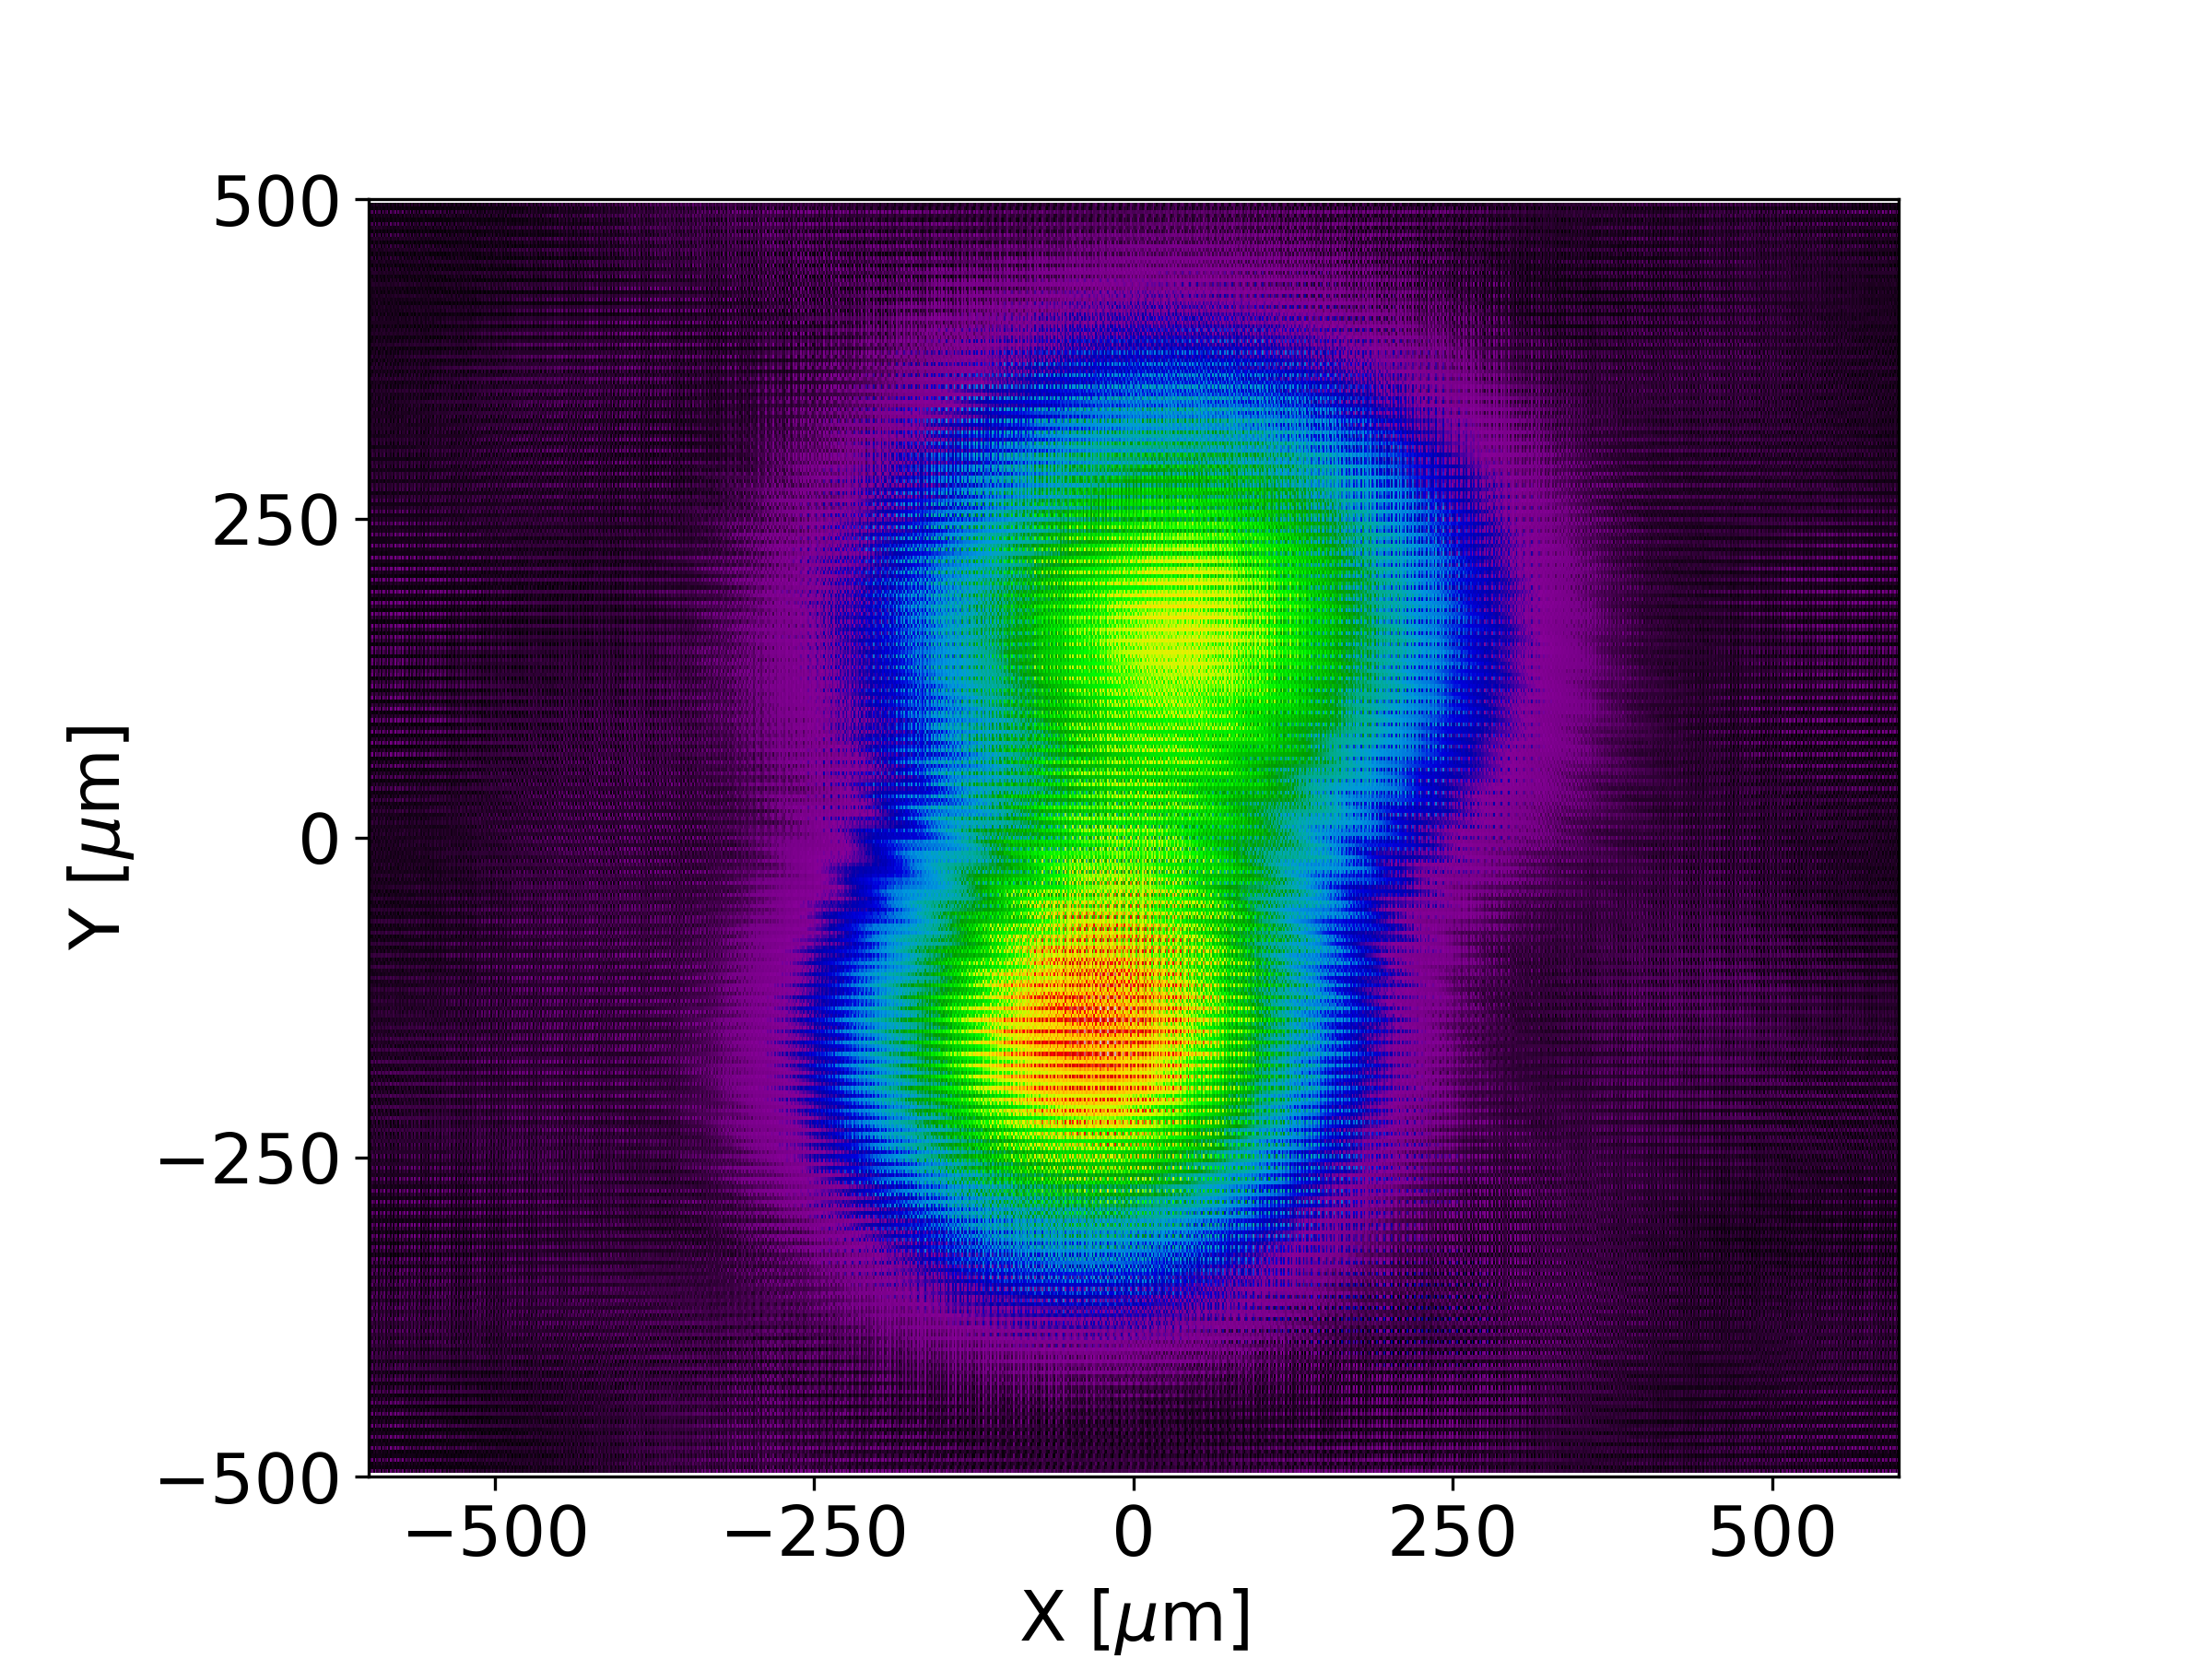
\includegraphics[width=4cm]{Figures/interference_D_uptomode0019_pattern.png}

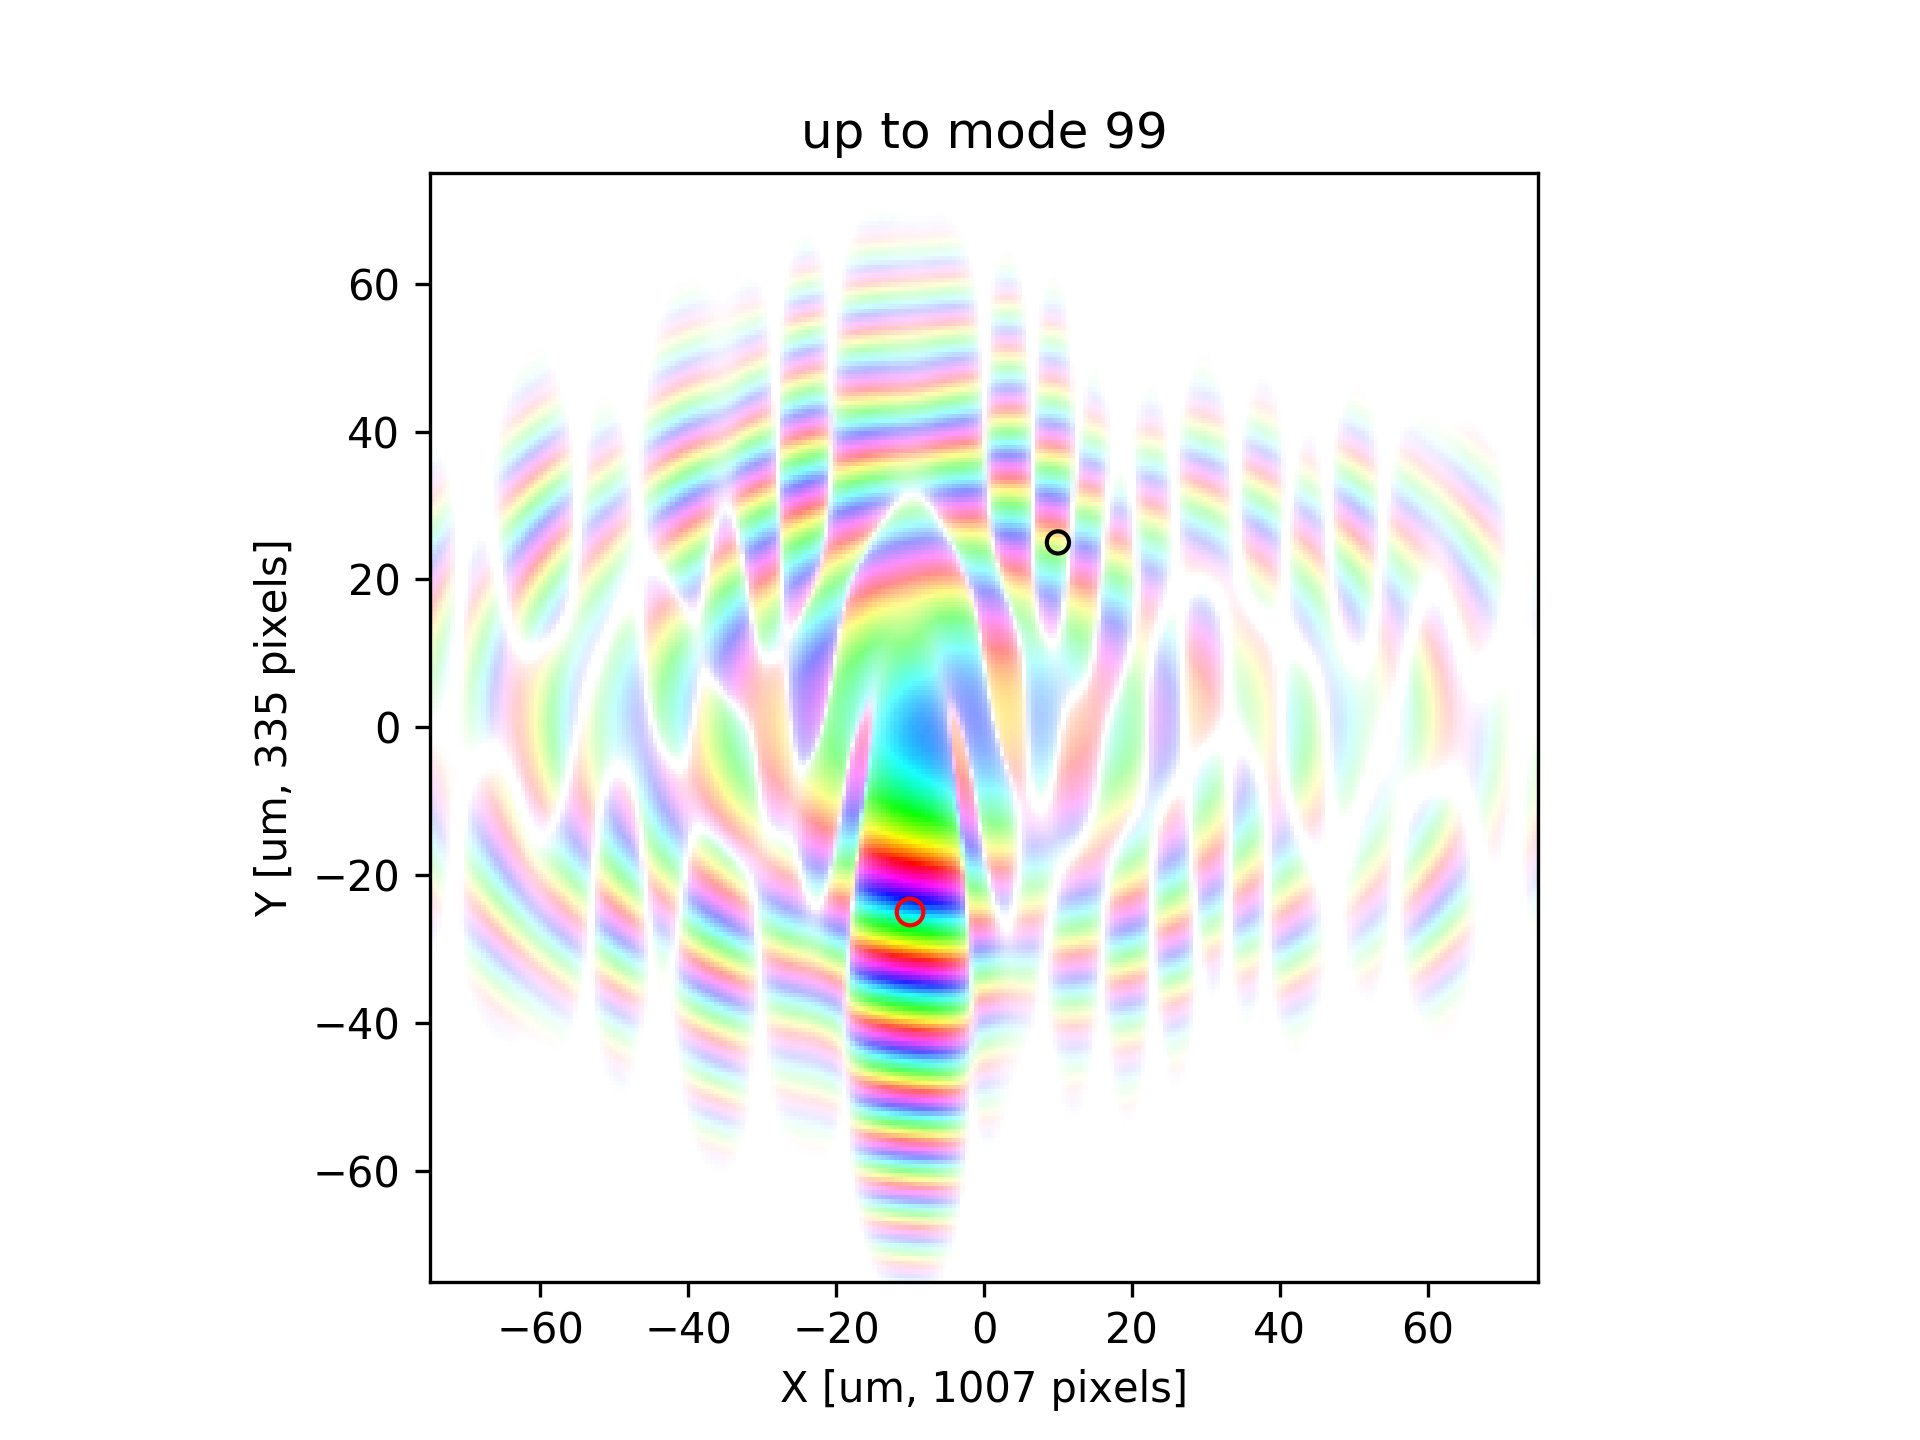
\includegraphics[width=4cm]{Figures/interference_D_uptomode0099_csd.png}
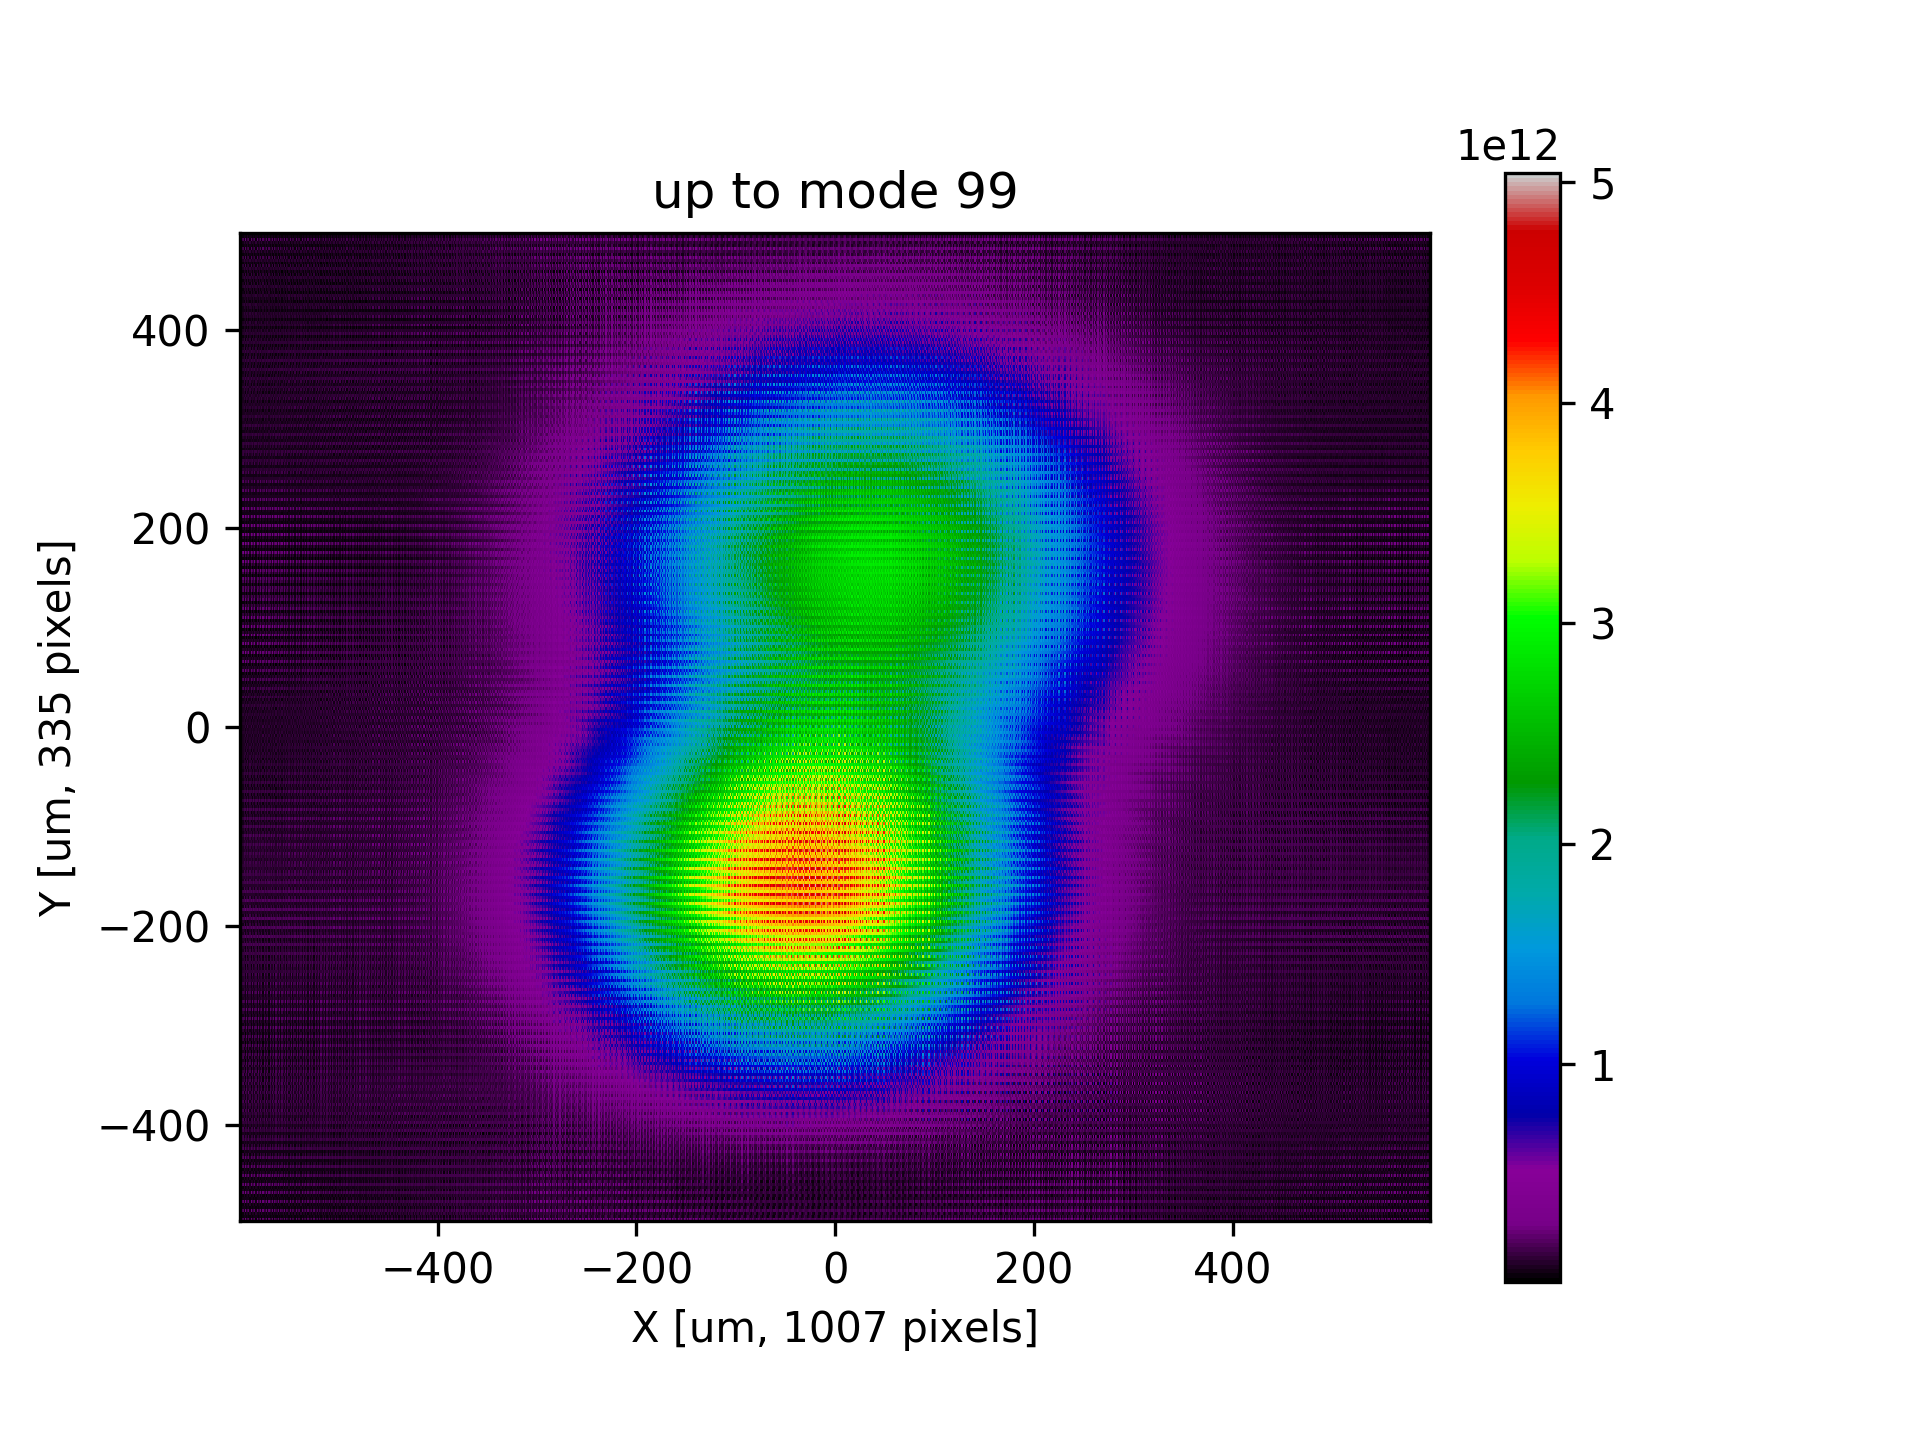
\includegraphics[width=4cm]{Figures/interference_D_uptomode0099_pattern.png}

\label{young2}
\end{figure}


\section{Discussion}

WHEN YOU WORK ON THE REVISIONS, YOU NEED TO TIE THE DISCUSSION A  LITTLE CLOSER TO THE SIMULATIONS THAT HAVE BEEN ADDED SINCE THE DISCUSSION WAS FIRAST DRAFTED.

{\color{red} This needs to be included somewhere in the discussion: Coherence vortices are seen to persist even if the most populated coherent mode has a relatively large fraction of the total optical power, corresponding to a high coherent fraction and a source that has a high degree of coherence.}

This discussion in broken into three sub-sections.  Section~\ref{subsec:Discussion-part-1} considers the influence of CSD correlation singularities, and the closely related phenomenon of CSD speckles, on measured spectral densities.  Section~\ref{subsec:Discussion-part-2} explores the broad connection between unresolved speckle and the formalism of partially coherent light, with particular reference to the role of CSD correlations singularities in this context.  Finally, Section~\ref{subsec:Discussion-part-3} outlines some possible avenues for future work.  

\subsection{Influence of CSD speckle on measured spectral densities}\label{subsec:Discussion-part-1}

The speckled CSDs considered in the present paper will influence on intensity data that are measured in a variety of experiments.  Speaking in very general terms, the measured intensity data for this totality of all possible experiments, will involve a coarse-graining over both the CSD and over the structure of any sample that may be present, together with any optical elements that are introduced after the undulator.  The speckled structure of CSDs such as that considered here will influence measured intensity data in possibly subtle ways, a point we now explore in more detail.  

As a simple example, consider the scattered CSD due to the presence of a scalar non-magnetic scattering potential $F(x,y,z,\omega)$ associated with a static sample having complex refractive index $n(x,y,z,\omega)$ \cite{mandel_wolf}:
\begin{equation}
\begin{aligned}
\label{eq:ScatteringPotential}
F(x,y,z,\omega)=\frac{k^2}{4\pi}[n^2(x,y,z,\omega)-1].
\end{aligned}
\end{equation}
Under the first Born approximation, the scattered CSD resulting from an incident CSD $W^{(i)}$ is \cite{wolf_thin_book}:
\begin{equation}
\begin{aligned}
W^{(s)} ({\bf r}_{\perp 1}, z_1=z, & {\bf r}_{\perp 2},z_2=z) \\ 
=  \int \!\!\! \int \!\!\! \int \!\!\! \int \!\!\! \int \!\!\! \int &  W^{(i)}({\bf r}_{\perp 1}',z_1',{\bf r}_{\perp 2}',z_2',\omega)
\\ &\times F^*({\bf r}_{\perp 1}',z_1',\omega)~F({\bf r}_{\perp 2}',z_2',\omega) \\ &\times G^*({\bf r}_{\perp 1},z_1=z;{\bf r}_{\perp 1}',z'_1=z;\omega) \\ &\times G({\bf r}_{\perp 2},z_2=z;{\bf r}_{\perp 2}',z'_2=z;\omega) \\ &\times d{\bf r}_{\perp 1}'~dz'_1~{\bf r}_{\perp 2}'~dz'_2,
\label{eq:CSDScatteringFirstBornApproximation}
\end{aligned}
\end{equation}
where
\begin{equation}
\begin{aligned}
G( & {\bf r}_{\perp 1},z_1; {\bf r}_{\perp 2},z_2;\omega) \\ &=\frac{\exp[i \omega c^{-1}\sqrt{ | {\bf r}_{\perp 2}-{\bf r}_{\perp 1}|^2+(z_1-z_2)^2}]}{\sqrt{| {\bf r}_{\perp 2}-{\bf r}_{\perp 1}|^2+(z_1-z_2)^2}}
\end{aligned}
\end{equation}
is the outgoing free-space Green function for the Helmholtz equation, and  ${\bf r}_{\perp j}\equiv(x_j,y_j)$ where $j=1,2$.

Consider a sample that consists of a pair of point-like scatterers, whose positions happen to coincide with the locations $A=({\bf r}_{\perp 1}'',z'')$ and $B=({\bf r}_{\perp 2}'',z'')$ associated with a coherence-vortex core. This amounts to Fig.~\ref{loss_of_fringe_visibility}(a), with the screen removed and the pinholes at $A$ and $B$ being replaced with small scatterers at the same locations.  The associated scattering potential is:
\begin{equation}
\begin{aligned}
F({\bf r}_{\perp},z,\omega) &= \mathcal{A}(\omega)~ \delta({\bf r}_{\perp}-{\bf r}_{\perp 1}'',z-z'',\omega) \\ &+ \mathcal{B}(\omega) ~\delta({\bf r}_{\perp}-{\bf r}_{\perp 2}'',z-z'',\omega),
\label{eq:ScatteringPotentialTwoDots}
\end{aligned}
\end{equation}
where the scattering amplitudes $\mathcal{A}$ and $\mathcal{B}$ are complex functions of energy $\hbar\omega$, and $\delta$ is a Dirac delta in three-dimensional space.   Since $W^{(i)}({\bf r}_{\perp 1}'',z'',{\bf r}_{\perp 2}'',z'',\omega)$ vanishes on account of the coherence vortex, and the Hermitian character of the CSD \cite{mandel_wolf} implies that $W^{(i)}({\bf r}_{\perp 2}'',z'',{\bf r}_{\perp 1}'',z'',\omega)$ also vanishes, substitution of Eq.~\ref{eq:ScatteringPotentialTwoDots} into Eq.~\ref{eq:CSDScatteringFirstBornApproximation} leads to:
\begin{equation}
\begin{aligned}
\label{eq:CSDsforTwoScattersAtCVCore}
W^{(s)} ({\bf r}_{\perp 1}, &z_1=z, {\bf r}_{\perp 2},z_2=z) \\ = ~ &W^{(s)}_A ({\bf r}_{\perp 1}, z_1=z,  {\bf r}_{\perp 2},z_2=z) \\ &+ W^{(s)}_B ({\bf r}_{\perp 1}, z_1=z, {\bf r}_{\perp 2},z_2=z).
\end{aligned}
\end{equation}
Here, $W^{(s)}_A ({\bf r}_{\perp 1}, z_1=z, {\bf r}_{\perp 2},z_2=z)$ is the scattered CSD that would have been obtained if the scatterer at $A$ were to be present but the scatterer at $B$ were to be removed, with $W^{(s)}_B ({\bf r}_{\perp 1}, z_1=z, {\bf r}_{\perp 2},z_2=z)$ being the scattered CSD that would have been obtained if the scatterer at $B$ were to be present but the scatterer at $A$ were to be removed.  
\todo{MSR: This addition of $W$ is interesting and could be checked numerically. In Fig~\ref{young} I propagated $W$ five meters to a plane where I put the apertures D and E. I apply the apertures to all modes to I have $W_{D,E}$ that I propagate 30m to the image plane where I calculate the Spectral Density $W_{DE}^{prop}(x,y,x,y)$. As theory suggest $W_{E,F}^{prop}=W_{E}^{prop}+W_{F}^{prop}$ so we can compare for instance the phase of $W$. The problem is that the apertures of slits are not additionable. Solid stoppers would be additionable, but a slit acts a a ``negative'' object, just absorbing everything out of it. To be discussed by skype!!.}
Upon setting ${\bf r}_{\perp 1}={\bf r}_{\perp 2}$ to convert the CSD into the spectral density, we see that the spectral densities scattered from $A$ and $B$ respectively, merely add incoherently, with the usual interference term that would otherwise be present in the spectral interference law \cite{mandel_wolf} being suppressed by the coherence vortex.  Thus, if the pair of scatterers at $A$ and $B$, the scattering from which produces no interference fringes, were to be rigidly transversely displaced or rotated in the beam, such that the pair of scatterers no longer coincided with a coherence vortex, the interference term in the spectral interference law would cease to be suppressed and Young-type fringes would appear on account of the superposing of the now-partially-correlated radiation emanating from each of the scatterers.  The concept of a transverse coherence length, which is meaningful in both a conceptual and a computational sense when the pair of scatterers do not coincide with a pair of transverse coordinates associated with a coherence vortex, ceases to be meaningful (and generates the incorrect expectation of Young-type fringes associated with partially correlated disturbances emanating from the pair of scatterers) when the pair of scatterers coincides with a coherence vortex.     

The above conclusion is illustrated in Fig.~\ref{fig:ABCD}.  Here, as before, the pair of points $A$ and $B$ correspond to a coherence-vortex core, when both of these points lie in the plane $\alpha$. The locations $C$ and $D$ in the plane $\alpha$, do not correspond to a coherence vortex.  When a point scatterer is placed at $A$ and $C$ in the plane $\alpha$, for example, and the resulting cross-spectral density propagated to the downstream plane $\beta$ and thence used to compute the measured spectral density, Fig.~\ref{fig:ABCD}(a) results.  Here, Young-type interference fringes are formed, with a non-maximal visibility on account of the fact that the radiation is partially coherent.  If the pair of scatterers is instead located at $A$ and $B$, corresponding to a coherence vortex core, the associated fringe visibility drops to zero---see Fig.~\ref{fig:ABCD}(b).  If one were to have three scatterers, say at $A$ and $B$ and $C$ in the plane $\alpha$, then one would would observe a spectral density such as that shown in Fig.~\ref{fig:ABCD}(c), with interference fringes being present due to the overlap of radiation scattered from $A$ and $C$, and also from $B$ and $C$, but with no fringes resulting from the superposition of the radiation scattered from $A$ and $B$.    No such fringe-suppression occurs in Fig.~\ref{fig:ABCD}(d), when the three scatterers are placed at $B,C$ and $D$. 

\begin{figure}
\caption{Example of the influence of a coherence vortex, corresponding to points $A$ and $B$ in the plane $\alpha$, on spectral densities measured over the downstream plane $\beta$.  Of the points $A,B,C,D$ that are indicated, only the pairing $A,B$ coincides with a coherence vortex.  Shown are the spectral densities over the plane $\beta$ that result when scattering centres are placed at (a) $A,C$; (b) $A,B$; (c) $A,B,C$; (d) $B,C,D$.}
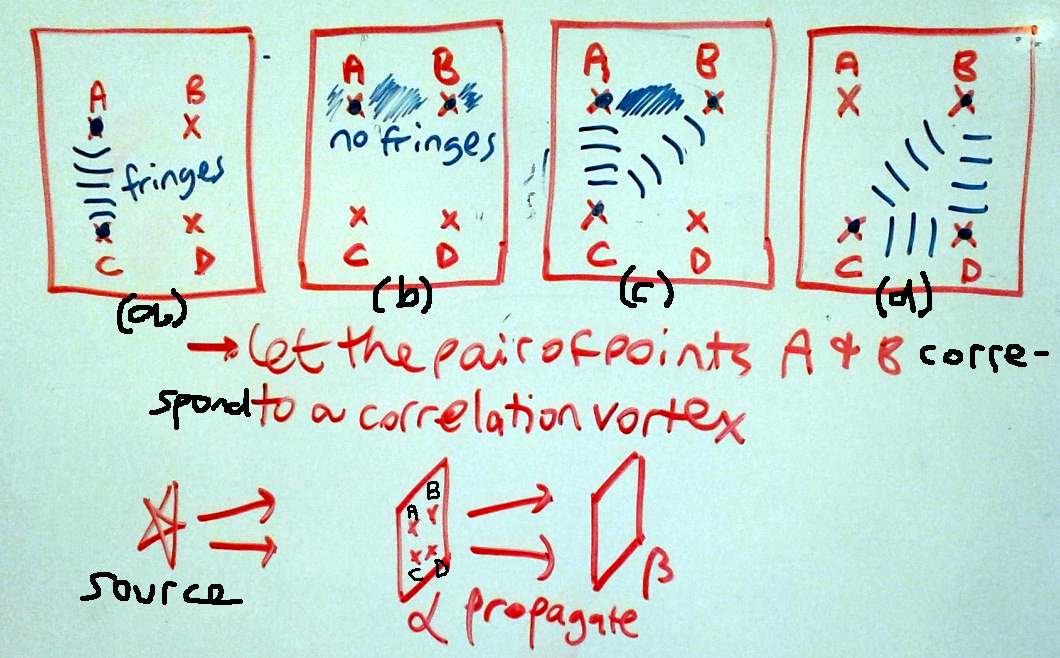
\includegraphics[width=8.5cm]{Figures/ABCD.png}
\label{fig:ABCD}
\end{figure}

As a related but more realistic example of the  influence that coherence vortices can have on measured x-ray spectral densities, consider the scenario shown in Fig.~\ref{fig:ImagingWithCoherenceVortex}.  Here, we have replaced the previously-considered pair of point scatterers, referred to above, with an arbitrary assemblage of scatterers ({\em i.e.} an ``object''), and supplanted the first Born approximation with the projection approximation \cite{paganin_book}.  The thin object, with complex transmission function $T({\bf r}_{\perp},\omega)$ is assumed to lie immediately upstream of the plane $z=Z$, with an object-to-detector distance $\Delta > 0$.  Use the coherent-mode expansion to write down the CSD in the plane $z=Z^-$ immediately upstream of the object, then apply the projection approximation to multiply each of the (paraxial) coherent modes by the complex transmission function of the object.  Next, use the Rayleigh-Sommerfeld diffraction integrals of the first kind \cite{Rayleigh, Sommerfeld, mandel_wolf} to propagate each coherent mode from the nominally planar exit surface $z=Z^+$ of the object to the detector plane at $z=Z+\Delta$.  This leads to the following CSD for pairs of points on the detector surface:     
\begin{equation}
\begin{aligned}
\label{eq:CSD_with_object_and_detector}
W ({\bf r}_{\perp 1}, {\bf r}_{\perp 2},z_1 &=z_2=Z+\Delta,\omega) \\ =\sum_m \lambda_m({\omega}) & \left\{ [\phi_m^*({\bf r}_{\perp 1},\omega)~T^*({\bf r}_{\perp 1},\omega)]\star_1 K({\bf r}_{\perp 1},\Delta,\omega)\right\} \\ \times & \left\{ [\phi_m({\bf r}_{\perp 2},\omega)~T({\bf r}_{\perp 2},\omega)]\star_2 K({\bf r}_{\perp 2},\Delta,\omega)\right\},
\end{aligned}
\end{equation}
where 
\begin{equation}
K=-\frac{1}{2\pi} \frac{\partial}{\partial z} G({\bf r}_{\perp},z,{\bf 0}_{\perp},0;\omega) 
\end{equation}
is the Rayleigh-Sommerfeld convolution kernel, ${\bf 0}_{\perp}\equiv (0,0)$ and $\star_{1,2}$ denotes convolution with respect to ${\bf r}_{\perp 1}$ and ${\bf r}_{\perp 2}$ respectively.  Maps of the corresponding spectral density, obtained by setting ${\bf r}_{\perp 1}={\bf r}_{\perp 2}\equiv{\bf r}_{\perp 1}$ in the CSD, may be viewed as interferograms or inline holograms that are generated by a many point scatterers.   

\begin{figure}
\caption{A statistically stationary X-ray source $S$ generates a paraxial CSD illuminating the nominally planar entrance surface $z=Z^-$ of a thin object $O$.  The exit surface of the object is denoted by $z=Z^+$, with the CSD propagating from this exit surface through a free-space distance $\Delta$, to the surface $z=Z+\Delta$ of a position-sensitive detector.}
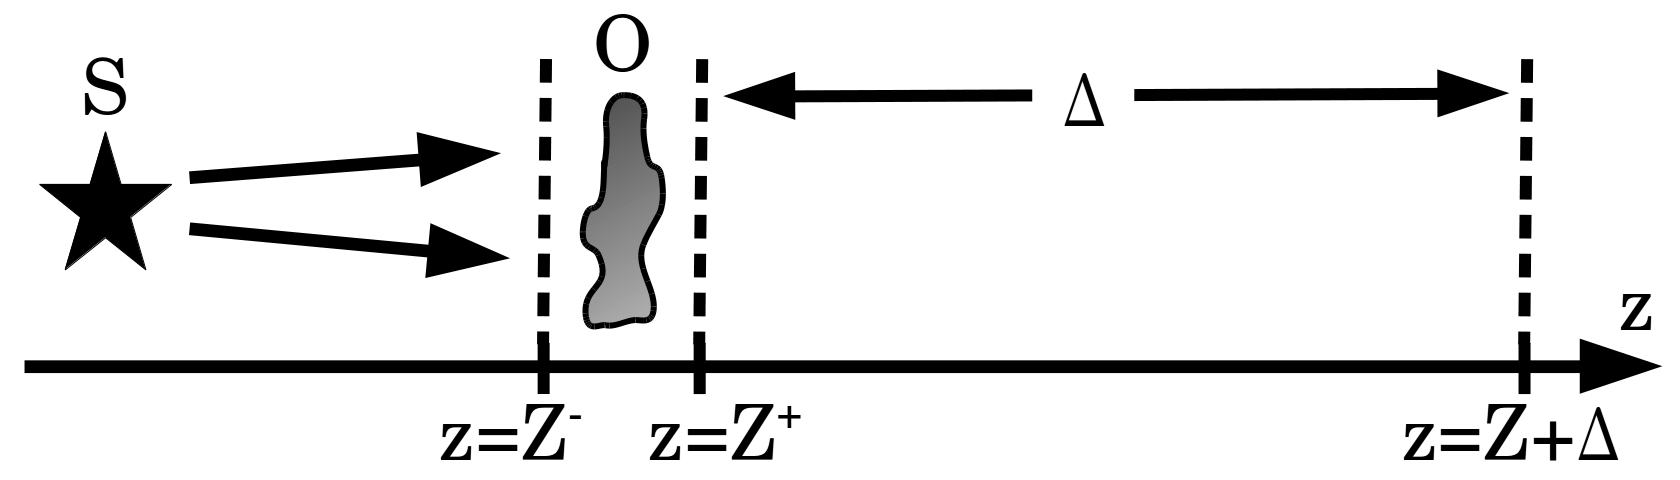
\includegraphics[width=8.5cm]{Figures/ImagingWithCoherenceVortex.png}
\label{fig:ImagingWithCoherenceVortex}
\end{figure}

Whether one considers a pair of point scatterers under the first Born approximation as described by Eqs.~\ref{eq:ScatteringPotential}-\ref{eq:CSDsforTwoScattersAtCVCore}, or a thin object (continuously infinite set of many point scatterers) under the projection approximation as described by Eq.~\ref{eq:CSD_with_object_and_detector}, a similar conclusion is reached regarding the influence of coherence vortices (and the closely related speckle structure in the CSD) on measured spectral densities.  That is, pairs of points in the scattering sample, which happen to coincide with a coherence vortex, will yield a pair of uncorrelated scattered disturbances for which no interference fringes will be formed.  Thus the presence of coherence vortices will influence measured spectral densities, in an effect that in our view warrants further consideration by the x-ray imaging community.  

This is indicative of two broader points that form a key motivation for the present paper: (i) Coherence vortices will exist in most non-trivial x-ray fields, and as such an understanding of their existence will deepen our understanding of imaging and diffraction data obtained using such fields. (ii) Such coherence vortices influence the images that one takes, in ways that may lead to misleading results if one simply ignores their existence.   

\subsection{On the role of unresolved speckle in partial coherence}\label{subsec:Discussion-part-2}

Unresolved speckle lies at the heart of many phenomena exhibited by partially coherent classical optical fields in general, and classical x-ray fields in particular \cite{Nugent2003,paganin_book,Nesterets2008}.  Here, speckles are considered to be unresolved if they are coarse grained over space (via the spatial extent of a detector pixel) or coarse-grained over time (via the acquisition time during which photons are detected).  Note also that ``speckle'' is here used in a broad sense to functions that exhibit rapid variation with respect to spatial variables, a definition which is more suitable for our purposes than merely equating the term ``speckle'' with ``fully developed speckle'' . We amplify these comments below.  

As a first example, consider the time-dependent and position-dependent intensity $I(x,y,y)=|\Psi(x,y,t)|^2$ of a partially coherent field illuminating a given region $\Omega$ of a planar detector, over a given time interval of duration $T$.  Typically, considered as an instantaneous function of any particular fixed time, the field will be a highly speckled function of position $(x,y)$.  These speckles will typically move appreciably over time-scales on the order of the coherence time of the partially coherent field.  The characteristic transverse extent of these speckles may be rather small, and---for the case of fully developed speckle, which is in fact {\em typical} when considering the {\em instantaneous} intensity $I(x,y,t)$ of a classical partially coherent scalar field---on average there will be one vortex in the instantaneous phase $\varphi(x,y,t=t_0)=\textrm{Arg} ~\Psi(x,y,t=t_0)$, for each of the speckles.  These speckles are coarse-grained in both space and time, due to the pixel size of the detector, and the acquisition time of the detector, respectively.  It is the spatio-temporally coarse-grained intensity distribution that is manifest as partial coherence, namely a loss of the maximal visibility associated with fully developed speckle \cite{paganin_book}.  

The concept of unresolved speckle harmonises with the idea that {\em spatio-temporal coarse-graining influences the degree to which the coherence of the field influences the measured intensity data.}  We have already given the example of such coarse-graining of dynamic spatio-temporal speckles, in the previous paragraph.  One could also consider the simpler case of static fully-developed coherent speckle, which does not vary with time but which is highly speckled in space.  Such a speckled beam would typically be littered with a spatially random ``gas'' of static phase vortices, with a statistically equal number of clockwise and anti-clockwise vortices, averaging one such vortex per speckle \cite{Goodman2007,paganin_book}.  Classically, the intensity of the field will vanish at the vortex cores \cite{Dirac1931}, which may be viewed as a manifestation of excellent coherence insofar as the visibility of the generalized interference ``fringes'', namely speckle, approaches unity.  However, this near-unity visibility will only be manifest if one's detector has sufficiently fine pixels, namely pixel dimensions that are significantly smaller than the transverse length scale associated with the speckles.  If, conversely, exactly the same temporally-static fully-developed coherent speckle field were to have its intensity measured with a pixellated detector whose dimension are much larger than the characteristic speckle size, then the resulting coarse-grained intensity map would be rather smooth, hence of correspondingly low visibility, and correspondingly low ``coherence''.    

For a third and final example, of the fact that spatio-temporal coarse-graining influences the effective degree of coherence that is manifest in optical experiments utilising partially coherent radiation, we recall the classic experiment of Magyar~\&~Mandel \citeyear{MagyarMandel1963}.  This paper considers the Young-type interference fringes produced by superposing independent maser beams, which are detectable provided that the exposure time is sufficiently small and the beam sufficiently bright.  Here, ``sufficiently small'' means ``smaller than reciprocal of the spread of temporal frequencies, namely the coherence time''.  For such experiments, ensemble-averaged quantities such as the CSD are not applicable.  Classically, for example, one may have two independent quasi-monochromatic sources whose relative phases drift over times on the order of the coherence time.  One will therefore measure Young-type fringes in a random position if the exposure time is shorter than the coherence time and there are enough photons registered to form an image; these fringes will be washed out if the exposure time is significantly longer than the coherence time, corresponding to temporal coarse graining over this time.  Also, even if the exposure time is sufficiently small compared to the coherence time for fringes to persist after temporally averaging over the measurement interval, they will only be resolved if the spatial averaging implied by the pixel size does not smear the said fringes away. 

The importance of both spatio-temporal coarse-graining of a speckled CSD, and unresolved speckle in the space--time domain, is equally applicable to the present analysis.  Since we are working with a space--frequency description of partially coherent radiation \cite{Wolf1982}, the time variable has been Fourier transformed away, leaving us with spatial coarse-graining over unresolved speckles, together with energy coarse-graining over the energy resolution $\Delta(\hbar\omega)$ associated with the detector.  These speckles, initially present in the physical fields underpinning the calculation of a given CSD, mutate into the speckled CSD structures that will often be present in the CSD for realistic sources such as the modern x-ray undulator considered here.  This serves to nuance the concept of a coherence area, in the sense that the area of the region $\Omega$ in $(x,y)$ space, centred on $(x_0,y_0)$, where $|W(x_0,y_0,x,y)|$ is non-negligible, defines a coherence area in the usual sense of the term.  However, if the patch $\Omega$ of $xy$-space (where $|W(x_0,y_0,x,y)|$ is non-negligible) possesses speckle structure then there is a second characteristic length scale associated with the CSD speckles.  These CSD speckles are co-located next to coherence vortices (or coherence domain walls) where the CSD vanishes, with such points typically lying within $\Omega$.

It is also worth mentioning that the term ``coherence vortex'', which is used in conformity with the existing literature, is something of a misnomer.  This is because such structures have cores that corresponds to pairs of spatial points where the CSD vanishes (at a given angular frequency).  This is therefore a structure, albeit a vortical one on account of the associated phase winding, that heralds an {\em absence} of coherence. Along these lines, one may loosely speak coherence-vortex cores as topologically induced coordinate pairs for which there is ``complete destructive interference of coherence''.

The web of incoherence associated with coherence vortices is four-dimensional, and embedded in six dimensions \cite{Marasinghe2010}, when considering the CSD to be a function of the transverse coordinates $(x_1,y_1)$ and $(x_2,y_2)$, together with the propagation distance $z_1=z_2=z$ and the energy $\hbar\omega$.  This web of incoherence, embedded within the CSD, is naturally formed rather than being an exotic construct, in a manner not unrelated to the spontaneous formation of a gas of phase vortices in the complex wave-field associated with fully developed speckle \cite{OHolleran2008}.  Such a web of incoherence influences, for example, spectral densities calculated by setting both spatial coordinates equal after the integration in Eq.~\ref{eq:CSDScatteringFirstBornApproximation}.  The implication is that infinitely many pairs of points, within a given scattering volume, generate scattered radiation that is incoherently superposed, even though the incident radiation is partially coherent.

% Let us now investigate this ``web of incoherence'' in a little more detail.  There will be a healing length associated with phase vortices.  Hence there is some thickness, as it were, to the zero sheets. This corresponds to a certain volume of the space (in which $W$ lives) being incoherent.  As the density of coherence vortices increases, the relative volume (occupied by $W$) for which $W$ is small will increase.  Hence one measure of coherence is given by the volume (four-dimensional area) of the nodal sheets of $W$.  Also relevant is the phase windings associated with coarse graining over $W$ in order to derive some measured quantity.  The phase windings make the field look incoherent when suitably coarse grained, due to phase windings giving all phases and an associated net cancellation of phase effects, which yet again brings us back to the starting statement regarding unresolved speckle being at the heart of partial coherence. 

% Cite Zernike paper on fringe visibility as degree of coherence -- generalise this to speckle visibility, both before and after coarse graining -- the (perceived) degree of coherence depends on the spatial and temporal length scales over which one coarse grains.  The speckle is intrinsic to partial coherence.  It is present in multiple representations -- the space--time representation discussed above, but also what is much less appreciated, it is also present in other representations such as the space--frequency description {\em provided} one does not coarse-grain beforehand.

% Cite papers on x-ray vortices.

% insights on the transition from incoherent to coherent radiation.

% Then drag the discussion to much more pragmatic level, re: how an appreciation of such speckle is essential for proper understanding of modern x-ray sources.  Analogy: intensity speckles became important to understand once visible-light sources (i.e. lasers) become coherent enough for speckles to be manifest.  Similarly, now that x-ray sources are sufficiently coherent, intensity speckles matter (cf. use of rotating blocks of wood as speckle suppressors, in the early days of third-generation x-ray synchrotrons) and so too do speckles in the CSD.  Crude CSD models do not reveal this behaviour, but for non-trivial systems, speckled CSDs become the norm. Reason: Multi-wave interference of three or more waves is needed (Nye + Wolf on three-pinhole interferometer + Ruben and Paganin + Marasinghe). This is a key message of the present paper. 

\subsection{Further work on x-ray coherence vortices}\label{subsec:Discussion-part-3}

\subsubsection{Topological reactions of x-ray correlation singularities:} A first interesting topic for future work would be the {\em topological reactions} associated with x-ray coherence vortices \cite{GburSPIE,TopologicalReactionsCohVortices,Marasinghe2010}.  If the two-dimensional plots of the CSD phase, as given in this paper, were to be extended into a third dimension---{\em e.g.}~by allowing the transverse coordinates of $\vec{r}_2$ to vary, in addition to the transverse coordinates $(x,y)$ of $\vec{r}_1$---one would expect such topological reactions to occur.  Such topological reactions include the annihilation of a clockwise coherence vortex with a anti-clockwise coherence vortex and the spontaneous creation of a clockwise--anti-clockwise pair of coherence vortices \cite{TopologicalReactionsCohVortices}.  Other topological reactions are possible such as the decay of higher-order coherence vortices to multiple lower-order coherence vortices \cite{TopologicalReactionsCohVortices}, together with mutual annihilation of a CSD phase saddle-point and a local phase maximum or minimum.  

\subsubsection{Relation between x-ray CSD coherence vortices and CSD domain walls:} Both CSD coherence vortices and CSD phase domain walls arose in the present study.  We have already emphasized that the former class of correlation singularity is topologically stable, whereas the latter class is not.  The reason that domain walls are observed at all is that they are associated with standing waves in modal decompositions, with associated nodal regions that are lines along two-dimensional cross sections of $\Phi$.  In regions where there is one predominant mode of higher order than the typically-nodeless dominant mode, such domain walls may naturally be found.  Moreover, notwithstanding their lack of topological stability, they may nevertheless be present since the lack of a three-beam condition for vortex formation \cite{ThreeBeamCondition} forbids their decay to a more generically stable coherence vortex.  Interestingly, a greater region of the CSD domain is pushed to zero by the unstable phase domain walls, since these occupy a set of nodal points with one higher dimension than the coherence vortices to which they subsequently decay as more modes are added.  Further study into such questions, regarding the relation between CSD coherence vortices and CSD domain walls, would be an interesting topic for further investigation.  

\subsubsection{Tensorial x-ray correlation defects:} A last suggestion, for further work in the area covered by the present paper, lies in the fact that x-rays are vector fields rather than scalar field.  The correlation singularities considered in the present paper, assume a more general character when the vector character of the electromagnetic field cannot be ignored.  In such cases, which may become progressively more important in coming years, the cross-spectral density generalizes from a complex scalar field to a tensor field \cite{mandel_wolf,wolf_thin_book}.  This correlation tensor is of second rank for paraxial fields, and of third rank for non-paraxial fields.  Note also, than when considering partial coherence for vector electromagnetic fields, partial polarisation should also be taken into account \cite{wolf_thin_book}.  The key point is, that just as the scalar cross-spectral density admits topological defects such as CSD-phase coherence vortices and domain walls, the CSD tensors associated with partially coherent (and partially polarised) vectorial electromagnetic fields will also admit defects.  The permissible defects in such correlation tensors are classifiable via homotopy theory \cite{VilenkinShellard1994,Volovik2003}.  It would be interesting to explore the topological defects associated with CSD tensors, and associated multi-component coherence functions, in addition to the multi-point coherence functions associated with non-Gaussian fields in both the scalar and vector cases.  Coherence skyrmions, coherence textures and other exotic tensorial defects would be likely to emerge, the classification and consequences of which would form an interesting avenue for future work.

\section{Conclusion}

Cross-spectral density correlation singularities, such as coherence vortices and domain walls, were seen to be present in the field generated by a modern x-ray undulator.  Such singularities, which are not present in many simple models for partially coherent sources, often imply a speckled structure in the associated cross-spectral density.  An important implication of such structures is that the powerful concept of a transverse coherence length becomes problematic.  Instead, one has two transverse length scales, the smaller of which is associated with the speckle-size of the cross-spectral density, and the larger of which is associated with the usual definition of transverse coherence.  Several other implications, of x-ray coherence vortices upon measured cross-spectral densities, were considered.   Avenues for future work were briefly considered, such as their generalization to higher-order topological defects in the tensorial two-point correlation functions associated with partially polarised electromagnetic x-ray fields.

\section{TODO}

IT WOULD BE USEFUL TO MARK THE POINT A, B AND C IN THE CSD-PHASE PLOTS.  ALSO, THE PAPER SHOULD STATE WHAT THE LOCATION OF THESE POINTS IS.  

POINT OUT THE DOMAIN WALLS IN ONE OF THE CSD PHASE MAPS -- TALK ABOUT WHAT THIS MEANS, E.G. WHEN THERE ARE TWO POINT SCATTERERS.

% \cite{Freund1999} : Freund on critical point explosions

\cite{GburVisser2003}  ... Also points out that the coherence vortex does not occur at a particular point in space.    

\cite{Rodrigo2015}: Makes the nice point that ``cross-correlation function zero points that usually correspond to the transition between positively and negatively correlated field''.  

% \cite{Papoulis1974} -- ambiguity function

% \cite{GenRadiance1} -- generalized radiance 1 of 2

% \cite{GenRadiance2}  -- generalized radiance 2 of 2

-- also need to cite some of the early papers on x-ray vortices: Peele papers, Kitchen et al. papers, etc.

% Appendices appear after the main body of the text. They are prefixed by
     % a single \appendix declaration, and are then structured just like the
     % body text.

% \appendix
% \section{Appendix title}

% Text.

     %-------------------------------------------------------------------------
     % The back matter of the paper - acknowledgements and references
     %-------------------------------------------------------------------------

     % Acknowledgements come after the appendices

\ack{Acknowledgements}

We acknowledge useful discussions with Mario Beltran, David Ceddia, Carsten Detlefs and Kavan Modi. DMP acknowledges financial support from the European Synchrotron Radiation Facility, and the University of Canterbury.  

     % References are at the end of the document, between \begin{references}
     % and \end{references} tags. Each reference is in a \reference entry.

% \begin{references}
% \reference{Author, A. \& Author, B. (1984). \emph{Journal} \textbf{Vol}, 
% first page--last page.}
% \end{references}
%\cite{knuth84}

%% Note added by Overleaf: If using bibtex, remove the "references" environment above, and uncomment the following lines.
\bibliographystyle{iucr}
\referencelist{iucr}

\end{document}                    % DO NOT DELETE THIS LINE
%%%%%%%%%%%%%%%%%%%%%%%%%%%%%%%%%%%%%%%%%%%%%%%%%%%%%%%%%%%%%%%%%%%%%%%%%%%%%%
